% Options for packages loaded elsewhere
\PassOptionsToPackage{unicode}{hyperref}
\PassOptionsToPackage{hyphens}{url}
\PassOptionsToPackage{dvipsnames,svgnames*,x11names*}{xcolor}
%
\documentclass[
  openany]{book}
\usepackage{lmodern}
\usepackage{amsmath}
\usepackage{ifxetex,ifluatex}
\ifnum 0\ifxetex 1\fi\ifluatex 1\fi=0 % if pdftex
  \usepackage[T1]{fontenc}
  \usepackage[utf8]{inputenc}
  \usepackage{textcomp} % provide euro and other symbols
  \usepackage{amssymb}
\else % if luatex or xetex
  \usepackage{unicode-math}
  \defaultfontfeatures{Scale=MatchLowercase}
  \defaultfontfeatures[\rmfamily]{Ligatures=TeX,Scale=1}
\fi
% Use upquote if available, for straight quotes in verbatim environments
\IfFileExists{upquote.sty}{\usepackage{upquote}}{}
\IfFileExists{microtype.sty}{% use microtype if available
  \usepackage[]{microtype}
  \UseMicrotypeSet[protrusion]{basicmath} % disable protrusion for tt fonts
}{}
\makeatletter
\@ifundefined{KOMAClassName}{% if non-KOMA class
  \IfFileExists{parskip.sty}{%
    \usepackage{parskip}
  }{% else
    \setlength{\parindent}{0pt}
    \setlength{\parskip}{6pt plus 2pt minus 1pt}}
}{% if KOMA class
  \KOMAoptions{parskip=half}}
\makeatother
\usepackage{xcolor}
\IfFileExists{xurl.sty}{\usepackage{xurl}}{} % add URL line breaks if available
\IfFileExists{bookmark.sty}{\usepackage{bookmark}}{\usepackage{hyperref}}
\hypersetup{
  pdftitle={PEPFAR COP20 Data Pack User Guide \& Data Dictionary},
  pdfauthor={U.S. Department of State; U.S. Office of the Global AIDS Coordinator and Health Diplomacy (S/GAC)},
  colorlinks=true,
  linkcolor=Maroon,
  filecolor=Maroon,
  citecolor=Blue,
  urlcolor=Blue,
  pdfcreator={LaTeX via pandoc}}
\urlstyle{same} % disable monospaced font for URLs
\usepackage[margin=1in]{geometry}
\usepackage{longtable,booktabs}
\usepackage{calc} % for calculating minipage widths
% Correct order of tables after \paragraph or \subparagraph
\usepackage{etoolbox}
\makeatletter
\patchcmd\longtable{\par}{\if@noskipsec\mbox{}\fi\par}{}{}
\makeatother
% Allow footnotes in longtable head/foot
\IfFileExists{footnotehyper.sty}{\usepackage{footnotehyper}}{\usepackage{footnote}}
\makesavenoteenv{longtable}
\usepackage{graphicx}
\makeatletter
\def\maxwidth{\ifdim\Gin@nat@width>\linewidth\linewidth\else\Gin@nat@width\fi}
\def\maxheight{\ifdim\Gin@nat@height>\textheight\textheight\else\Gin@nat@height\fi}
\makeatother
% Scale images if necessary, so that they will not overflow the page
% margins by default, and it is still possible to overwrite the defaults
% using explicit options in \includegraphics[width, height, ...]{}
\setkeys{Gin}{width=\maxwidth,height=\maxheight,keepaspectratio}
% Set default figure placement to htbp
\makeatletter
\def\fps@figure{htbp}
\makeatother
\setlength{\emergencystretch}{3em} % prevent overfull lines
\providecommand{\tightlist}{%
  \setlength{\itemsep}{0pt}\setlength{\parskip}{0pt}}
\setcounter{secnumdepth}{5}
\usepackage{titling}
\usepackage{lscape}
\usepackage{float}
\usepackage{graphicx}
% \usepackage[utf8x]{inputenc}
\newcommand{\blandscape}{\begin{landscape}}
\newcommand{\elandscape}{\end{landscape}}

\pretitle{
  \begin{center}
  
\includegraphics[width=5in]{images/US-PEPFAR-Logo.png}\\[\bigskipamount]
}
\posttitle{\end{center}}
\usepackage{booktabs}
\usepackage{longtable}
\usepackage{array}
\usepackage{multirow}
\usepackage{wrapfig}
\usepackage{float}
\usepackage{colortbl}
\usepackage{pdflscape}
\usepackage{tabu}
\usepackage{threeparttable}
\usepackage{threeparttablex}
\usepackage[normalem]{ulem}
\usepackage{makecell}
\usepackage{xcolor}
\ifluatex
  \usepackage{selnolig}  % disable illegal ligatures
\fi

\title{PEPFAR COP20 Data Pack User Guide \& Data Dictionary}
\author{U.S. Department of State \and U.S. Office of the Global AIDS Coordinator and Health Diplomacy (S/GAC)}
\date{2021-04-14}

\begin{document}
\maketitle

\newpage

{
\hypersetup{linkcolor=}
\setcounter{tocdepth}{1}
\tableofcontents
}
\hypertarget{cop21-data-pack-overview}{%
\chapter{COP21 Data Pack Overview}\label{cop21-data-pack-overview}}

Welcome to the COP21 Data Pack User Manual. The following pages aim to
provide users of the Data Pack with the information necessary to
successfully complete each tab of the Data Pack tool and determine
accurate, data-driven targets. For the past several years, the Data Pack
has a been a key element of PEPFAR COP planning, and for COP21 serves a
critical function in assisting PEPFAR Country Teams in setting targets
in line with the UNAIDS 95-95-95 goals for Testing, Care \& Treatment,
PMTCT, VMMC, OVC, and other program areas. Please note that the COP21
Data Pack is mandatory and must be used to set targets for COP21. For
COP21, all indicators included in the Data Pack are \textbf{MER 2.5}
indicators. For further information on the MER 2.5 indicators, please go
to \url{https://datim.zendesk.com/hc/en-us/sections/200929315-MER}.

\hypertarget{about-the-data-pack}{%
\section{About the Data Pack}\label{about-the-data-pack}}

The COP21 Data Pack supports analysis for all targets by Priority
Subnational Unit (PSNU), population, and Implementing Mechanism (IM).
This tool supports calculation of targets based on expected treatment
coverage rates by type of PSNU and population prioritization:

\begin{itemize}
\item
  Attained
\item
  Scale-up: Aggressive
\item
  Scale-up: Saturation
\item
  Sustained
\end{itemize}

Prioritizations for PSNUs are established by the OU based on HIV
prevalence and treatment coverage, in addition to other considerations.
These determine for a given PSNU programmatically what HIV treatment and
prevention services should be planned and informs both the overall
strategy and the targets. Teams must review and revise their PSNU
prioritization levels for COP21. The COP21 Data Pack assumes a `test and
start' treatment platform and will develop targets for achieving 95\%
coverage in Scale up: Aggressive and Scale-up: Saturation PSNUs; all
other targets in the Data Pack are based on the treatment targets,
insofar as the treatment targets are the main focus of reaching epidemic
control, and therefore relate to both testing and prevention targets.

The Data Pack will allow PEPFAR teams to use country specific
programmatic assumptions to develop the optimum targets by PSNU along
the program cascades to ensure the necessary number of PLHIV are
diagnosed, linked, and start treatment. The Data Pack does not
necessarily calculate targets for every indicator, but it has space for
teams to enter targets for all indicators and thus can be used to record
agreed-upon COP targets, even for non-calculated indicators.

\textbf{Teams must not modify the structure of the COP21 Data Pack in any
way}. OGAC has developed a process by which targets can be directly
imported into DATIM via the Data Pack Site Tool in order to generate
targets. However, this is \emph{only} possible for teams that do not in any
way alter the structure or format of the Data Pack. Additional details
are provided in COP Guidance and will be available through COP webinars.

\hypertarget{highlighted-changes-from-cop20-to-cop21}{%
\section{Highlighted Changes from COP20 to COP21}\label{highlighted-changes-from-cop20-to-cop21}}

The COP21 Data Pack is largely the same as the COP20 Data Pack. However,
please note the following updates that have been implemented as a result
of multiple feedback sessions with various country teams that had been
identified by the PRIME team. These changes revolve around workflow,
ease of target setting, and linkage to the COP guidance based on
different aspects of the Data Pack that worked well and others that did
not during COP20 target stetting:

\begin{itemize}
\item
  The EPI Cascade and EPI PMTCT tabs have been merged into the Cascade
  and PMTCT tabs respectively.
\item
  Targets will be set at the PSNU level prior to looking into age/sex
  disaggregates.
\item
  As in previous years, PSNU-level targets will be distributed across
  IMs in the PSNUxIM tab. When users first download the Data Pack,
  this tab will be blank. When the country team is ready to begin this
  process, they must upload their preliminary Data Pack to the
  self-service validation app, which will then return a copy of the
  Data Pack with the PSNUxIM tab populated.
\end{itemize}

\hypertarget{data-flow-and-review-process-to-cop21-submission}{%
\section{Data Flow and Review Process to COP21 Submission}\label{data-flow-and-review-process-to-cop21-submission}}

The results from APR20 have been taken from DATIM and used to populate
the Data Pack. In turn, the Data Pack targets will produce FY21 targets
that will be subsequently submitted through DATIM after COP21 has been
finalized and the PSNU level data entered into the Strategic Direction
Summary (SDS) tables, where appropriate (Target related data).

\textbf{\emph{Data Pack Review}}

\begin{longtable}[]{@{}lcccc@{}}
\toprule
\begin{minipage}[b]{(\columnwidth - 4\tabcolsep) * \real{0.28}}\raggedright
\strut
\end{minipage} & \begin{minipage}[b]{(\columnwidth - 4\tabcolsep) * \real{0.18}}\centering
Single OU Track: Group 1\strut
\end{minipage} & \begin{minipage}[b]{(\columnwidth - 4\tabcolsep) * \real{0.18}}\centering
Single OU Track: Group 2\strut
\end{minipage} & \begin{minipage}[b]{(\columnwidth - 4\tabcolsep) * \real{0.18}}\centering
Single OU Track: Group 3\strut
\end{minipage} & \begin{minipage}[b]{(\columnwidth - 4\tabcolsep) * \real{0.20}}\centering
Regional/Country Pair Track\strut
\end{minipage}\tabularnewline
\midrule
\endhead
\begin{minipage}[t]{(\columnwidth - 4\tabcolsep) * \real{0.28}}\raggedright
1st Draft Tool Submission\strut
\end{minipage} & \begin{minipage}[t]{(\columnwidth - 4\tabcolsep) * \real{0.18}}\centering
Feb 16\strut
\end{minipage} & \begin{minipage}[t]{(\columnwidth - 4\tabcolsep) * \real{0.18}}\centering
Feb 23\strut
\end{minipage} & \begin{minipage}[t]{(\columnwidth - 4\tabcolsep) * \real{0.18}}\centering
Mar 2\strut
\end{minipage} & \begin{minipage}[t]{(\columnwidth - 4\tabcolsep) * \real{0.20}}\centering
Feb 9\strut
\end{minipage}\tabularnewline
\begin{minipage}[t]{(\columnwidth - 4\tabcolsep) * \real{0.28}}\raggedright
COP Meeting\strut
\end{minipage} & \begin{minipage}[t]{(\columnwidth - 4\tabcolsep) * \real{0.18}}\centering
Feb 22-26\strut
\end{minipage} & \begin{minipage}[t]{(\columnwidth - 4\tabcolsep) * \real{0.18}}\centering
Mar 1-5\strut
\end{minipage} & \begin{minipage}[t]{(\columnwidth - 4\tabcolsep) * \real{0.18}}\centering
Mar 8-12\strut
\end{minipage} & \begin{minipage}[t]{(\columnwidth - 4\tabcolsep) * \real{0.20}}\centering
Feb 16 - Mar 12\strut
\end{minipage}\tabularnewline
\begin{minipage}[t]{(\columnwidth - 4\tabcolsep) * \real{0.28}}\raggedright
Mid-point Tool check\strut
\end{minipage} & \begin{minipage}[t]{(\columnwidth - 4\tabcolsep) * \real{0.18}}\centering
Feb 24\strut
\end{minipage} & \begin{minipage}[t]{(\columnwidth - 4\tabcolsep) * \real{0.18}}\centering
Mar 3\strut
\end{minipage} & \begin{minipage}[t]{(\columnwidth - 4\tabcolsep) * \real{0.18}}\centering
Mar 10\strut
\end{minipage} & \begin{minipage}[t]{(\columnwidth - 4\tabcolsep) * \real{0.20}}\centering
Mar 2\strut
\end{minipage}\tabularnewline
\begin{minipage}[t]{(\columnwidth - 4\tabcolsep) * \real{0.28}}\raggedright
Tools Due for Final Review\strut
\end{minipage} & \begin{minipage}[t]{(\columnwidth - 4\tabcolsep) * \real{0.18}}\centering
Feb 26\strut
\end{minipage} & \begin{minipage}[t]{(\columnwidth - 4\tabcolsep) * \real{0.18}}\centering
Mar 5\strut
\end{minipage} & \begin{minipage}[t]{(\columnwidth - 4\tabcolsep) * \real{0.18}}\centering
Mar 12\strut
\end{minipage} & \begin{minipage}[t]{(\columnwidth - 4\tabcolsep) * \real{0.20}}\centering
Mar 12\strut
\end{minipage}\tabularnewline
\begin{minipage}[t]{(\columnwidth - 4\tabcolsep) * \real{0.28}}\raggedright
Additional Touchpoints/Reviews\strut
\end{minipage} & \begin{minipage}[t]{(\columnwidth - 4\tabcolsep) * \real{0.18}}\centering
\strut
\end{minipage} & \begin{minipage}[t]{(\columnwidth - 4\tabcolsep) * \real{0.18}}\centering
\strut
\end{minipage} & \begin{minipage}[t]{(\columnwidth - 4\tabcolsep) * \real{0.18}}\centering
\strut
\end{minipage} & \begin{minipage}[t]{(\columnwidth - 4\tabcolsep) * \real{0.20}}\centering
Rolling Each Monday\strut
\end{minipage}\tabularnewline
\begin{minipage}[t]{(\columnwidth - 4\tabcolsep) * \real{0.28}}\raggedright
Tools Submitted for Upload to DATIM/FI-NG\strut
\end{minipage} & \begin{minipage}[t]{(\columnwidth - 4\tabcolsep) * \real{0.18}}\centering
Mar 8\strut
\end{minipage} & \begin{minipage}[t]{(\columnwidth - 4\tabcolsep) * \real{0.18}}\centering
Mar 15\strut
\end{minipage} & \begin{minipage}[t]{(\columnwidth - 4\tabcolsep) * \real{0.18}}\centering
Mar 22\strut
\end{minipage} & \begin{minipage}[t]{(\columnwidth - 4\tabcolsep) * \real{0.20}}\centering
Mar 22\strut
\end{minipage}\tabularnewline
\begin{minipage}[t]{(\columnwidth - 4\tabcolsep) * \real{0.28}}\raggedright
COP21 Submission Due\strut
\end{minipage} & \begin{minipage}[t]{(\columnwidth - 4\tabcolsep) * \real{0.18}}\centering
Mar 15\strut
\end{minipage} & \begin{minipage}[t]{(\columnwidth - 4\tabcolsep) * \real{0.18}}\centering
Mar 22\strut
\end{minipage} & \begin{minipage}[t]{(\columnwidth - 4\tabcolsep) * \real{0.18}}\centering
Mar 29\strut
\end{minipage} & \begin{minipage}[t]{(\columnwidth - 4\tabcolsep) * \real{0.20}}\centering
Mar 29\strut
\end{minipage}\tabularnewline
\bottomrule
\end{longtable}

\textbf{Submission Process}

For each of the below submissions, the following process will occur:

\begin{itemize}
\item
  Country Teamspre-validates their Data Pack submission in the Data
  Pack Self-Service App (available at datapack.datim.org).
\item
  Country Team uses Data Pack Self-Service App to sync data with
  PAW Dossiers.
\item
  Country Team saves Data Pack to SharePoint under the OU's HQ
  Collaboration \textgreater{} COP 2021 - FY 2022 \textgreater{} Guidance, Tools, and Resources
  folder.
\item
  Country Team submits a ticket in ZenDesk that includes:

  \begin{itemize}
  \tightlist
  \item
    A link to the Data Pack file saved in SharePoint
  \item
    Confirmation that this file has been pre-validated in the Data
    Pack Self-Service App
  \item
    Confirmation that this file has been sent to PAW via the Data
    Pack Self-Service App
  \item
    In copy: Chair, PPM, assigned DUIT Liaison, and any Interagency
    members that should be aware of ongoing review and discussions.
  \end{itemize}
\item
  Once this ticket is received, the Data Pack Support Team will
  confirm all the above has occurred and send additional instructions
  as needed
\item
  The PPM reviews the ticket/email thread and confirms the correct
  individuals have all been copied.
\item
  The assigned PPM and the assigned DUIT Liaison use both the Data
  Pack Self-Service App and the PAW COP Dossiers to validate and
  review the Data Pack, noting any feedback in the ticket/email thread.
\item
  The assigned Chair should also review all feedback on the ticket
  thread and any additional comments as needed.
\end{itemize}

As is possible, all the above should occur within a 24 hour turnaround
from the initial submission of a Data Pack from a Country Team.
While this process will remain the same for each submission for review,
the content of each review will differ, as explained below.
Once a Zendesk ticket and email thread has been started with an initial
Data Pack submission, all future Data Pack submissions related to the same
Country should use the same thread/ticket to allow for easy coordination.

\textbf{Submission 1}

\begin{itemize}
\item
  Validate high-level strategic planning direction aligns with the
  vision set by the PLL.
\item
  Highlight any areas for technical assistance.
\item
  Ensure construction of Data Pack has not been tampered with.
\end{itemize}

For this stage of review, it is not expected that your PSNUxIM tab be
completed or even populated. At this stage, the focus should be on
ensuring the high-level cascade is strategically aligned, and only
afterward proceeding to allocating targets to IMs. Note that this is
also partly to avoid Excel performance issues that may occur with the
addition of more data to the PSNUxIM tab.

\textbf{Submission 2}

\begin{itemize}
\item
  Confirm resolution of any issues flagged during your first submission.
\item
  Confirm no discrepancies between targets modeled in your submitted
  Data Pack and any COP Meeting presentations to date or other high-level
  discussions had with PPMs and Chairs.
\item
  Review the PSNUxIM tab and address issues related to IM and DSD-TA
  allocation, and deduplication.
\end{itemize}

\textbf{Submission 3}

\begin{itemize}
\item
  Again confirm Data Pack alignment with all high-level decisions and
  any final presentations given by the Country Team.
\item
  Confirm resolution of any issues flagged during the second submission.
\item
  Track down and resolve any last bugs and issues in seen in the Data Pack
\item
  Confirm the Data Pack is as near final as possible
\end{itemize}

\textbf{Final Submission}

\begin{itemize}
\item
  Confirm all targets modeled in the Data Pack are ready for submission
  to DATIM.
\item
  Secure Interagency Government sign-off for import of your submitted Data
  Pack to DATIM.
\item
  Note authority to waive any lingering validation issues flagged by the
  Data Pack Self-Service App.
\end{itemize}

Once approval by PPMs, Chairs, and Liaisons is documented on the Zendesk
thread/ticket, the Data Pack Support Team will move forward with uploading
your submitted Data Pack to DATIM, then note completion of this here on
this ticket. Once this is done, it is recommended that you review your data
in DATIM to ensure alignment between DATIM and your Data Pack.

\hypertarget{data-pack-sharepoint-location}{%
\section{Data Pack SharePoint Location}\label{data-pack-sharepoint-location}}

The Data Pack will be posted on PEPFAR SharePoint:
\href{http://www.pepfar.net}{www.pepfar.net}.

\begin{itemize}
\item
  The file path will be OU \textgreater{} Country Name \textgreater{} HQ Collaboration \textgreater{} COP
  2021 -- FY2022 \textgreater{} Guidance, Tools, and Resources.
\item
  The file name will be ``Datapack\_CountryName\_20210108''.
\end{itemize}

\hypertarget{tab-categories}{%
\section{Tab Categories}\label{tab-categories}}

Each Data Pack will start with 22 tabs organized in the order presented
below. Upon downloading the Data Pack, the PSNUxIM tab will appear as a
blank sheet, but will be generated by the self-service validation app
after you submit your preliminary Data Pack.

\begin{itemize}
\item
  Introduction

  \begin{itemize}
  \item
    Home
  \item
    Summary
  \end{itemize}
\item
  Host Country Planning Data

  \begin{itemize}
  \item
    Spectrum
  \item
    Prioritization
  \end{itemize}
\item
  DATIM MER 2.5 Indicator Data Elements

  \begin{itemize}
  \item
    Cascade
  \item
    PMTCT
  \item
    EID
  \item
    TB
  \item
    VMMC
  \item
    HTS
  \item
    CXCA
  \item
    HTS\_RECENT
  \item
    TX\_TB\_PREV
  \item
    PP
  \item
    OVC
  \item
    GEND
  \item
    AGYW
  \item
    PrEP
  \item
    KP
  \item
    KP Validation
  \item
    KP\_MAT
  \end{itemize}
\item
  Mechanism Mapping

  \begin{itemize}
  \tightlist
  \item
    PSNU x IM
  \end{itemize}
\end{itemize}

\newpage

\blandscape

\hypertarget{how-does-everything-connect}{%
\section{How Does Everything Connect?}\label{how-does-everything-connect}}

\begin{center}

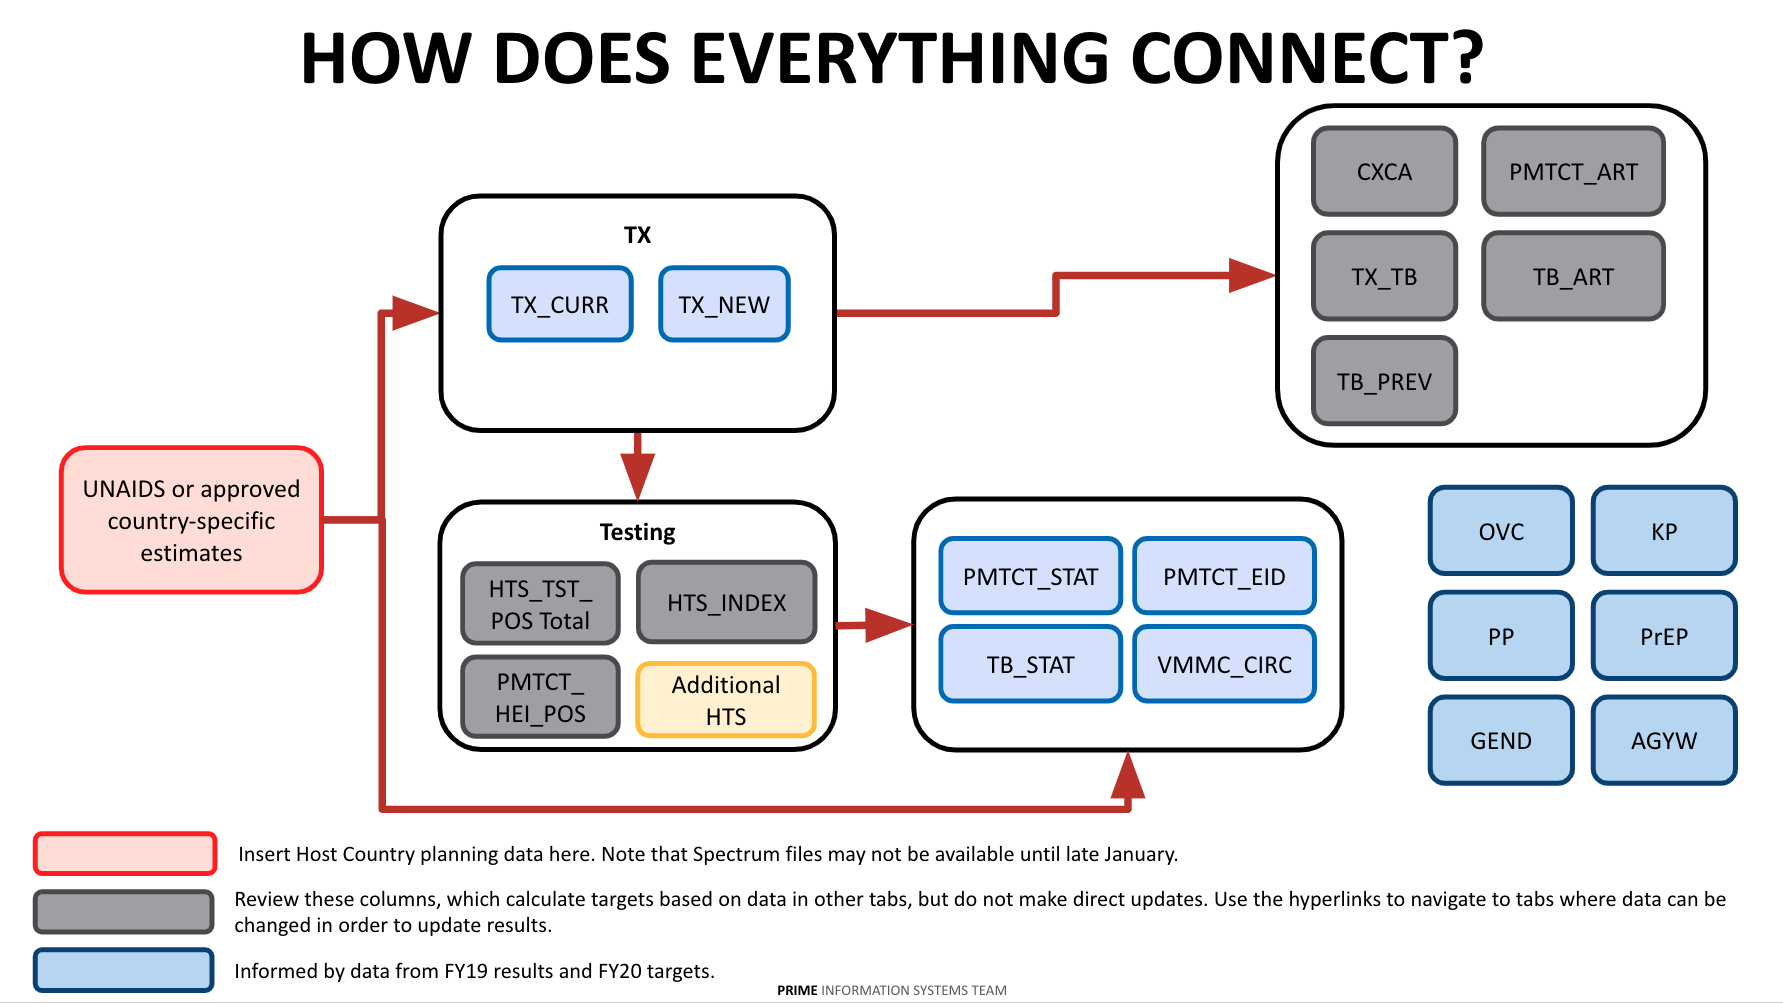
\includegraphics[width=9in]{./images/image3.png}

\end{center}

\newpage

\hypertarget{elements-of-a-tab}{%
\section{Elements of a Tab}\label{elements-of-a-tab}}

\begin{center}

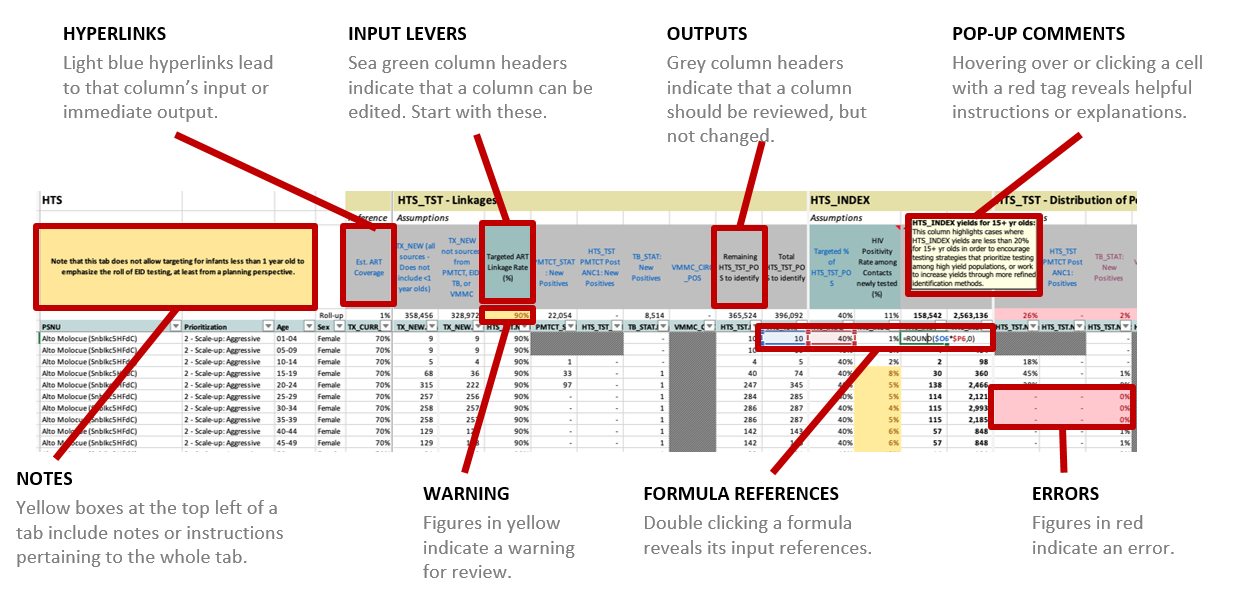
\includegraphics[width=9in]{./images/image4.png}

\end{center}

\newpage

\hypertarget{how-to-navigate-a-data-pack-tab}{%
\section{How to Navigate a Data Pack Tab}\label{how-to-navigate-a-data-pack-tab}}

\begin{center}

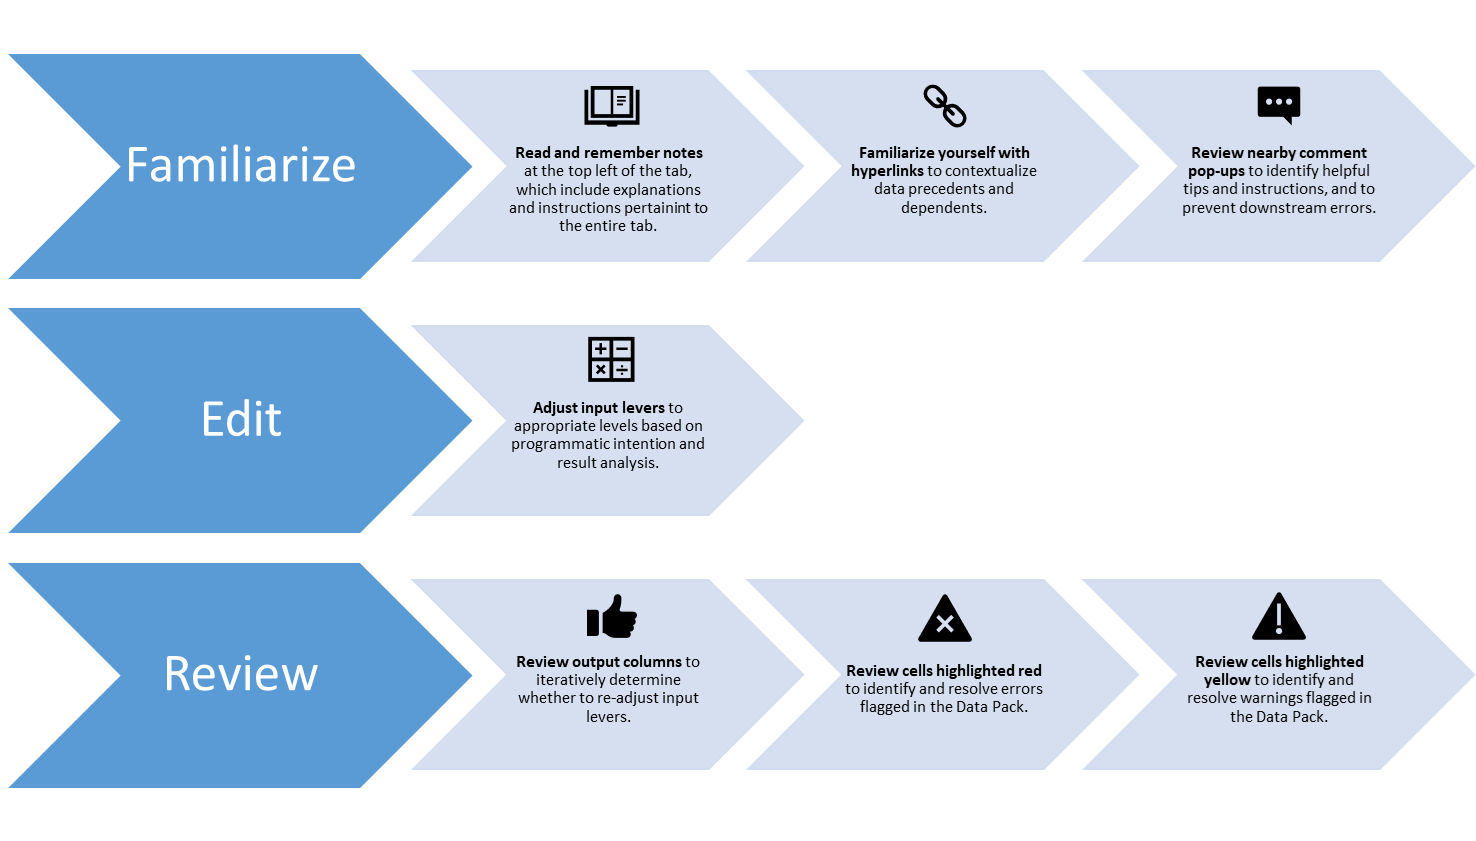
\includegraphics[width=9in]{./images/image5.png}

\end{center}

\elandscape

\newpage

\textbf{ENTERING DATA IN THE CORRECT SECTION}

In the tabs for the DATIM Data Elements, sections may either have data
prepopulated from DATIM or the user will enter data into that column.
Each section of the guide will list what columns users can expect to
have data prepopulated and / or where they can enter data themselves.

\textbf{ENTERING DATA IN THE WRONG SECTION}

If you enter data into a cell that you are not supposed to enter data
into, you will receive the following message box with corrective action
suggestions as well.

\textbf{Example:}

\begin{center}

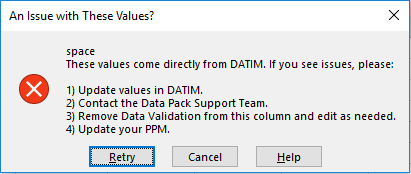
\includegraphics[width=4.3in]{./images/image9.png}

\end{center}

\hypertarget{adjustments-to-historic-targets-and-results}{%
\section{Adjustments to Historic Targets and Results}\label{adjustments-to-historic-targets-and-results}}

Throughout the Data Pack, historic targets and results have been
provided for reference and often to drive target modeling algorithms.
If, in the process of reviewing these historic data, issues with the
data are discovered that may need to be addressed in DATIM, follow the
below procedure:

\begin{enumerate}
\def\labelenumi{\arabic{enumi}.}
\item
  Raise specific issues with historic data to your PPM and DUIT
  Liaison. Determine together whether any issue identified requires
  updating values in DATIM.
\item
  If it is the case that DATIM values should be updated, follow the
  usual process for OPU Target changes, requesting all necessary
  approvals to initiate and expedite this process during COP.
\item
  Once changes are processed in DATIM, you can either request a new
  Data Pack with updated data from DATIM, or copy new values into the
  related column of the Data Pack yourself. For either of these
  routes, reach out to the Data Pack Systems Team via Zendesk for
  support.
\item
  It may also be the case that together with your PPM and DUIT Liaison
  you decide that changes to historic values are not necessary in
  DATIM, but still necessary in the Data Pack. This is an
  extraordinary circumstance and must have approval from DUIT Liaisons
  to allow. If approved, you may make changes directly in the related
  column of the Data Pack.
\end{enumerate}

\newpage

\hypertarget{release-notes}{%
\chapter{Release Notes}\label{release-notes}}

Coming soon!

\hypertarget{whats-new}{%
\chapter{What's New?}\label{whats-new}}

\textbf{HTS Tab Formula Error}

In the HTS Tab there is an error within the formula that helps calculate ``TB\_STAT: New Positive (\%)'' in column Z of the HTS\_TST - Distribution of Positive Tests section. This formula is currently referencing ``HTS\_TST Post ANC1 New Positives (FY22)'' from column J, but needs to be referencing ``TB\_STAT New Positives (FY22)'' from column K. To make this simple change, please adjust the formula from

\[=IF(OR(SUM(\$G15)=0,SUM(\$J15)=0),"",SUM(\$J15)/SUM(\$G15))\]

and change the reference of column J to column K so that it reads

\[=IF(OR(SUM(\$G15)=0,SUM(\$K15)=0),"",SUM(\$K15)/SUM(\$G15))\]

\textbf{PSNUxIM Tab Formulas}

When you received your newly generated PSNUxIM tab for the first time, you will need to scroll to the ``Target Values'' Section that begins in column CW and copy down the formulas populated in row 15 all the way down to the bottom of your Data Pack. This will be required in order for your Rollup column to properly populate as well as the Deduplication sections.

\hypertarget{frequently-asked-questions}{%
\chapter{Frequently Asked Questions}\label{frequently-asked-questions}}

\textbf{\emph{Q: When working through PSNUxIM KP mechanism allocations and I allocate the KP-specific targets to KP partners, given that the KP disags are a subset of the total population being targeted, do I also need to allocate total pop targets to the KP partner?}}

A: Yes, you should be setting a corresponding Total Pop target against each mechanism you set KeyPop targets against. This is because KeyPop is a subset of Total Pop.

\textbf{\emph{Q: Can you use FY22 Spectrum estimates to work through the Cascade tab?}}

A: No, unless you receive approval from OGAC Leadership you should use FY21 Spectrum Data. Your target setting process for the COP21 Data Pack should be to set FY22 targets based on where you are ending FY21.

\textbf{\emph{Q: Is the coverage rate that is used to calculate ``Targeted Host Country TX\_CURR\_SUBNAT (FY22)'' and ``Targeted Host Country TX\_NET\_NEW\_SUBNAT (FY22)'' too high or being miscalculated?}}

A: No, this is not a formula error. The calculations occurring are focusing on PLHIV for each district that are being treated for HIV/AIDS for each age band, as opposed to those being treated for HIV/AIDS in the district regardless of whether they live in that district. if the PEPFAR results are higher than the PLHIV Spectrum estimate in a particular district, then back-calculating the coverage rate shows a greater than 100\% value for that PSNU-Age-Sex band. This can come from one of two things generally: People are coming from outside the district to seek treatment, leading to a higher PEPFAR TX\_CURR value than PLHIV in the district; or The PLHIV estimate from Spectrum is too low. Either way if you have good programmatic reason for doing so, particularly health seeking behavior of PLHIV, you can aim for a coverage rate even higher than 100\% (e.g., current coverage in capital city is estimated at 105\%, but due to health seeking behavior you want to aim for 120\% to achieve 95\% for across all metropolitan area).

\textbf{\emph{Q: Why in the newly generated PSNUxIM tab are data-pack totals and roll up columns blank?}}

A: Once you have regenerated your PSNUxIM tab from the Data Pack Self-Service app, please open your newly regenerated tool, save your tool and close it. When you reopen your tool, it should populate your targets into that column. You will also need to drag down the formula in the far right ``Target Values'' section of the PSNUxIM tab to ensure all rows are populated with the proper formula.

\textbf{\emph{Q: If my program performs testing but not treatment, how do I represent this in the Data Pack?}}

A: You will first need approval from OGAC Leadership to do this. If you receive this approval you will need to manually alter in the Cascade Tab column ``HTS\_TST\_POS + PMTCT\_HEI\_POS (FY22)'' (BD). Please make the alterations to this column and not on the HTS tab.

\textbf{\emph{Q: When I try to validate my Data Pack in the self-service app, I get a message saying ``ERROR: An error has occurred. Check your logs or contact the app author for clarification.'' How do I resolve this?}}

A: This error can be caused by a number of different issues. The most common causes and their resolutions include:

\begin{itemize}
\tightlist
\item
  Trying to validate a newly regenerated Data Pack before opening it and saving it. After generating or regenerating your PSNUxIM tab, it is necessary to first open your tool and save it before uploading it to the app.
\item
  The browser is causing issues with the app. This can be resolved by opening an Incognito window or by clearing your cache. PLEASE NOTE: Clearing your cache will sign you out of all accounts in that browser.
\item
  Trying to validate a file that isn't an XLSX. If your team has saved your Data Pack in a different file format for sharing, such as XLSB, ensure that you resave the file as an XLSX before validating it in the app.
\item
  The target distribution formulas on the PSNUxIM tab have not been applied to all rows. By default, the formulas in the ``Target Value'' section (Column CW and right) are only applied to Row 15. Once you generate or regenerate your PSNUxIM tab, ensure that you copy these formulas all the way down to the bottom row of your targets. After this is done, try validating your tool again.
\end{itemize}

If none of the above issues apply to your Data Pack tool and you are still receiving this error, please submit a ZenDesk ticket identifying your country and attaching or linking to a copy of the Data Pack tool that caused the error in the app.

\hypertarget{how-to-use-the-user-manual}{%
\chapter{How to Use the User Manual}\label{how-to-use-the-user-manual}}

The Data Pack consists of tabs that address indicators related to each
PEPFAR program area.

The COP21 Data Pack User Manual reviews all indicators within each tab
and provides you with the relevant information to complete all required
sections of the Data Pack correctly. It also instructs you where to find
more information on each program area in the COP21 Guidance.

\hypertarget{key-column-highlights}{%
\section{Key Column Highlights}\label{key-column-highlights}}

\begin{quote}
\textbf{\emph{Column type?}} Indicates whether the data in this column is a
result from a previous fiscal year (``Result''), an assumption that the
country team is making (``Assumption''), a target for FY2022
(``Targets''), or a reference for the country team as they fill out the
Data Pack (``Reference'').

\textbf{\emph{What type of data?}} Indicates whether the data in the column is
an integer, e.g.~a whole number, or a percentage.

\textbf{\emph{Prepopulated data?}} Indicates whether the data in this column is
prepopulated from data in DATIM or from data elsewhere in the Data
Pack.

\textbf{\emph{Enter or modify data?}} Indicates whether the user should enter
new information into this column or is allowed to modify the
prepopulated information in the column. If there is a question mark
here, country teams must consult with their PPMs and Chairs before
modifying the data in this column. If there is an exclamation mark
here, country teams may overwrite the formula in this column, however
it will prevent the Data Pack from refreshing this data if changes are
made elsewhere.

\textbf{\emph{Calculated column?}} This indicates that a formula is used to
indicate where a formula is used to calculate the values in this
column from data elsewhere in the Data Pack.

\textbf{\emph{Linked column?}} This indicates that this data is either
prepopulated by or is used to prepopulate data in a column on another
tab within the Data Pack. For columns that are prepopulated from
another tab, clicking on the column name in the Data Pack will take
you to the referenced column.

\emph{\textbf{UID in Appendix}.} The UID provided here is a Data Pack reference
ID and can be used to find more information about the data entered
into this column in the appendices.
\end{quote}

\newpage

\blandscape

\hypertarget{how-to-fill-out-the-data-pack}{%
\chapter{How to Fill Out the Data Pack}\label{how-to-fill-out-the-data-pack}}

\begin{center}

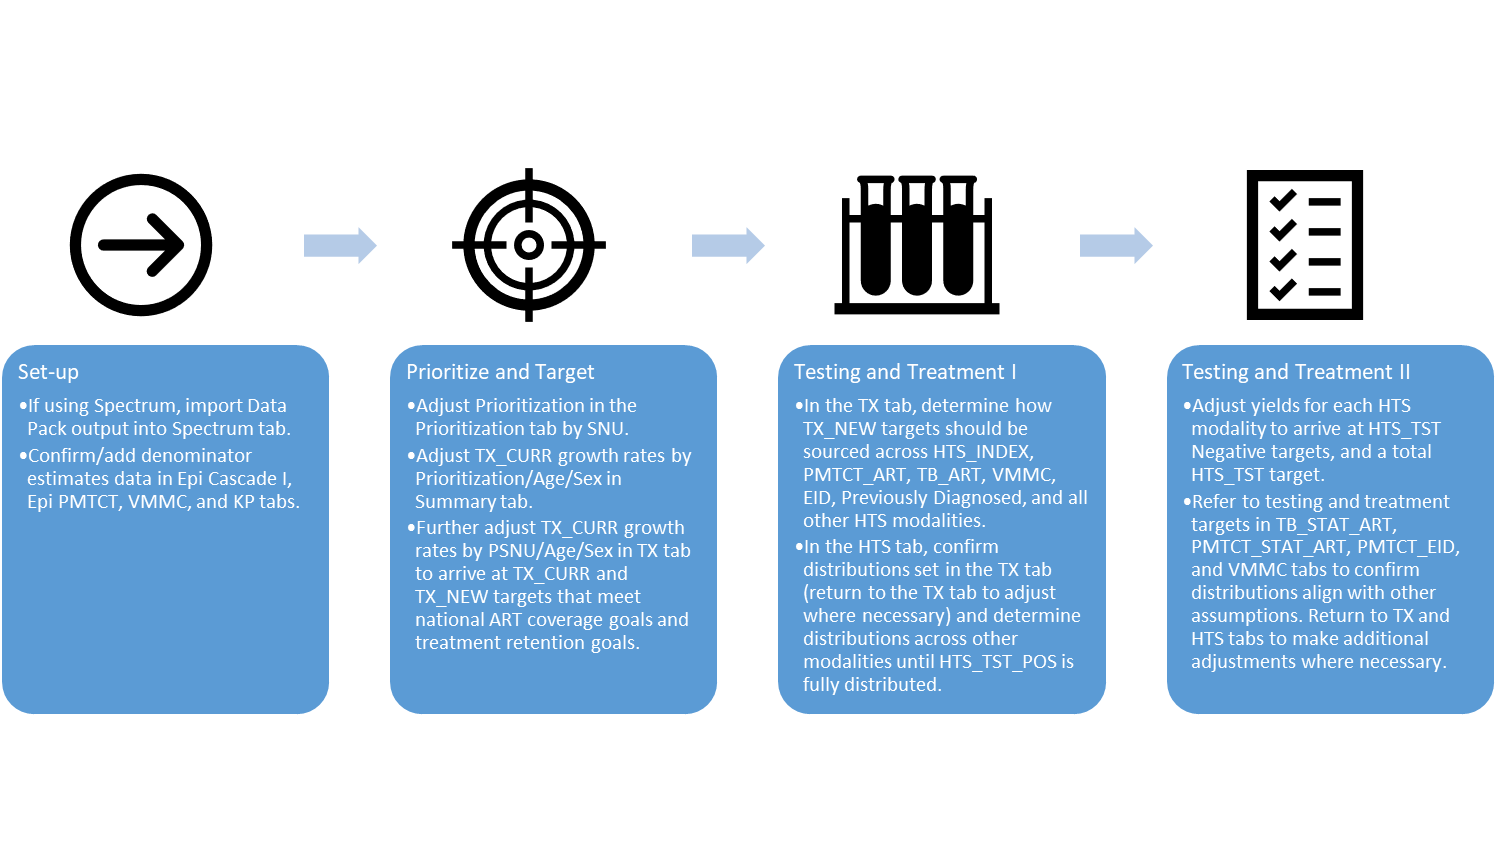
\includegraphics[width=9in]{./images/image12.png}

\end{center}

\newpage

\begin{center}

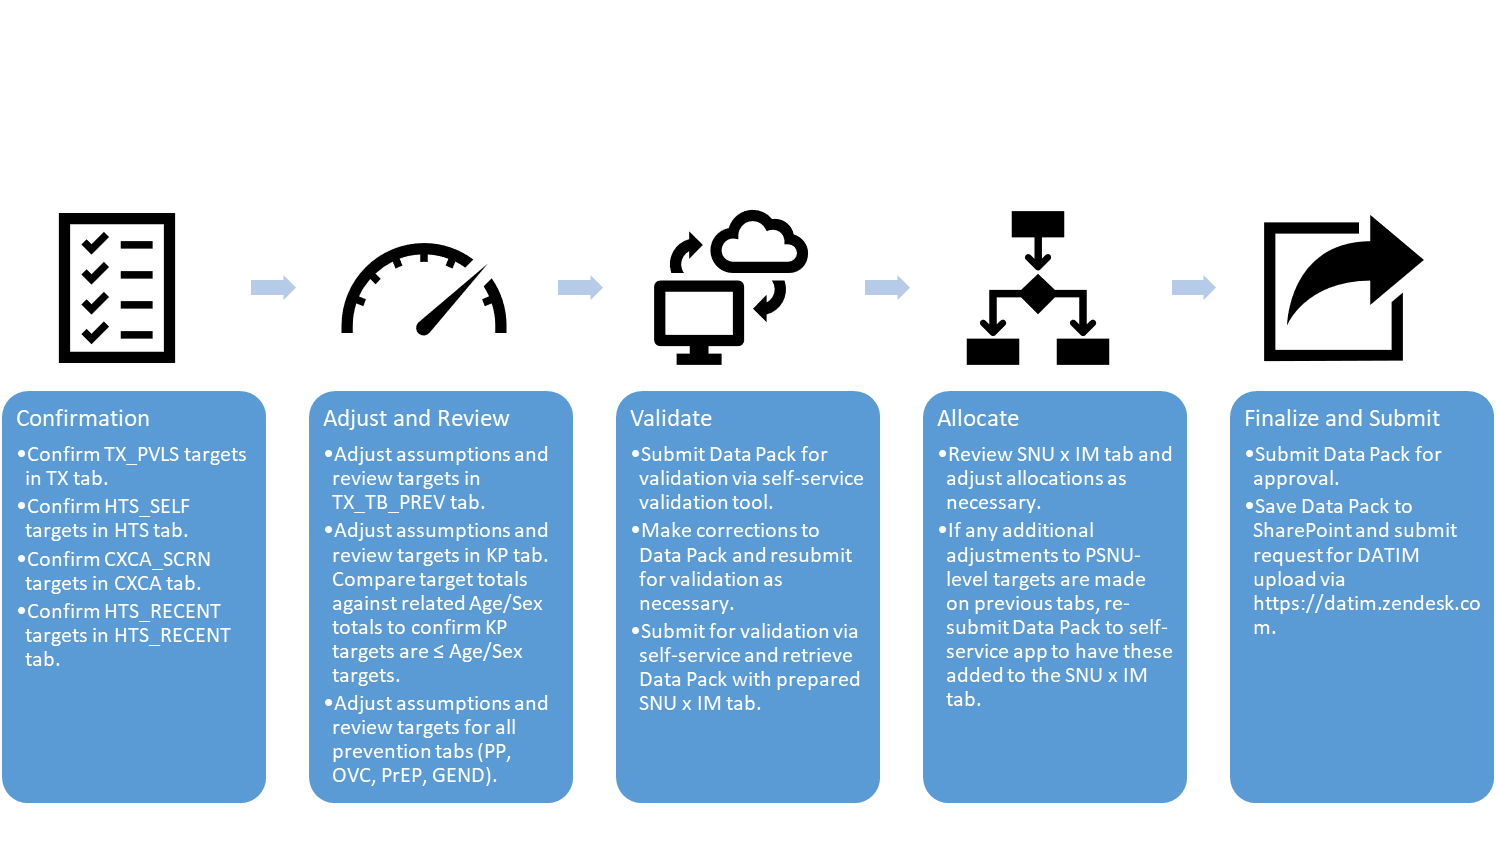
\includegraphics[width=9in]{./images/image13.png}

\end{center}

\elandscape

\newpage

\blandscape

\hypertarget{summary}{%
\chapter{SUMMARY}\label{summary}}

This tab consists of 2 main sections that are listed on the left side
navigation:

\begin{center}

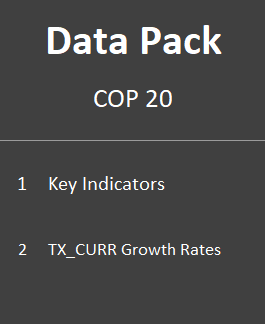
\includegraphics[width=2.2085247156605425in, height=2.7002340332458443in]{./images/image14.png}

\end{center}

Click on either choice to reach the following sections:

\begin{enumerate}
\def\labelenumi{\arabic{enumi}.}
\tightlist
\item
  Key Indicators
\end{enumerate}

\begin{itemize}
\item
  Current ART Coverage
\item
  National Total on ART
\item
  Expected PEPFAR\_TX\_CURR
\item
  Est. Current HIV Prevalence Rate
\end{itemize}

\begin{enumerate}
\def\labelenumi{\arabic{enumi}.}
\setcounter{enumi}{1}
\tightlist
\item
  Targeted PEPFAR TX\_CURR Rates of Change (FY20 to FY21)
\end{enumerate}

\begin{itemize}
\item
  Teams can use this panel to set initial broad FY20-21 growth rates
  for PEPFAR TX\_CURR. Adjust default values to reflect program
  intention. This growth rate table is optional for SNUs who want to
  make broad increases across prioritization level.
\item
  Whether users make changes, all uses should navigate to the TX tab
  to refine growth rates by age/sex and PSNU.
\item
  Changes are made in TX tab will overwrite any changes in this panel.
  After changes are made in the TX tab, the panel will NO LONGER
  affect the final targeted growth rates on the TX tab.
\end{itemize}

\elandscape

\newpage

\blandscape

\hypertarget{spectrum}{%
\chapter{SPECTRUM}\label{spectrum}}

The Spectrum tab will allow users to load UNAIDS data with 12 columns of
data elements for your OU. A Spectrum file for your OU will be provided
at the conclusion of the UNAIDS Spectrum Training for Country Teams. The
contents of this file will be manually loaded into the Spectrum tab
which is setup as below:

\begin{table}[H]
\centering\begingroup\fontsize{12}{14}\selectfont

\resizebox{\linewidth}{!}{
\begin{tabular}{l>{\raggedright\arraybackslash}p{1.25in}>{\raggedright\arraybackslash}p{1.25in}>{\raggedright\arraybackslash}p{1.25in}>{\raggedright\arraybackslash}p{1.25in}>{\raggedright\arraybackslash}p{1.25in}>{\raggedright\arraybackslash}p{1.25in}}
\toprule
\multicolumn{1}{c}{\cellcolor[HTML]{E6DFA7}{ }} & \multicolumn{1}{>{\centering\arraybackslash}p{1.25in}}{\cellcolor[HTML]{E6DFA7}{D}} & \multicolumn{1}{>{\centering\arraybackslash}p{1.25in}}{\cellcolor[HTML]{E6DFA7}{E}} & \multicolumn{1}{>{\centering\arraybackslash}p{1.25in}}{\cellcolor[HTML]{E6DFA7}{F}} & \multicolumn{1}{>{\centering\arraybackslash}p{1.25in}}{\cellcolor[HTML]{E6DFA7}{G}} & \multicolumn{1}{>{\centering\arraybackslash}p{1.25in}}{\cellcolor[HTML]{E6DFA7}{H}} & \multicolumn{1}{>{\centering\arraybackslash}p{1.25in}}{\cellcolor[HTML]{E6DFA7}{I}}\\
\midrule
Column Name & psnu & psnu\_uid & area\_id & indicator\_code & dataelement\_uid & age\\
Column Type? & NA & NA & NA & NA & NA & NA\\
What type of data? & string & string & string & string & string & string\\
Prepopulated data? & N & N & N & N & N & N\\
Enter or modify data? & Y & Y & Y & Y & Y & Y\\
\addlinespace
Calculated column? & N & N & N & N & N & N\\
Linked column? & N & N & N & N & N & N\\
\bottomrule
\end{tabular}}
\endgroup{}
\end{table}

\begin{table}[H]
\centering\begingroup\fontsize{12}{14}\selectfont

\resizebox{\linewidth}{!}{
\begin{tabular}{l>{\raggedright\arraybackslash}p{1.25in}>{\raggedright\arraybackslash}p{1.25in}>{\raggedright\arraybackslash}p{1.25in}>{\raggedright\arraybackslash}p{1.25in}>{\raggedright\arraybackslash}p{1.25in}>{\raggedright\arraybackslash}p{1.25in}}
\toprule
\multicolumn{1}{c}{\cellcolor[HTML]{E6DFA7}{ }} & \multicolumn{1}{>{\centering\arraybackslash}p{1.25in}}{\cellcolor[HTML]{E6DFA7}{J}} & \multicolumn{1}{>{\centering\arraybackslash}p{1.25in}}{\cellcolor[HTML]{E6DFA7}{K}} & \multicolumn{1}{>{\centering\arraybackslash}p{1.25in}}{\cellcolor[HTML]{E6DFA7}{L}} & \multicolumn{1}{>{\centering\arraybackslash}p{1.25in}}{\cellcolor[HTML]{E6DFA7}{M}} & \multicolumn{1}{>{\centering\arraybackslash}p{1.25in}}{\cellcolor[HTML]{E6DFA7}{N}} & \multicolumn{1}{>{\centering\arraybackslash}p{1.25in}}{\cellcolor[HTML]{E6DFA7}{O}}\\
\midrule
Column Name & age\_uid & sex & sex\_uid & calendar\_quarter & value & age\_sex\_rse\\
Column Type? & NA & NA & NA & NA & NA & NA\\
What type of data? & string & string & string & string & string & string\\
Prepopulated data? & N & N & N & N & N & N\\
Enter or modify data? & Y & Y & Y & Y & Y & Y\\
\addlinespace
Calculated column? & N & N & N & N & N & N\\
Linked column? & N & N & N & N & N & N\\
\bottomrule
\end{tabular}}
\endgroup{}
\end{table}

With S/GAC approval, countries can also populate input their own data
into this tab with a different MOH/ country approved set of estimates.
Estimate changes can also be made in the two associated tabs, Cascade
and PMTCT.

\elandscape

\newpage

\blandscape

\hypertarget{prioritization}{%
\chapter{PRIORITIZATION}\label{prioritization}}

\begin{table}[H]
\centering\begingroup\fontsize{12}{14}\selectfont

\resizebox{\linewidth}{!}{
\begin{tabular}{l>{\raggedright\arraybackslash}p{2.5in}>{\raggedright\arraybackslash}p{2.5in}>{\raggedright\arraybackslash}p{2.5in}}
\toprule
\multicolumn{1}{c}{\cellcolor[HTML]{E6DFA7}{ }} & \multicolumn{1}{>{\centering\arraybackslash}p{2.5in}}{\cellcolor[HTML]{E6DFA7}{B}} & \multicolumn{1}{>{\centering\arraybackslash}p{2.5in}}{\cellcolor[HTML]{E6DFA7}{C}} & \multicolumn{1}{>{\centering\arraybackslash}p{2.5in}}{\cellcolor[HTML]{E6DFA7}{D}}\\
\midrule
Column Name & NA & SNU Prioritization (FY21) & SNU Prioritization (FY22)\\
UID & PSNU & IMPATT.PRIORITY\_SNU.T\_1 & IMPATT.PRIORITY\_SNU.T\\
Column Type? & row\_header & past & target\\
What type of data? & string & integer & integer\\
Prepopulated data? & N & Y & N\\
\addlinespace
Enter or modify data? & N & ? & N\\
Calculated column? & Y & N & Y\\
Linked column? & N & N & N\\
\bottomrule
\end{tabular}}
\endgroup{}
\end{table}

\hypertarget{datim-import}{%
\subsection{DATIM Import}\label{datim-import}}

The following data points will be imported into DATIM from this section:

\begin{itemize}
\tightlist
\item
  \textbf{SNU Prioritization (FY22)} {[}IMPATT.PRIORITY\_SNU.T{]}
\end{itemize}

\hypertarget{instructions}{%
\subsection{Instructions}\label{instructions}}

\begin{enumerate}
\def\labelenumi{\arabic{enumi}.}
\item
  Review the column ``SNU Prioritization (FY21)'' which will indicate
  prioritization levels set in COP20 for each PSNU.
\item
  Review ``SNU Prioritization (FY22)'' and adjust as appropriate for
  COP21 programming. This is currently set to populate with the same
  level of prioritization that was referenced in step 1. Overwrite
  this column to set new levels of prioritization based on the list
  below. This column should only be populated using integers 1-8 and
  ``M'', ``NA'', or ``Not a PSNU'', as follows:

  \begin{enumerate}
  \def\labelenumii{\alph{enumii}.}
  \item
    1 = "Scale-up: Saturation"
  \item
    2 = "Scale-up: Aggressive"
  \item
    4 = "Sustained"
  \item
    5 = "Centrally Supported"
  \item
    6 = ``Sustained: Commodities''
  \item
    7 = "Attained"
  \item
    8 = "Not PEPFAR Supported"
  \item
    ``M'' = "Military"
  \item
    "NA","Not a PSNU" = "INVALID"
  \end{enumerate}
\item
  Review the column ``FY22 SNU Prioritization Translation'' to ensure
  the prioritization level for each PSNU is correct. To make any
  changes, only edit the column ``SNU Prioritization (FY22)'' from
  Step 2.
\end{enumerate}

\elandscape

\newpage

\blandscape

\hypertarget{cascade}{%
\chapter{CASCADE}\label{cascade}}

The Cascade Tab allows Data Pack users to view and set the overall
contour of their treatment and testing program across both geography and
population. This tab, new to the COP21 Data Pack, is a consolidation of
some elements of the TX and HTS tabs present in previous Data Pack
versions, and begins with an analysis of gap to ART coverage
disaggregated by geography and population, then uses this analysis to
progress through modeling of first treatment, then viral load
suppression, and finally testing targets.

This tab also links heavily with many other tabs of the Data Pack,
including the PMTCT, TB, EID, VMMC, HTS, CXCA, HTS\_RECENT, TX\_TB\_PREV,
and KP tabs. By beginning with the Cascade tab, moving through each of
these other tabs, and continually returning to the Cascade tab to
monitor and iteratively adjust the overall program plan, Country Teams
can both retain a cohesive and intentional strategy across program area,
geography, and population, as well as anchor this strategy in data and
the realities of past performance.

\hypertarget{host-country-context}{%
\section{Host Country Context}\label{host-country-context}}

\begin{table}[H]
\centering\begingroup\fontsize{12}{14}\selectfont

\resizebox{\linewidth}{!}{
\begin{tabular}{l>{\raggedright\arraybackslash}p{1.875in}>{\raggedright\arraybackslash}p{1.875in}>{\raggedright\arraybackslash}p{1.875in}>{\raggedright\arraybackslash}p{1.875in}}
\toprule
\multicolumn{1}{c}{\cellcolor[HTML]{E6DFA7}{ }} & \multicolumn{1}{>{\centering\arraybackslash}p{1.875in}}{\cellcolor[HTML]{E6DFA7}{F}} & \multicolumn{1}{>{\centering\arraybackslash}p{1.875in}}{\cellcolor[HTML]{E6DFA7}{G}} & \multicolumn{1}{>{\centering\arraybackslash}p{1.875in}}{\cellcolor[HTML]{E6DFA7}{H}} & \multicolumn{1}{>{\centering\arraybackslash}p{1.875in}}{\cellcolor[HTML]{E6DFA7}{I}}\\
\midrule
Column Name & Host Country Est. Population (FY21) & RSE: Population (District-level) & Host Country Est. PLHIV (FY21) & RSE: PLHIV (District-level)\\
UID & POP\_EST.T\_1 & POP\_EST.DistrictUncertainty & PLHIV.T\_1 & PLHIV.DistrictUncertainty\\
Column Type? & target & reference & target & reference\\
What type of data? & integer & percentage & integer & percentage\\
Prepopulated data? & N & N & N & N\\
\addlinespace
Enter or modify data? & N & N & N & N\\
Calculated column? & Y & Y & Y & Y\\
Linked column? & N & N & N & N\\
\bottomrule
\end{tabular}}
\endgroup{}
\end{table}

\begin{table}[H]
\centering\begingroup\fontsize{12}{14}\selectfont

\resizebox{\linewidth}{!}{
\begin{tabular}{l>{\raggedright\arraybackslash}p{1.875in}>{\raggedright\arraybackslash}p{1.875in}>{\raggedright\arraybackslash}p{1.875in}>{\raggedright\arraybackslash}p{1.875in}}
\toprule
\multicolumn{1}{c}{\cellcolor[HTML]{E6DFA7}{ }} & \multicolumn{1}{>{\centering\arraybackslash}p{1.875in}}{\cellcolor[HTML]{E6DFA7}{J}} & \multicolumn{1}{>{\centering\arraybackslash}p{1.875in}}{\cellcolor[HTML]{E6DFA7}{K}} & \multicolumn{1}{>{\centering\arraybackslash}p{1.875in}}{\cellcolor[HTML]{E6DFA7}{L}} & \multicolumn{1}{>{\centering\arraybackslash}p{1.875in}}{\cellcolor[HTML]{E6DFA7}{M}}\\
\midrule
Column Name & Host Country Est. HIV Prevalence (FY21) (\%) & RSE: HIV Prevalence (District-level) & Host Country Est. PLHIV who know HIV Status (FY21) & Host Country Est. \% PLHIV who know HIV Status (FY21) (\%)\\
UID & HIV\_PREV.T\_1 & HIV\_PREV.DistrictUncertainty & DIAGNOSED\_SUBNAT.T\_1 & DIAGNOSED\_SUBNAT.Rt.T\_1\\
Column Type? & target & reference & target & reference\\
What type of data? & percentage & percentage & integer & percentage\\
Prepopulated data? & N & N & N & N\\
\addlinespace
Enter or modify data? & N & N & N & N\\
Calculated column? & Y & Y & Y & Y\\
Linked column? & N & N & N & N\\
\bottomrule
\end{tabular}}
\endgroup{}
\end{table}

\begin{table}[H]
\centering\begingroup\fontsize{12}{14}\selectfont

\resizebox{\linewidth}{!}{
\begin{tabular}{l>{\raggedright\arraybackslash}p{2.5in}>{\raggedright\arraybackslash}p{2.5in}>{\raggedright\arraybackslash}p{2.5in}}
\toprule
\multicolumn{1}{c}{\cellcolor[HTML]{E6DFA7}{ }} & \multicolumn{1}{>{\centering\arraybackslash}p{2.5in}}{\cellcolor[HTML]{E6DFA7}{N}} & \multicolumn{1}{>{\centering\arraybackslash}p{2.5in}}{\cellcolor[HTML]{E6DFA7}{O}} & \multicolumn{1}{>{\centering\arraybackslash}p{2.5in}}{\cellcolor[HTML]{E6DFA7}{P}}\\
\midrule
Column Name & Host Country Observed TX\_CURR\_SUBNAT (FY20) & RSE: TX\_CURR\_SUBNAT.R (District-level) & Host Country Est. TX\_CURR\_SUBNAT (FY21)\\
UID & TX\_CURR\_SUBNAT.R & TX\_CURR\_SUBNAT.DistrictUncertainty.R & TX\_CURR\_SUBNAT.T\_1\\
Column Type? & target & reference & target\\
What type of data? & integer & percentage & integer\\
Prepopulated data? & N & N & N\\
\addlinespace
Enter or modify data? & N & N & N\\
Calculated column? & Y & Y & Y\\
Linked column? & N & N & N\\
\bottomrule
\end{tabular}}
\endgroup{}
\end{table}

\begin{table}[H]
\centering\begingroup\fontsize{12}{14}\selectfont

\resizebox{\linewidth}{!}{
\begin{tabular}{l>{\raggedright\arraybackslash}p{2.5in}>{\raggedright\arraybackslash}p{2.5in}>{\raggedright\arraybackslash}p{2.5in}}
\toprule
\multicolumn{1}{c}{\cellcolor[HTML]{E6DFA7}{ }} & \multicolumn{1}{>{\centering\arraybackslash}p{2.5in}}{\cellcolor[HTML]{E6DFA7}{Q}} & \multicolumn{1}{>{\centering\arraybackslash}p{2.5in}}{\cellcolor[HTML]{E6DFA7}{R}} & \multicolumn{1}{>{\centering\arraybackslash}p{2.5in}}{\cellcolor[HTML]{E6DFA7}{S}}\\
\midrule
Column Name & RSE: TX\_CURR\_SUBNAT.T\_1 (District-level) & Host Country Est. Virally Suppressed ART Patients (FY21) & Host Country Est. Viral Load Suppression Rate (FY21) (\%)\\
UID & TX\_CURR\_SUBNAT.DistrictUncertainty.T\_1 & VL\_SUPPRESSED.T\_1 & VL\_SUPPRESSED.Rt.T\_1\\
Column Type? & reference & target & reference\\
What type of data? & percentage & integer & percentage\\
Prepopulated data? & N & N & N\\
\addlinespace
Enter or modify data? & N & N & N\\
Calculated column? & Y & Y & Y\\
Linked column? & N & N & N\\
\bottomrule
\end{tabular}}
\endgroup{}
\end{table}

For those leveraging UNAIDS Spectrum estimate exports for the Data Pack,
once these have been loaded into the Spectrum tab of the Data Pack, this
first portion of the Cascade tab will automatically update to reflect
these estimates.

In specific, the Host Country Context section of the Cascade tab
provides space for reflecting estimates from either Spectrum or an
alternative approved source for the following data:

\begin{itemize}
\item
  Host Country Estimated Population (FY21) {[}POP\_EST.T\_1{]}: Estimated
  population, projected as of September 2021.
\item
  \textbf{Host Country Estimated PLHIV (FY21) {[}PLHIV.T\_1{]}:} Estimated
  number of people living with HIV, projected as of September 2021.
\item
  Host Country Estimated HIV Prevalence (FY21) {[}HIV\_PREV.T\_1{]}:
  Estimated HIV Prevalence, projected as of September 2021.
\item
  Host Country Estimated PLHIV who Know HIV Status (FY21)
  {[}DIAGNOSED\_SUBNAT.T\_1{]}: Estimated PLHIV who know their HIV status,
  projected as of September 2021.
\item
  \textbf{Host Country Observed TX\_CURR\_SUBNAT (FY20)
  {[}TX\_CURR\_SUBNAT.R{]}:} Observed/actual total number of PLHIV
  receiving ART as of September 2020.
\item
  \textbf{Host Country Estimated TX\_CURR\_SUBNAT (FY21)
  {[}TX\_CURR\_SUBNAT.T\_1{]}:} Estimated number of PLHIV receiving ART,
  projected as of September 2021.
\item
  Host Country Estimated Virally Suppressed ART Patients
  {[}VL\_SUPPRESSION\_SUBNAT.T\_1{]}: Estimated PLHIV on ART and virally
  suppressed, projected as of September 2021.
\end{itemize}

\hypertarget{datim-import-1}{%
\subsection{DATIM Import}\label{datim-import-1}}

As part of the Data Pack approval process, all of the above FY21
projected estimates will be uploaded into DATIM and replace any
preexisting estimates for these indicators that may have already been
entered in DATIM, perhaps via Data Pack upload during COP20.

\hypertarget{instructions-1}{%
\subsection{Instructions}\label{instructions-1}}

\begin{enumerate}
\def\labelenumi{\arabic{enumi}.}
\item
  If using UNAIDS Spectrum as the source for these data:

  \begin{enumerate}
  \def\labelenumii{\alph{enumii}.}
  \item
    Review the above columns to confirm that data has been correctly
    linked with the Spectrum tab. You may consider using filter
    drop-down menus to quickly inspect for any non-numeric,
    negative, or invalid data.
  \item
    Review Relative Standard Error values to identify any estimates
    with a Relative Standard Error of more than or equal to 20. See
    the section below for additional instructions.
  \end{enumerate}
\item
  If not using UNAIDS Spectrum as the source for these data, see the
  below section.
\item
  Confirm that no data has been entered against Military Organization
  Units. See below for more explanation.
\end{enumerate}

\hypertarget{leveraging-alternatives-to-spectrum}{%
\subsection{Leveraging Alternatives to Spectrum}\label{leveraging-alternatives-to-spectrum}}

In general, all data for the above should use UNAIDS Spectrum as their
source. However, there may be cases where either a more up to date or
reliable source exists, or where data may not be fully available from
UNAIDS Spectrum. In these cases, Country Teams may request approval from
their PPM and a DUIT Liaison to use an alternative data source. Be sure
to request and document this approval before deciding not to use
Spectrum as the source for your Data Pack host country estimates, as
well as what source is approved for use in its place. This is true for
all cases where you may need to leverage an alternative to Spectrum,
whether for an entire indicator, or for a specific geography or
population.

For those not leveraging Spectrum to provide host country context
estimates, you may paste estimates from other approved sources into this
section of the Cascade tab by overwriting the formulas currently in
these columns. Due to hidden Relative Standard Error columns between the
various estimate columns, it is recommended you paste this data in one
column at a time, rather than in bulk. It may also reduce technical
issues to first copy geographic data in the SNU1, PSNU, Age, and Sex
columns into a separate spreadsheet, then use Excel lookup functions to
add estimates data against the correct geographies and populations, and
then return to pasting data into the original Cascade tab column by
column.

\hypertarget{relative-standard-errors}{%
\subsection{Relative Standard Errors}\label{relative-standard-errors}}

Data exported from UNAIDS Spectrum will also come with a series Relative
Standard Errors for each data point, both at the District level as well
as the Age/Sex-specific level. Along with the data points listed above,
Relative Standard Errors for each will also automatically be populated
in the Cascade tab from data loaded into the Spectrum tab. While
initially, these Error columns will be hidden, you may inspect these
values by unhiding these columns. Based on these Relative Standard
Errors, data points in related columns will be color-coded to indicate
the relative uncertainty of each specific data point along the following
ranges:

\begin{itemize}
\item
  Red: Relative Standard Error of 40 or greater.
\item
  Yellow: Relative Standard Error of less than 40, but more than or
  equal to 20.
\item
  Green: Relative Standard Error of less than 20.
\end{itemize}

While these error estimates are available as a reference as teams
formulate targets, red or yellow highlighting may not always mean a data
point should be thrown out, nor is it the case that all green values
should be taken at face value. Either way, consider these error
estimates as helpful guideposts in interpreting the contextual meaning
and data quality of data provided via UNAIDS Spectrum output.

If, in reviewing Relative Standard Error values, the uncertainty
interval of an estimate appears to be concerning, consider the following
next steps:

\begin{enumerate}
\def\labelenumi{\arabic{enumi}.}
\item
  Raise and discuss the issue with your PPM and DUIT Liaison.
\item
  Communicate concerns to assigned UNAIDS liaisons and discuss
  appropriate methods for improving or better understanding data
  quality for the data points in question.
\end{enumerate}

\hypertarget{host-country-estimates-for-military-organization-units}{%
\subsection{Host Country Estimates for Military Organization Units}\label{host-country-estimates-for-military-organization-units}}

Due to issues of political sensitivity and national security, estimates
for the above indicators should not be entered against Military
Organization Units. Any case where this does occur will be flagged in
the Data Pack Self-Service App, and removed during DATIM import.

\hypertarget{cascade-tx_net_new_subat}{%
\section{Cascade: TX\_NET\_NEW\_SUBAT}\label{cascade-tx_net_new_subat}}

\begin{table}[H]
\centering\begingroup\fontsize{12}{14}\selectfont

\resizebox{\linewidth}{!}{
\begin{tabular}{l>{\raggedright\arraybackslash}p{2.5in}>{\raggedright\arraybackslash}p{2.5in}>{\raggedright\arraybackslash}p{2.5in}}
\toprule
\multicolumn{1}{c}{\cellcolor[HTML]{E6DFA7}{ }} & \multicolumn{1}{>{\centering\arraybackslash}p{2.5in}}{\cellcolor[HTML]{E6DFA7}{T}} & \multicolumn{1}{>{\centering\arraybackslash}p{2.5in}}{\cellcolor[HTML]{E6DFA7}{U}} & \multicolumn{1}{>{\centering\arraybackslash}p{2.5in}}{\cellcolor[HTML]{E6DFA7}{V}}\\
\midrule
Column Name & PEPFAR TX\_CURR (FY20 Results) & PEPFAR TX\_CURR (FY21 Targets) & PEPFAR TX\_NET\_NEW (FY21 Targets)\\
UID & TX\_CURR.R & TX\_CURR.T\_1 & TX\_NET\_NEW.T\_1\\
Column Type? & past & past & reference\\
What type of data? & integer & integer & integer\\
Prepopulated data? & Y & Y & N\\
\addlinespace
Enter or modify data? & ? & ? & N\\
Calculated column? & N & N & Y\\
Linked column? & N & N & N\\
\bottomrule
\end{tabular}}
\endgroup{}
\end{table}

\begin{table}[H]
\centering\begingroup\fontsize{12}{14}\selectfont

\resizebox{\linewidth}{!}{
\begin{tabular}{l>{\raggedright\arraybackslash}p{2.5in}>{\raggedright\arraybackslash}p{2.5in}>{\raggedright\arraybackslash}p{2.5in}}
\toprule
\multicolumn{1}{c}{\cellcolor[HTML]{E6DFA7}{ }} & \multicolumn{1}{>{\centering\arraybackslash}p{2.5in}}{\cellcolor[HTML]{E6DFA7}{W}} & \multicolumn{1}{>{\centering\arraybackslash}p{2.5in}}{\cellcolor[HTML]{E6DFA7}{X}} & \multicolumn{1}{>{\centering\arraybackslash}p{2.5in}}{\cellcolor[HTML]{E6DFA7}{Y}}\\
\midrule
Column Name & PEPFAR Coverage of Host Country TX\_CURR\_SUBNAT (FY21) (\%) & PEPFAR Coverage of Host Country TX\_NET\_NEW\_SUBNAT (FY22) (\%) & Host Country Est. ART Coverage (FY21) (\%)\\
UID & TX\_CURR.NatlContr.T\_1 & TX\_CURR.NatlContr.T & TX\_CURR\_SUBNAT.Rt.T\_1\\
Column Type? & reference & assumption & reference\\
What type of data? & percentage & percentage & percentage\\
Prepopulated data? & N & N & N\\
\addlinespace
Enter or modify data? & N & N & N\\
Calculated column? & Y & Y & Y\\
Linked column? & N & N & N\\
\bottomrule
\end{tabular}}
\endgroup{}
\end{table}

\begin{table}[H]
\centering\begingroup\fontsize{12}{14}\selectfont

\resizebox{\linewidth}{!}{
\begin{tabular}{l>{\raggedright\arraybackslash}p{2.5in}>{\raggedright\arraybackslash}p{2.5in}>{\raggedright\arraybackslash}p{2.5in}}
\toprule
\multicolumn{1}{c}{\cellcolor[HTML]{E6DFA7}{ }} & \multicolumn{1}{>{\centering\arraybackslash}p{2.5in}}{\cellcolor[HTML]{E6DFA7}{Z}} & \multicolumn{1}{>{\centering\arraybackslash}p{2.5in}}{\cellcolor[HTML]{E6DFA7}{AA}} & \multicolumn{1}{>{\centering\arraybackslash}p{2.5in}}{\cellcolor[HTML]{E6DFA7}{AB}}\\
\midrule
Column Name & Targeted Host Country ART Coverage (FY22) (\%) & Targeted Host Country TX\_CURR\_SUBNAT (FY22) & Targeted Host Country TX\_NET\_NEW\_SUBNAT (FY22)\\
UID & TX\_CURR\_SUBNAT.Rt.T & TX\_CURR\_SUBNAT.T & TX\_NET\_NEW\_SUBNAT.T\\
Column Type? & assumption & target & reference\\
What type of data? & percentage & integer & integer\\
Prepopulated data? & N & N & N\\
\addlinespace
Enter or modify data? & N & N & N\\
Calculated column? & Y & Y & Y\\
Linked column? & N & N & N\\
\bottomrule
\end{tabular}}
\endgroup{}
\end{table}

This section of the Cascade tab builds upon the preceding Host Country
Context section to arrive at an analysis of gap to ART coverage by
geography and population. This analysis, in concert with projected goals
for ART coverage to be attained by the end of FY22, then helps Data Pack
users simulate the required net new amount of individuals (those added
less those lost to follow-up) to be added to host country ART totals.

\hypertarget{datim-import-2}{%
\subsection{DATIM Import}\label{datim-import-2}}

The following data points will be imported into DATIM from this section:

\begin{itemize}
\tightlist
\item
  \textbf{Targeted Host Country TX\_CURR\_SUBNAT (FY22)} {[}TX\_CURR\_SUBNAT.T{]}
\end{itemize}

\hypertarget{instructions-2}{%
\subsection{Instructions}\label{instructions-2}}

\begin{enumerate}
\def\labelenumi{\arabic{enumi}.}
\item
  Review historic PEPFAR TX\_CURR and TX\_NET\_NEW data to understand
  existing trends and status of TX\_CURR by geography and population.
\item
  Review estimates of PEPFAR Coverage of Host Country
  TX\_NET\_NEW\_SUBNAT and adjust as necessary. See below for additional
  information.
\item
  Review baseline Host Country Estimated ART Coverage.
\item
  Review and adjust Targeted Host Country ART Coverage. See below for
  additional information
\item
  Review resulting \textbf{Targeted Host Country TX\_CURR\_SUBNAT} and
  \textbf{Targeted Host Country TX\_NET\_NEW\_SUBNAT}. See below for
  additional information.
\end{enumerate}

\hypertarget{pepfar-coverage-of-host-country-tx_net_new_subnat}{%
\subsection{PEPFAR Coverage of Host Country TX\_NET\_NEW\_SUBNAT}\label{pepfar-coverage-of-host-country-tx_net_new_subnat}}

In the next section of the Data Pack, the TX\_NET\_NEW\_SUBNAT determined
in this section will be used to estimate necessary PEPFAR TX\_NET\_NEW.

To estimate PEPFAR's contribution to total TX\_NET\_NEW\_SUBNAT in the
country, the Data Pack compares PEPFAR's most recent APR results for
TX\_CURR against the observed host country TX\_CURR\_SUBNAT results ---
sourced from UNAIDS Spectrum, or an alternative approved source, as
described in the Host Country Context section prior to this --- for the
same time period.

While the behavior of PEPFAR and Host Country TX\_CURR may differ from
that of TX\_NET\_NEW, this gives a baseline from which to begin, and
ultimately you may adjust this baseline in the green column titled
``\textbf{PEPFAR Coverage of Host Country TX\_NET\_NEW\_SUBNAT (FY22) (\%)}'' to
more accurately reflect the likely reality of PEPFAR's contribution to
TX\_NET\_NEW\_SUBNAT.

\hypertarget{targeted-host-country-art-coverage}{%
\subsection{Targeted Host Country ART Coverage}\label{targeted-host-country-art-coverage}}

One of the most pivotal data points in the Data Pack is the baseline
estimate of Host Country ART Coverage. To calculate the estimated Host
Country ART Coverage for FY21 (i.e., projected as of September 2021),
the Data Pack uses the following formula:

\begin{center} $\frac{Host\ Country\ Observed\ TX\_ CURR\_ SUBNAT\ (FY20)}{Host\ Country\ Est.\ PLHIV\ (FY21)}$ \end{center}

In the case that PEPFAR's reported TX\_CURR results for FY20 exceed the
reported Host Country Observed TX\_CURR\_SUBNAT for FY20, the following
function will be used to calculate ART Coverage instead of the above:

\begin{center} $\frac{PEPFAR\ TX\_ CURR\ (FY20\ Results)}{Host\ Country\ Est.\ PLHIV\ (FY21)}$ \end{center}

Reviewing and understanding the ART Coverage estimate arrived at in this
column is critical for much of the rest of the Data Pack. In particular,
this column is later instrumental in determining the following key data
points:

\begin{itemize}
\item
  Host Country TX\_CURR\_SUBNAT
\item
  Host Country TX\_NET\_NEW\_SUBNAT
\item
  PEPFAR TX\_CURR
\item
  PEPFAR TX\_NEW
\item
  PEPFAR TX\_PVLS
\item
  PEPFAR HTS\_TST totals
\item
  PEPFAR HTS\_INDEX
\end{itemize}

After reviewing data in this column, examine the next column, \textbf{Targeted
Host Country ART Coverage (FY22) (\%)}. In line with the UNAIDS 95-95-95
goals, this column defaults to 90\%, reflecting that since the
denominator in the Data Pack calculation is Host Country Estimated PLHIV
instead of only those PLHIV who know their HIV Status, this column
should be the equivalent of:

\begin{center} $(95\%\ of\ PLHIV\ know\ their\ HIV\ status)\ \  \times \ (95\%\ of\ PLHIV\ who\ know\ their\ status\ are\ on\ ART)$ \end{center}

However, in cases where baseline ART Coverage may be greater than 90\%,
baseline ART Coverage will be used instead of 90\%.

No matter the starting default for Targeted Host Country ART Coverage,
you may adjust this target to fit the realities of your country context,
and the strategy of your treatment program. It may also be helpful to
return to this column to iteratively adjust it as you proceed through
the next few sections of the Data Pack.

NOTE: The Data Pack will not prevent situations resulting in ART
coverage exceeding 100\% in a given PSNU, but will flag these cases in
yellow to highlight when it occurs. Given that these may be a common
occurrence in cases of urban PSNUs, they are allowable in the Data Pack,
though should be coordinated with PPMs and DUIT Liaisons.

\hypertarget{targeted-tx_curr_subnat-and-tx_net_new_subnat}{%
\subsection{Targeted TX\_CURR\_SUBNAT and TX\_NET\_NEW\_SUBNAT}\label{targeted-tx_curr_subnat-and-tx_net_new_subnat}}

Targeted Host Country TX\_CURR\_SUBNAT (FY22) is set as follows (rounded
to the nearest integer):

\begin{center} ${TX\_ CURR\_ SUBNAT}_{t}\  = \ \text{PLHIV}_{t - 1}\  \times \ \ Targeted\ Host\ Country\ ART\ Coverage$ \end{center}

Based on this target, Targeted Host Country TX\_NET\_NEW\_SUBNAT (FY22) is
set as follows:

\begin{center} ${TX\_ NET\_ NEW\_ SUBNAT}_{t}\  = \ {TX\_ CURR\_ SUBNAT}_{t}\  - \ {TX\_ CURR\_ SUBNAT}_{t - 1}$ \end{center}

In performing this calculation, the Data Pack also compares projected
FY21 Host Country TX\_CURR\_SUBNAT values reported in the Data Pack
against FY21 PEPFAR TX\_CURR targets as contained in DATIM. If PEPFAR
targets exceed Host Country projected TX\_CURR\_SUBNAT values for FY21,
Targeted Host Country TX\_NET\_NEW\_SUBNAT for FY22 is instead calculated
as follows:

\begin{center} ${TX\_ NET\_ NEW\_ SUBNAT}_{t}\  = \ {TX\_ CURR\_ SUBNAT}_{t}\  - \ \frac{{PEPFAR\ TX\_ CURR}_{t - 1}}{{PEPFAR\ Coverage\ of\ Host\ Country\ TX\_ CURR\_ SUBNAT\ }_{t - 1}}$ \end{center}

For those using Spectrum as their source for TX\_CURR\_SUBNAT projections,
this scenario is rare because of incorporation of PEPFAR TX\_CURR targets
into Spectrum modeling. However, it may be possible to see discrepancies
between PEPFAR TX\_CURR targets and modeled TX\_CURR\_SUBNAT values,
especially as Country Teams continue to make necessary OPU target
changes. In this case, as well as in cases where data from alternative
sources may exhibit discrepancies, the Data Pack takes this into account
and adjusts to maintain reasonable Host Country TX\_NET\_NEW\_SUBNAT
targets as best as possible.

\hypertarget{gap-to-coverage-analysis-for-military-organization-units}{%
\subsection{Gap to Coverage Analysis for Military Organization Units}\label{gap-to-coverage-analysis-for-military-organization-units}}

Due to sensitivities around ART coverage estimates for Military
organization units and populations, this data will not be reflected here
in the Data Pack. Country Teams should coordinate closely with
Department of Defense liaisons who will perform a similar analysis based
on available data sources and then directly paste resulting TX\_CURR
targets into the Data Pack against the \_Military organization unit,
overwriting the formulas present in the TX\_CURR column described in the
next section.

\hypertarget{cascade-tx_curr}{%
\section{Cascade: TX\_CURR}\label{cascade-tx_curr}}

\textbf{TX\_CURR:} Number of adults and children currently receiving
antiretroviral therapy (ART).

\begin{table}[H]
\centering\begingroup\fontsize{12}{14}\selectfont

\resizebox{\linewidth}{!}{
\begin{tabular}{l>{\raggedright\arraybackslash}p{2.5in}>{\raggedright\arraybackslash}p{2.5in}>{\raggedright\arraybackslash}p{2.5in}}
\toprule
\multicolumn{1}{c}{\cellcolor[HTML]{E6DFA7}{ }} & \multicolumn{1}{>{\centering\arraybackslash}p{2.5in}}{\cellcolor[HTML]{E6DFA7}{AC}} & \multicolumn{1}{>{\centering\arraybackslash}p{2.5in}}{\cellcolor[HTML]{E6DFA7}{AD}} & \multicolumn{1}{>{\centering\arraybackslash}p{2.5in}}{\cellcolor[HTML]{E6DFA7}{AE}}\\
\midrule
Column Name & PMTCT\_HEI\_POS Linked to ART (FY22) & TX\_NET\_NEW (FY22) & TX\_CURR (FY22)\\
UID & PMTCT\_HEI\_POS.Linked.T & TX\_NET\_NEW.T & TX\_CURR.T\\
Column Type? & reference & reference & target\\
What type of data? & integer & integer & integer\\
Prepopulated data? & N & N & N\\
\addlinespace
Enter or modify data? & N & N & N\\
Calculated column? & Y & Y & Y\\
Linked column? & N & N & N\\
\bottomrule
\end{tabular}}
\endgroup{}
\end{table}

\hypertarget{datim-import-3}{%
\subsection{DATIM Import}\label{datim-import-3}}

The following data points will be imported into DATIM from this section:

\begin{itemize}
\tightlist
\item
  \textbf{TX\_CURR (FY22)} {[}TX\_CURR.T{]}
\end{itemize}

\hypertarget{instructions-3}{%
\subsection{Instructions}\label{instructions-3}}

\begin{enumerate}
\def\labelenumi{\arabic{enumi}.}
\item
  For ages one and older:

  \begin{enumerate}
  \def\labelenumii{\alph{enumii}.}
  \item
    Compare TX\_NET\_NEW (FY22) against TX\_NET\_NEW (FY21) from the
    TX\_NET\_NEW\_SUBNAT section (described above) to identify any
    geographies or populations where previous modeling decisions
    pertaining to FY22 Targeted Host Country TX\_CURR\_SUBNAT, FY22
    Targeted Host Country TX\_NET\_NEW\_SUBNAT, PEPFAR Coverage of Host
    Country TX\_NET\_NEW\_SUBNAT, and/or FY22 Targeted Host Country ART
    Coverage may be leading to over targeting of FY22 PEPFAR
    TX\_NET\_NEW. Adjust assumptions in previous sections as
    necessary. (See below for additional information about
    TX\_NET\_NEW\_SUBNAT targeting.)
  \item
    Review FY22 TX\_CURR targets to identify and resolve any issues
    pertaining to previous modeling assumptions or decisions. (See
    below for additional information about TX\_CURR targeting.)
  \end{enumerate}
\item
  For infant populations:

  \begin{enumerate}
  \def\labelenumii{\alph{enumii}.}
  \item
    Continue moving on through the remainder of the Cascade tab,
    taking special care to review the PMTCT and EID tabs of the Data
    Pack, reconciling issues with overall Testing Rationalization
    along the way.
  \item
    Once modeling of PMTCT, EID, and HEI\_POS targets is complete,
    return to this section of the Data Pack to review how HEI\_POS
    targets on the EID tab link to TX\_CURR on the Cascade tab. See
    below for additional information.
  \end{enumerate}
\end{enumerate}

\hypertarget{tx_net_new-fy22}{%
\subsection{TX\_NET\_NEW (FY22)}\label{tx_net_new-fy22}}

For those one year old and older, TX\_NET\_NEW targets for FY22 are set in
the Data Pack as follows, rounded to the nearest integer:

\begin{center} ${TX\_ NET\_ NEW}_{t}\  = \ {TX\_ NET\_ NEW\_ SUBNAT}_{t}\  \times \ {PEPFAR\ Coverage\ of\ Host\ Country\ TX\_ NET\_ NEW\_ SUBNAT\ }_{t}\ $ \end{center}

For a description of how TX\_NET\_NEW is modeled for infants, see section
below.

\hypertarget{tx_curr-fy22}{%
\subsection{TX\_CURR (FY22)}\label{tx_curr-fy22}}

For those one year old and older, TX\_CURR targets for FY22 are set in
the Data Pack as follows:

\begin{center} ${TX\_ CURR}_{t}\  = \ {TX\_ CURR}_{t - 1}\  + \ {TX\_ NET\_ NEW}_{t}$ \end{center}

For a description of how TX\_CURR is modeled for infants, see section
below.

\hypertarget{setting-tx_curr-targets-among-infant-population-groups}{%
\subsection{Setting TX\_CURR Targets among Infant Population Groups}\label{setting-tx_curr-targets-among-infant-population-groups}}

Because infants enter the Treatment cohort through a distinctly separate
method than the rest of the population, and also given that all infants
in the previous year's Treatment cohort will entirely shift into the 1-4
year old age group leaving none to carry over into the next year's
cohort, TX\_CURR targets for this population do not follow the chain of
logic described thus far. Instead, TX\_CURR targets for infants are
driven by the model for EID testing, which is in turn based on the model
for PMTCT testing and treatment.

As described above in the Instructions section for this tab, upon
confirming targets set in the PMTCT and EID tabs, return to the
\textbf{PMTCT\_HEI\_POS Linked to ART (FY22)} column in this section to review
ART targets for infants. Because HEI\_POS targets are set without
disaggregation by sex, these are allocated equally to male and female
infants in the Cascade tab.

Because all infants in the previous year's Treatment cohort will
entirely shift into the 1-4 year old age group, both TX\_NET\_NEW and
TX\_CURR for infants will reflect 100\% of the value in the
\textbf{PMTCT\_HEI\_POS Linked to ART (FY22)} column.

\hypertarget{cascade-tx_new}{%
\section{Cascade: TX\_NEW}\label{cascade-tx_new}}

\textbf{TX\_NEW:} Number of adults and children newly enrolled on
antiretroviral therapy (ART). {[}Part 1 of 2{]}

\begin{table}[H]
\centering\begingroup\fontsize{12}{14}\selectfont

\resizebox{\linewidth}{!}{
\begin{tabular}{l>{\raggedright\arraybackslash}p{1.875in}>{\raggedright\arraybackslash}p{1.875in}>{\raggedright\arraybackslash}p{1.875in}>{\raggedright\arraybackslash}p{1.875in}}
\toprule
\multicolumn{1}{c}{\cellcolor[HTML]{E6DFA7}{ }} & \multicolumn{1}{>{\centering\arraybackslash}p{1.875in}}{\cellcolor[HTML]{E6DFA7}{AF}} & \multicolumn{1}{>{\centering\arraybackslash}p{1.875in}}{\cellcolor[HTML]{E6DFA7}{AG}} & \multicolumn{1}{>{\centering\arraybackslash}p{1.875in}}{\cellcolor[HTML]{E6DFA7}{AH}} & \multicolumn{1}{>{\centering\arraybackslash}p{1.875in}}{\cellcolor[HTML]{E6DFA7}{AI}}\\
\midrule
Column Name & Proportion of TX\_NET\_NEW from New ART Initiation (FY22) (\%) & Targeted Retention Rate - New on ART (FY22) (\%) & Targeted Retention Rate - Already on ART (FY22) (\%) & LTFU from FY21 TX\_CURR Cohort\\
UID & TX\_NET\_NEW.NewRt.T & TX\_RET.New.T & TX\_RET.Already.T & TX\_CURR.LTFU.T\\
Column Type? & assumption & assumption & assumption & reference\\
What type of data? & percentage & percentage & percentage & integer\\
Prepopulated data? & N & N & N & N\\
\addlinespace
Enter or modify data? & N & N & N & N\\
Calculated column? & Y & Y & Y & Y\\
Linked column? & N & N & N & N\\
\bottomrule
\end{tabular}}
\endgroup{}
\end{table}

\begin{table}[H]
\centering\begingroup\fontsize{12}{14}\selectfont

\resizebox{\linewidth}{!}{
\begin{tabular}{l>{\raggedright\arraybackslash}p{2.5in}>{\raggedright\arraybackslash}p{2.5in}>{\raggedright\arraybackslash}p{2.5in}}
\toprule
\multicolumn{1}{c}{\cellcolor[HTML]{E6DFA7}{ }} & \multicolumn{1}{>{\centering\arraybackslash}p{2.5in}}{\cellcolor[HTML]{E6DFA7}{AJ}} & \multicolumn{1}{>{\centering\arraybackslash}p{2.5in}}{\cellcolor[HTML]{E6DFA7}{AK}} & \multicolumn{1}{>{\centering\arraybackslash}p{2.5in}}{\cellcolor[HTML]{E6DFA7}{AL}}\\
\midrule
Column Name & Individuals to be added to Treatment Cohort & TX\_NEW (FY20 Results) & TX\_NEW (FY21 Targets)\\
UID & TX\_CURR.Added.T & TX\_NEW.R & TX\_NEW.T\_1\\
Column Type? & reference & past & past\\
What type of data? & integer & integer & integer\\
Prepopulated data? & N & Y & Y\\
\addlinespace
Enter or modify data? & N & ? & ?\\
Calculated column? & Y & N & N\\
Linked column? & N & N & N\\
\bottomrule
\end{tabular}}
\endgroup{}
\end{table}

\hypertarget{datim-import-4}{%
\subsection{DATIM Import}\label{datim-import-4}}

The following data points will be imported into DATIM from this section:

\begin{itemize}
\tightlist
\item
  \textbf{TX\_NEW (FY22)} {[}TX\_NEW.T{]}
\end{itemize}

\hypertarget{instructions-4}{%
\subsection{Instructions}\label{instructions-4}}

\begin{enumerate}
\def\labelenumi{\arabic{enumi}.}
\item
  Review the column, Proportion of TX\_NET\_NEW from New ART Initiation
  (FY22) (\%). This is defaulted to 100\%, but can be adjusted as
  necessary. See below for additional instructions.
\item
  Review targeted Retention Rates for those New on ART and those
  Already on ART for FY22. These are both defaulted at 98\%, but can be
  adjusted as necessary. Red highlighting will identify cases where
  these may be set above 100\%, and yellow highlighting those cases
  were set below 98\%.
\item
  Review historic data for TX\_NEW Results and Targets for reference.
\item
  Review FY22 TX\_NEW targets and return to previous sections to adjust
  assumptions and modeling decisions as necessary. See below for
  additional information.
\end{enumerate}

\hypertarget{proportion-of-tx_net_new-from-new-art-initiation}{%
\subsection{Proportion of TX\_NET\_NEW from New ART Initiation}\label{proportion-of-tx_net_new-from-new-art-initiation}}

New to the COP21 Data Pack, this column allows for several scenarios
that may impact how PEPFAR TX\_NET\_NEW translates to TX\_NEW targets. The
most common of these scenarios include:

\begin{itemize}
\item
  Cases where TX\_RTT may contribute in part to TX\_NET\_NEW, requiring a
  reduction in how much TX\_NET\_NEW is converted into targets for
  TX\_NEW. While TX\_RTT targets are not set in the COP21 Data Pack,
  this column does allow for the possibility that some amount of
  TX\_RTT may be an unavoidable part of a cohesive, effective treatment
  strategy.
\item
  Cases where PEPFAR may be absorbing or beginning support for an
  existing Treatment cohort from a non-PEPFAR partner, such as the
  Global Fund to Fight AIDS, Tuberculosis, and Malaria.
\end{itemize}

Red highlighting will identify cases where this column is set above
100\%, and yellow highlighting where it is set below 100\% for review
purposes.

As described below, any adjustments to this column will directly impact
the target set for TX\_NEW. As such, be sure to receive approval from
your PPM and DUIT Liaison for any changes to this column, and be
prepared to explain and justify the rationale for these changes as
necessary.

It is important to note that even in cases where TX\_NET\_NEW may be zero,
it still may be necessary to add individuals into the Treatment cohort,
whether from new initiation or otherwise, to compensate for those
individuals lost to follow up. In these scenarios, the proportion
described in this section will apply to this non-zero total of
individuals to be added to the Treatment cohort. In other words, the
Proportion of TX\_NET\_NEW from New ART Initiation can be described as:

\begin{center} ${Proportion\ TX\_ NET\_ NEW\ from\ New\ ART}_{t}\  = \ \frac{{(TX\_ NEW}_{t}) \times ({Ret.\ Rate:\ New\ on\ ART}_{t})}{\text{Individuals\ to\ be\ added\ to\ Treatment\ Cohort}_{t}}$ \end{center}

As explained above, the number of individuals to be added to the
Treatment Cohort may not be the same as TX\_NET\_NEW in all cases due to
Retention Rates among the prior year Treatment Cohort. In other words,

\begin{center} $\text{Individuals\ to\ be\ added\ to\ Treatment\ Cohort}_{t}\  = \ {TX\_ NET\_ NEW}_{t}\  + \ ({TX\_ CURR}_{t - 1})(1 - {Ret.\ Rate:\ Already\ on\ ART}_{t})$ \end{center}

and given that

\begin{center} ${TX\_ NET\_ NEW}_{t}\  = \ {TX\_ CURR}_{t} - {TX\_ CURR}_{t - 1}$ \end{center}

therefore,

\begin{center} $\text{Individuals\ to\ be\ added\ to\ Treatment\ Cohort}_{t}\  = \ {TX\_ CURR}_{t}\  - \ ({TX\_ CURR}_{t - 1}\  \times \ {Ret.\ Rate:\ Already\ on\ ART}_{t})$ \end{center}

All this means that the Proportion of TX\_NET\_NEW from New ART can be
framed as follows:

\begin{center} ${Proportion\ TX\_ NET\_ NEW\ from\ New\ ART}_{t}\  = \ \frac{{(TX\_ NEW}_{t}) \times ({Ret.\ Rate:\ New\ on\ ART}_{t})}{{TX\_ CURR}_{t}\  - \ ({TX\_ CURR}_{t - 1}\  \times \ {Ret.\ Rate:\ Already\ on\ ART}_{t})}$ \end{center}

See below to see how this affects TX\_NEW targeting.

\hypertarget{tx_new-fy22}{%
\subsection{TX\_NEW (FY22)}\label{tx_new-fy22}}

For those one year old and older, PEPFAR TX\_NEW targets for FY22 will be
set using the formula laid out above for Proportion of TX\_NET\_NEW from
New ART, solving for TX\_NEW, with each component and the total rounded
to the nearest integer:

\begin{center} ${TX\_NEW}_{t}\  = \ \frac{\lbrack{TX\_ CURR}_{t} - \ ({TX\_ CURR}_{t - 1} \times {Ret.\ Rate:\ Already\ on\ ART\ }_{t})\rbrack \times {Proportion\ TX\_ NET\_ NEW\ from\ New\ ART}_{t}}{{Ret.\ Rate:\ New\ on\ ART\ }_{t}}$ \end{center}

See below for additional information about how TX\_NEW targets are set
among Infant populations.

\hypertarget{setting-tx_new-targets-among-infant-populations}{%
\subsection{Setting TX\_NEW Targets among Infant Populations}\label{setting-tx_new-targets-among-infant-populations}}

Based upon rationales explained in previous sections above, TX\_NEW
targets for infant populations will simply reflect TX\_NET\_NEW values
determined in the TX\_CURR section of the Cascade tab. Refer to that
section for more information about how to adjust TX\_NEW targets for
infant populations.

\hypertarget{cascade-tx_pvls-d}{%
\section{Cascade: TX\_PVLS (D)}\label{cascade-tx_pvls-d}}

\textbf{TX\_PVLS (D):} Number of ART patients with a Viral Load (VL) result
documented in the medical or laboratory records/laboratory information
system (LIS) within the past 12 months.

\begin{table}[H]
\centering\begingroup\fontsize{12}{14}\selectfont

\resizebox{\linewidth}{!}{
\begin{tabular}{l>{\raggedright\arraybackslash}p{2.5in}>{\raggedright\arraybackslash}p{2.5in}>{\raggedright\arraybackslash}p{2.5in}}
\toprule
\multicolumn{1}{c}{\cellcolor[HTML]{E6DFA7}{ }} & \multicolumn{1}{>{\centering\arraybackslash}p{2.5in}}{\cellcolor[HTML]{E6DFA7}{AM}} & \multicolumn{1}{>{\centering\arraybackslash}p{2.5in}}{\cellcolor[HTML]{E6DFA7}{AN}} & \multicolumn{1}{>{\centering\arraybackslash}p{2.5in}}{\cellcolor[HTML]{E6DFA7}{AO}}\\
\midrule
Column Name & TX\_NEW
(FY22) & \% of TX\_NEW Eligible for VL Test (\%) & Proportion of eligible w/ access to VL testing (\%)\\
UID & TX\_NEW.T & TX\_PVLS.D.Eligible.Rt.T & TX\_PVLS.D.Access.Rt.T\\
Column Type? & target & assumption & assumption\\
What type of data? & integer & percentage & percentage\\
Prepopulated data? & N & N & N\\
\addlinespace
Enter or modify data? & N & N & N\\
Calculated column? & Y & Y & Y\\
Linked column? & N & N & N\\
\bottomrule
\end{tabular}}
\endgroup{}
\end{table}

\hypertarget{datim-import-5}{%
\subsection{DATIM Import}\label{datim-import-5}}

The following data points will be imported into DATIM from this section:

\begin{itemize}
\tightlist
\item
  \textbf{TX\_PVLS (D): Routine (FY22)} {[}TX\_PVLS.D.Routine.T{]}
\end{itemize}

\hypertarget{instructions-5}{%
\subsection{Instructions}\label{instructions-5}}

\begin{enumerate}
\def\labelenumi{\arabic{enumi}.}
\item
  Review and adjust assumptions for the proportion of TX\_NEW projected
  to be eligible for viral load testing during the coming Fiscal Year.
  The default assumption is 70\%, reflecting the MER 2.5 guidance that
  individuals must have been on ART for at least 3 months in order to
  be eligible for viral load testing. Red highlighting in this column
  indicates values over 100\%, and yellow highlighting values below
  70\%.
\item
  Review and adjust assumptions describing access to viral load
  testing among those eligible. The default assumption is 100\%,
  reflecting the goal that viral load testing should be available to
  all those receiving ART. Red highlighting in this column indicates
  values over 100\%, and yellow highlighting values below 70\%.
\item
  Review targeted TX\_PVLS (D) for routine viral load testing. See
  below for additional information.
\end{enumerate}

\hypertarget{tx_pvls-d-routine-fy22}{%
\subsection{TX\_PVLS (D): Routine (FY22)}\label{tx_pvls-d-routine-fy22}}

While MER 2.5 allows for both Routine and Targeted Viral Load testing,
only Routine Viral Load testing will be targeted as part of COP 21
planning.

Within the Data Pack, TX\_PVLS Denominator targets for Routine Viral Load
Testing are set as follows, rounded to the nearest integer:

\begin{center} ${TX\_ PVLS.D.Routine}_{t}\  = \ \lbrack({TX\_ NEW}_{t}\  \times \ {\%\ TX\_ NEW\ eligible\ for\ VL\ Testing}_{t})\  + \ {TX\_ CURR}_{t - 1}\rbrack\  \times \ {\%\ Access\ to\ VL\ Testing}_{t}$ \end{center}

Note that no retention rates are applied against either TX\_NEW\textsubscript{t} nor
TX\_CURR\textsubscript{t-1} , reflecting the goal that all individuals on ART should be
tested for viral load suppression, no matter whether they may in the
future --- even within the same Fiscal Year --- be lost to follow-up.

\textbf{\emph{\hfill\break
}}

\hypertarget{cascade-tx_pvls-n}{%
\section{Cascade: TX\_PVLS (N)}\label{cascade-tx_pvls-n}}

\textbf{TX\_PVLS (N):} Number of ART patients with suppressed VL results
(\textless1,000 copies/mL) documented in the medical or laboratory results/LIS
within the past 12 months.

\begin{table}[H]
\centering\begingroup\fontsize{12}{14}\selectfont

\resizebox{\linewidth}{!}{
\begin{tabular}{l>{\raggedright\arraybackslash}p{1.5in}>{\raggedright\arraybackslash}p{1.5in}>{\raggedright\arraybackslash}p{1.5in}>{\raggedright\arraybackslash}p{1.5in}>{\raggedright\arraybackslash}p{1.5in}}
\toprule
\multicolumn{1}{c}{\cellcolor[HTML]{E6DFA7}{ }} & \multicolumn{1}{>{\centering\arraybackslash}p{1.5in}}{\cellcolor[HTML]{E6DFA7}{AP}} & \multicolumn{1}{>{\centering\arraybackslash}p{1.5in}}{\cellcolor[HTML]{E6DFA7}{AQ}} & \multicolumn{1}{>{\centering\arraybackslash}p{1.5in}}{\cellcolor[HTML]{E6DFA7}{AR}} & \multicolumn{1}{>{\centering\arraybackslash}p{1.5in}}{\cellcolor[HTML]{E6DFA7}{AS}} & \multicolumn{1}{>{\centering\arraybackslash}p{1.5in}}{\cellcolor[HTML]{E6DFA7}{AT}}\\
\midrule
Column Name & Routine (FY22) & Observed VL Suppression Rate (FY20) (\%) & Targeted VL Suppression Rate (FY22) (\%) & PEPFAR Coverage of Host Country VL\_SUPPRESSION\_SUBNAT (FY22) (\%) & Routine (FY22)\\
UID & TX\_PVLS.D.Routine.T & TX\_PVLS.N.Rt.R & TX\_PVLS.N.Rt.T & TX\_PVLS.NatlContr.T & TX\_PVLS.N.Routine.T\\
Column Type? & target & calculation & assumption & assumption & target\\
What type of data? & integer & percentage & percentage & percentage & integer\\
Prepopulated data? & N & N & N & N & N\\
\addlinespace
Enter or modify data? & N & N & N & N & N\\
Calculated column? & Y & Y & Y & Y & Y\\
Linked column? & N & N & N & N & N\\
\bottomrule
\end{tabular}}
\endgroup{}
\end{table}

\hypertarget{datim-import-6}{%
\subsection{DATIM Import}\label{datim-import-6}}

The following data points will be imported into DATIM from this section:

\begin{itemize}
\item
  \textbf{TX\_PVLS (N): Routine (FY22)} {[}TX\_PVLS.N.Routine.T{]}
\item
  \textbf{Host Country VL\_SUPPRESSION\_SUBNAT (FY22)} {[}VL\_SUPPRESSED.T{]}
\end{itemize}

\hypertarget{instructions-6}{%
\subsection{Instructions}\label{instructions-6}}

\begin{enumerate}
\def\labelenumi{\arabic{enumi}.}
\item
  Review Observed VL Suppression Rates from FY20 Results (pulled from
  DATIM) for context about historic viral load suppression trends.
\item
  Review and adjust Targeted VL Suppression Rate for FY22. This is
  defaulted at 95\%, reflective of UNAIDS 95-95-95 goals.
\item
  Review and adjust targeted PEPFAR Coverage of Host Country
  VL\_SUPPRESSION\_SUBNAT (FY22). This is defaulted to match the PEPFAR
  Coverage of Host Country TX\_NET\_NEW\_SUBNAT (FY22) set in the
  TX\_NET\_NEW\_SUBNAT section of the Cascade tab, but can be altered as
  appropriate.
\item
  Review targeted TX\_PVLS (N) for routine viral load testing. See
  below for additional information.
\item
  Review targeted VL\_SUPPRESSION\_SUBNAT. See below for additional
  information.
\item
  Review the Targeted Host Country VL Suppression Rate (FY22)
  resulting from modeled Host Country VL\_SUPPRESSION\_SUBNAT and return
  to previous sections and columns within this section to adjust
  contributing assumptions. See below for further information.
\end{enumerate}

\hypertarget{tx_pvls-n-routine-fy22}{%
\subsection{TX\_PVLS (N): Routine (FY22)}\label{tx_pvls-n-routine-fy22}}

Similar to TX\_PVLS Denominator, COP21 targets for the Numerator for this
indicator are set only for Routine Viral Load testing.

Within the Data Pack, TX\_PVLS Numerator targets for Routine Viral Load
Testing are set as follows, rounded to the nearest integer:

\begin{center} ${TX\_ PVLS.N.Routine}_{t}\  = \ {TX\_ PVLS.D.Routine}_{t}\  \times \ \text{Targeted\ VL\ Suppression\ Rate}_{t}$ \end{center}

\hypertarget{vl_suppression_subnat-fy22}{%
\subsection{VL\_SUPPRESSION\_SUBNAT (FY22)}\label{vl_suppression_subnat-fy22}}

In conjunction with allowing import and update of FY21 targets in DATIM
for VL\_SUPPRESSION\_SUBNAT, the Data Pack also allows import of FY22
targets for this indicator. These are modeled within the Data Pack as
follows, rounded to the nearest integer:

\begin{center} ${VL\_ SUPPRESSION\_ SUBNAT}_{t}\  = \ \frac{{TX\_ PVLS.N.Routine}_{t}}{{PEPFAR\ Coverage\ of\ Host\ Country\ VL\_ SUPPRESSION\_ SUBNAT}_{t}}$ \end{center}

\hypertarget{cascade-testing}{%
\section{Cascade: Testing}\label{cascade-testing}}

\begin{table}[H]
\centering\begingroup\fontsize{12}{14}\selectfont

\resizebox{\linewidth}{!}{
\begin{tabular}{l>{\raggedright\arraybackslash}p{1.875in}>{\raggedright\arraybackslash}p{1.875in}>{\raggedright\arraybackslash}p{1.875in}>{\raggedright\arraybackslash}p{1.875in}}
\toprule
\multicolumn{1}{c}{\cellcolor[HTML]{E6DFA7}{ }} & \multicolumn{1}{>{\centering\arraybackslash}p{1.875in}}{\cellcolor[HTML]{E6DFA7}{AU}} & \multicolumn{1}{>{\centering\arraybackslash}p{1.875in}}{\cellcolor[HTML]{E6DFA7}{AV}} & \multicolumn{1}{>{\centering\arraybackslash}p{1.875in}}{\cellcolor[HTML]{E6DFA7}{AW}} & \multicolumn{1}{>{\centering\arraybackslash}p{1.875in}}{\cellcolor[HTML]{E6DFA7}{AX}}\\
\midrule
Column Name & Host Country VL\_SUPPRESSION\_SUBNAT (FY22) & Targeted Host Country VL Suppression Rate (FY22) (\%) & TX\_NEW from Previously Diagnosed (\%) & TX\_NEW from Previously Diagnosed (FY22)\\
UID & VL\_SUPPRESSION\_SUBNAT.T & VL\_SUPPRESSION\_SUBNAT.Rt.T & TX\_NEW.PrevDiag.Share.T & TX\_NEW.PrevDiag.T\\
Column Type? & target & reference & assumption & reference\\
What type of data? & integer & percentage & percentage & integer\\
Prepopulated data? & N & N & N & N\\
\addlinespace
Enter or modify data? & N & N & N & N\\
Calculated column? & Y & Y & Y & Y\\
Linked column? & N & N & N & N\\
\bottomrule
\end{tabular}}
\endgroup{}
\end{table}

\begin{table}[H]
\centering\begingroup\fontsize{12}{14}\selectfont

\resizebox{\linewidth}{!}{
\begin{tabular}{l>{\raggedright\arraybackslash}p{1.875in}>{\raggedright\arraybackslash}p{1.875in}>{\raggedright\arraybackslash}p{1.875in}>{\raggedright\arraybackslash}p{1.875in}}
\toprule
\multicolumn{1}{c}{\cellcolor[HTML]{E6DFA7}{ }} & \multicolumn{1}{>{\centering\arraybackslash}p{1.875in}}{\cellcolor[HTML]{E6DFA7}{AY}} & \multicolumn{1}{>{\centering\arraybackslash}p{1.875in}}{\cellcolor[HTML]{E6DFA7}{AZ}} & \multicolumn{1}{>{\centering\arraybackslash}p{1.875in}}{\cellcolor[HTML]{E6DFA7}{BA}} & \multicolumn{1}{>{\centering\arraybackslash}p{1.875in}}{\cellcolor[HTML]{E6DFA7}{BB}}\\
\midrule
Column Name & TX\_NEW from all other sources (FY22) & Observed ART Linkage Rate (FY20) (\%) & Targeted ART Linkage Rate (FY22) (\%) & \% of HTS\_TST\_POS from HTS\_INDEX (FY20) (\%)\\
UID & TX\_NEW.Other.T & HTS\_TST.Linkage.R & HTS\_TST.Linkage.T & HTS\_TST.Index.Pos.Share.R\\
Column Type? & reference & calculation & assumption & assumption\\
What type of data? & integer & percentage & percentage & percentage\\
Prepopulated data? & N & N & N & N\\
\addlinespace
Enter or modify data? & N & N & N & N\\
Calculated column? & Y & Y & Y & Y\\
Linked column? & N & N & N & N\\
\bottomrule
\end{tabular}}
\endgroup{}
\end{table}

\begin{table}[H]
\centering\begingroup\fontsize{12}{14}\selectfont

\resizebox{\linewidth}{!}{
\begin{tabular}{l>{\raggedright\arraybackslash}p{1.875in}>{\raggedright\arraybackslash}p{1.875in}>{\raggedright\arraybackslash}p{1.875in}>{\raggedright\arraybackslash}p{1.875in}}
\toprule
\multicolumn{1}{c}{\cellcolor[HTML]{E6DFA7}{ }} & \multicolumn{1}{>{\centering\arraybackslash}p{1.875in}}{\cellcolor[HTML]{E6DFA7}{BC}} & \multicolumn{1}{>{\centering\arraybackslash}p{1.875in}}{\cellcolor[HTML]{E6DFA7}{BD}} & \multicolumn{1}{>{\centering\arraybackslash}p{1.875in}}{\cellcolor[HTML]{E6DFA7}{BE}} & \multicolumn{1}{>{\centering\arraybackslash}p{1.875in}}{\cellcolor[HTML]{E6DFA7}{BF}}\\
\midrule
Column Name & Targeted \% of HTS\_TST\_POS from HTS\_INDEX (FY22) (\%) & HTS\_TST\_POS + PMTCT\_HEI\_POS (FY22) & HTS\_INDEX (FY22) & PMTCT\_STAT New Positives (FY22)\\
UID & HTS\_TST.Index.Pos.Share.Targeted & HTS\_TST.Pos.Total\_With\_HEI.T & HTS\_INDEX.Pos.T & PMTCT\_STAT.N.New.Pos.T\\
Column Type? & assumption & reference & reference & reference\\
What type of data? & percentage & integer & integer & integer\\
Prepopulated data? & N & N & N & N\\
\addlinespace
Enter or modify data? & N & N & N & N\\
Calculated column? & Y & Y & Y & Y\\
Linked column? & N & N & N & N\\
\bottomrule
\end{tabular}}
\endgroup{}
\end{table}

\begin{table}[H]
\centering\begingroup\fontsize{12}{14}\selectfont

\resizebox{\linewidth}{!}{
\begin{tabular}{l>{\raggedright\arraybackslash}p{1.875in}>{\raggedright\arraybackslash}p{1.875in}>{\raggedright\arraybackslash}p{1.875in}>{\raggedright\arraybackslash}p{1.875in}}
\toprule
\multicolumn{1}{c}{\cellcolor[HTML]{E6DFA7}{ }} & \multicolumn{1}{>{\centering\arraybackslash}p{1.875in}}{\cellcolor[HTML]{E6DFA7}{BG}} & \multicolumn{1}{>{\centering\arraybackslash}p{1.875in}}{\cellcolor[HTML]{E6DFA7}{BH}} & \multicolumn{1}{>{\centering\arraybackslash}p{1.875in}}{\cellcolor[HTML]{E6DFA7}{BI}} & \multicolumn{1}{>{\centering\arraybackslash}p{1.875in}}{\cellcolor[HTML]{E6DFA7}{BJ}}\\
\midrule
Column Name & HTS\_TST Post ANC1 New Positives (FY22) & TB\_STAT New Positives (FY22) & VMMC Tested Positives (FY22) & PMTCT\_HEI\_POS\\
UID & HTS\_TST.PostANC1.Pos.T & TB\_STAT.N.New.Pos.T & VMMC\_CIRC.Pos.T & PMTCT\_HEI\_POS.T\\
Column Type? & reference & reference & reference & reference\\
What type of data? & integer & integer & integer & integer\\
Prepopulated data? & N & N & N & N\\
\addlinespace
Enter or modify data? & N & N & N & N\\
Calculated column? & Y & Y & Y & Y\\
Linked column? & N & N & N & N\\
\bottomrule
\end{tabular}}
\endgroup{}
\end{table}

\begin{table}[H]
\centering\begingroup\fontsize{12}{14}\selectfont

\resizebox{\linewidth}{!}{
\begin{tabular}{l>{\raggedright\arraybackslash}p{1.875in}>{\raggedright\arraybackslash}p{1.875in}>{\raggedright\arraybackslash}p{1.875in}>{\raggedright\arraybackslash}p{1.875in}}
\toprule
\multicolumn{1}{c}{\cellcolor[HTML]{E6DFA7}{ }} & \multicolumn{1}{>{\centering\arraybackslash}p{1.875in}}{\cellcolor[HTML]{E6DFA7}{BK}} & \multicolumn{1}{>{\centering\arraybackslash}p{1.875in}}{\cellcolor[HTML]{E6DFA7}{BL}} & \multicolumn{1}{>{\centering\arraybackslash}p{1.875in}}{\cellcolor[HTML]{E6DFA7}{BM}} & \multicolumn{1}{>{\centering\arraybackslash}p{1.875in}}{\cellcolor[HTML]{E6DFA7}{BN}}\\
\midrule
Column Name & HTS\_TST\_POS from All Other Modalities (FY22) & Total Positives from HTS\_INDEX (FY22) (\%) & Total Positives from PMTCT ANC1 (FY22) (\%) & Total Positives from PMTCT Post ANC1 (FY22) (\%)\\
UID & HTS\_TST.Pos.Total\_Other.T & HTS\_TST.Index.Pos.Share.T & HTS\_TST.PMTCT\_STAT.Pos.Share.T & HTS\_TST.PostANC1.Pos.Share.T\\
Column Type? & reference & reference & reference & reference\\
What type of data? & integer & percentage & percentage & percentage\\
Prepopulated data? & N & N & N & N\\
\addlinespace
Enter or modify data? & N & N & N & N\\
Calculated column? & Y & Y & Y & Y\\
Linked column? & N & N & N & N\\
\bottomrule
\end{tabular}}
\endgroup{}
\end{table}

\begin{table}[H]
\centering\begingroup\fontsize{12}{14}\selectfont

\resizebox{\linewidth}{!}{
\begin{tabular}{l>{\raggedright\arraybackslash}p{3.75in}>{\raggedright\arraybackslash}p{3.75in}}
\toprule
\multicolumn{1}{c}{\cellcolor[HTML]{E6DFA7}{ }} & \multicolumn{1}{>{\centering\arraybackslash}p{3.75in}}{\cellcolor[HTML]{E6DFA7}{BO}} & \multicolumn{1}{>{\centering\arraybackslash}p{3.75in}}{\cellcolor[HTML]{E6DFA7}{BP}}\\
\midrule
Column Name & Total Positives from TB\_STAT (FY22) (\%) & Total Positives from VMMC (FY22) (\%)\\
UID & HTS\_TST.TB.Pos.Share.T & HTS\_TST.VMMC.Pos.Share.T\\
Column Type? & reference & reference\\
What type of data? & percentage & percentage\\
Prepopulated data? & N & N\\
\addlinespace
Enter or modify data? & N & N\\
Calculated column? & Y & Y\\
Linked column? & N & N\\
\bottomrule
\end{tabular}}
\endgroup{}
\end{table}

\hypertarget{datim-import-7}{%
\subsection{DATIM Import}\label{datim-import-7}}

There are no Targets from this section that will be imported into DATIM.

\hypertarget{instructions-7}{%
\subsection{Instructions}\label{instructions-7}}

\begin{enumerate}
\def\labelenumi{\arabic{enumi}.}
\item
  Review TX\_NEW from Previously Diagnosed and adjust as appropriate.
  This is defaulted to 0\%, reflecting an emphasis for Test and Start
  approaches for testing and linkage to treatment. Red highlights
  indicate percentages over 100\%; yellow highlights indicate
  percentages changed from the default.
\item
  Review the total TX\_NEW from all other sources (FY22) for those to
  be linked to treatment from all HTS and EID testing modalities.
\item
  Review observed ART Linkage Rate, based on FY20 Results reported in
  DATIM, for historical context.
\item
  Review and adjust Targeted ART Linkage Rates for FY22. These are
  defaulted to 95\%, but can be adjusted as necessary. Red highlights
  indicate percentages over 100\%; yellow highlights indicate
  percentages below 95\%.
\item
  Review the Percent of HTS\_TST\_POS from HTS\_INDEX from FY20 results,
  based on data reported in DATIM, for historical context.
\item
  Review and adjust Targeted \% of HTS\_TST\_POS from HTS\_INDEX for FY22.
  These are set based on FY21 ART Coverage, per COP 21 Guidance, but
  can be altered as needed. Red highlights indicate percentages above
  100\%; yellow highlights indicate percentages below thresholds
  stipulated in COP 21 Guidance. See below for additional information.
\item
  Review total testing targets (HTS\_TST\_POS + PMTCT\_HEI\_POS) for FY22.
  Where necessary, return to previous assumptions and adjust
  appropriately.
\item
  Review total Index testing targets (HTS\_INDEX) for FY22 and adjust
  the Targeted \% of HTS\_TST\_POS from HTX\_INDEX for FY22 as necessary.
\item
  Review FY22 targets for PMTCT\_STAT New Positives and HTS\_TST Post
  ANC1 New Positives and navigate to the PMTCT tab to adjust
  underlying assumptions as necessary.
\item
  Review FY22 targets for TB\_STAT New Positives and navigate to the TB
  tab to adjust underlying assumptions as necessary.
\item
  Review FY22 targets for VMMC\_CIRC Tested Positives and navigate to
  the VMMC tab to adjust underlying assumptions as necessary.
\item
  Review FY22 targets for PMTCT\_HEI\_POS and navigate to the EID tab to
  adjust underlying assumptions as necessary. For infants under 1 year
  old, 100\% of testing targets should come through PMTCT\_HEI\_POS. See
  below for additional information.
\item
  Review FY22 targets for HTS\_TST\_POS from All Other Modalities and
  navigate to the HTS tab to adjust underlying assumptions as
  necessary.
\item
  Review percentage contributions toward FY22 targeted Total Positives
  from HTS\_INDEX, PMTCT ANC1, PMTCT Post ANC1, TB\_STAT, VMMC,
  PMTCT\_HEI\_POS, and All Other Modalities. Red highlights across these
  columns indicate cases where targets have been over- or
  under-distributed across modalities. See below for additional
  information about reconciling discrepancies among these modalities.
\end{enumerate}

\hypertarget{targeted-of-hts_tst_pos-from-hts_index}{%
\subsection{Targeted \% of HTS\_TST\_POS from HTS\_INDEX}\label{targeted-of-hts_tst_pos-from-hts_index}}

Per COP 21 Guidance, the total number of positives targeted to be
identified through Index Testing is initially modeled based on FY21 ART
Coverage as follows:

\begin{itemize}
\item
  \textbf{ART Coverage \textless{} 70\%:} 30\% of total positives to be identified
  through Index Testing
\item
  \textbf{ART Coverage \textgreater= 70\% \& \textless80\%:} 50\% of total positives to be
  identified through Index Testing
\item
  \textbf{ART Coverage \textgreater= 80\%:} 75\% of total positives to be identified
  through Index Testing
\end{itemize}

In cases where historic FY20 results showed Index Testing contributing
to more than this share of testing, the larger value will be used.

Again, while modeled per the above, this value can adjusted as needed.

\hypertarget{testing-rationalization}{%
\subsection{Testing Rationalization}\label{testing-rationalization}}

As testing targets are set in the PMTCT, TB, VMMC, and EID tabs, these
will be reflected here on the Cascade tab to reconcile against those
high-level testing targets set following the logic flow set forth in
preceding sections. This section of the Cascade tab can serve as a sort
of Table of Contents to help you navigate across these various tabs as
you adjust assumptions and reconcile targets. Similar Testing
Rationalization sections exist in each of these separate tabs for easier
reference.

Red highlighting will indicate any case where over- or
under-distribution of testing targets across testing modalities has
occurred, keying primarily from the Total Positives from All Other
Modalities (FY22) (\%) column. As these issues arise, determine whether
these issues require adjustment of either preceding Treatment and total
Testing targets, or related targets in the PMTCT, TB, VMMC, or EID tabs.

After testing targets have been allocated to PMTCT ANC1, PMTCT Post
ANC1, TB\_STAT, VMMC\_CIRC, and PMTCT\_HEI\_POS, any remainder will be
available for further allocation against all remaining testing
modalities in the HTS tab of the Data Pack.

\hypertarget{testing-targets-for-infant-populations}{%
\subsection{Testing Targets for Infant Populations}\label{testing-targets-for-infant-populations}}

Similar to targets for HIV-positive infants linked to ART as explained
above, targets for infants identified as HIV-positive are initially set
in the EID tab, without sex disaggregation. In reflecting these in the
Cascade tab, these values are equally allocated across male and female
infants.

Per COP 21 Guidance, 100\% of these testing targets for infant
populations should be accommodated for via PMTCT\_HEI\_POS, and no other
modality. Should any portion of these targets be allocated to any other
modality, an alert will be flagged in the Data Pack Self-Service App.
Conditional formatting within the Data Pack will also indicate when this
has occurred.

\hypertarget{cascade-diagnosed_subnat}{%
\section{Cascade: DIAGNOSED\_SUBNAT}\label{cascade-diagnosed_subnat}}

\begin{table}[H]
\centering\begingroup\fontsize{12}{14}\selectfont

\resizebox{\linewidth}{!}{
\begin{tabular}{l>{\raggedright\arraybackslash}p{3.75in}>{\raggedright\arraybackslash}p{3.75in}}
\toprule
\multicolumn{1}{c}{\cellcolor[HTML]{E6DFA7}{ }} & \multicolumn{1}{>{\centering\arraybackslash}p{3.75in}}{\cellcolor[HTML]{E6DFA7}{BQ}} & \multicolumn{1}{>{\centering\arraybackslash}p{3.75in}}{\cellcolor[HTML]{E6DFA7}{BR}}\\
\midrule
Column Name & Total Positives from PMTCT\_HEI\_POS (FY22) (\%) & Total Positives from All Other Modalities (FY22) (\%)\\
UID & HTS\_TST.HEI\_POS.Share.T & HTS\_TST.Total\_Other.Pos.Share.T\\
Column Type? & reference & reference\\
What type of data? & percentage & percentage\\
Prepopulated data? & N & N\\
\addlinespace
Enter or modify data? & N & N\\
Calculated column? & Y & Y\\
Linked column? & N & N\\
\bottomrule
\end{tabular}}
\endgroup{}
\end{table}

\hypertarget{datim-import-8}{%
\subsection{DATIM Import}\label{datim-import-8}}

The following data points will be imported into DATIM from this section:

\begin{itemize}
\tightlist
\item
  \textbf{Host Country DIAGNOSED\_SUBNAT (FY22)} {[}DIAGNOSED\_SUBNAT.T{]}
\end{itemize}

\hypertarget{instructions-8}{%
\subsection{Instructions}\label{instructions-8}}

\begin{enumerate}
\def\labelenumi{\arabic{enumi}.}
\item
  Review and adjust the expected PEPFAR Coverage of Host Country Total
  Positives Identified for FY22. This is defaulted to match the PEPFAR
  Coverage of Host Country TX\_NET\_NEW\_SUBNAT (FY22) set in the
  TX\_NET\_NEW\_SUBNAT section of the Cascade tab, but can be altered as
  appropriate.
\item
  Review FY22 targets for Host Country DIAGNOSED\_SUBNAT. See below for
  additional information.
\end{enumerate}

\hypertarget{diagnosed_subnat-fy22}{%
\subsection{DIAGNOSED\_SUBNAT (FY22)}\label{diagnosed_subnat-fy22}}

In conjunction with allowing import and update of FY21 targets in DATIM
for DIAGNOSED\_SUBNAT, the Data Pack also allows import of FY22 targets
for this indicator. These are modeled within the Data Pack as follows,
rounded to the nearest integer:

\begin{center} ${DIAGNOSED\_ SUBNAT}_{t}\  = \ DIAGNOSED\_ SUBNAT.T\_ 1 + \ \frac{{HTS\_TST\_POS\  +  \ PMTCT\_ HEI\_ POS}_{t}}{\text{PEPFAR Coverage of Host Country Total Positives Identified}_{t}}$ \end{center}

Note that this modeling approach does not take into account mortality
rates among this population.

\elandscape

\newpage

\blandscape

\hypertarget{pmtct}{%
\chapter{PMTCT}\label{pmtct}}

\hypertarget{host-country-context-1}{%
\section{Host Country Context}\label{host-country-context-1}}

\begin{table}[H]
\centering\begingroup\fontsize{12}{14}\selectfont

\resizebox{\linewidth}{!}{
\begin{tabular}{l>{\raggedright\arraybackslash}p{1.875in}>{\raggedright\arraybackslash}p{1.875in}>{\raggedright\arraybackslash}p{1.875in}>{\raggedright\arraybackslash}p{1.875in}}
\toprule
\multicolumn{1}{c}{\cellcolor[HTML]{E6DFA7}{ }} & \multicolumn{1}{>{\centering\arraybackslash}p{1.875in}}{\cellcolor[HTML]{E6DFA7}{F}} & \multicolumn{1}{>{\centering\arraybackslash}p{1.875in}}{\cellcolor[HTML]{E6DFA7}{G}} & \multicolumn{1}{>{\centering\arraybackslash}p{1.875in}}{\cellcolor[HTML]{E6DFA7}{H}} & \multicolumn{1}{>{\centering\arraybackslash}p{1.875in}}{\cellcolor[HTML]{E6DFA7}{I}}\\
\midrule
Column Name & Host Country Est. Female Population (FY21) & Host Country Est. PLHIV (FY21) & Host Country Est. HIV Prevalence (FY21) (\%) & Host Country Est. TX\_CURR\_SUBNAT (FY21)\\
UID & POP\_EST.T\_1 & PLHIV.T\_1 & HIV\_PREV.T\_1 & TX\_CURR\_SUBNAT.T\_1\\
Column Type? & reference & reference & reference & reference\\
What type of data? & integer & integer & percentage & integer\\
Prepopulated data? & N & N & N & N\\
\addlinespace
Enter or modify data? & N & N & N & N\\
Calculated column? & Y & Y & Y & Y\\
Linked column? & N & N & N & N\\
\bottomrule
\end{tabular}}
\endgroup{}
\end{table}

\begin{table}[H]
\centering\begingroup\fontsize{12}{14}\selectfont

\resizebox{\linewidth}{!}{
\begin{tabular}{l>{\raggedright\arraybackslash}p{1.875in}>{\raggedright\arraybackslash}p{1.875in}>{\raggedright\arraybackslash}p{1.875in}>{\raggedright\arraybackslash}p{1.875in}}
\toprule
\multicolumn{1}{c}{\cellcolor[HTML]{E6DFA7}{ }} & \multicolumn{1}{>{\centering\arraybackslash}p{1.875in}}{\cellcolor[HTML]{E6DFA7}{J}} & \multicolumn{1}{>{\centering\arraybackslash}p{1.875in}}{\cellcolor[HTML]{E6DFA7}{K}} & \multicolumn{1}{>{\centering\arraybackslash}p{1.875in}}{\cellcolor[HTML]{E6DFA7}{L}} & \multicolumn{1}{>{\centering\arraybackslash}p{1.875in}}{\cellcolor[HTML]{E6DFA7}{M}}\\
\midrule
Column Name & Host Country Est. ART Coverage (FY21) (\%) & Host Country PMTCT\_STAT\_SUBNAT (D) - \# New ANC clients (FY21) & Host Country PMTCT\_STAT\_SUBNAT (N) - Known Positive (FY21) & Host Country PMTCT\_STAT\_SUBNAT (N) - New Positive (FY21)\\
UID & TX\_CURR\_SUBNAT.Rt.T\_1 & PMTCT\_STAT\_SUBNAT.D.T\_1 & PMTCT\_STAT\_SUBNAT.N.Known.Pos.T\_1 & PMTCT\_STAT\_SUBNAT.N.New.Pos.T\_1\\
Column Type? & reference & target & target & target\\
What type of data? & percentage & integer & integer & integer\\
Prepopulated data? & N & N & N & N\\
\addlinespace
Enter or modify data? & N & N & N & N\\
Calculated column? & Y & Y & Y & Y\\
Linked column? & N & N & N & N\\
\bottomrule
\end{tabular}}
\endgroup{}
\end{table}

\begin{table}[H]
\centering\begingroup\fontsize{12}{14}\selectfont

\resizebox{\linewidth}{!}{
\begin{tabular}{l>{\raggedright\arraybackslash}p{1.875in}>{\raggedright\arraybackslash}p{1.875in}>{\raggedright\arraybackslash}p{1.875in}>{\raggedright\arraybackslash}p{1.875in}}
\toprule
\multicolumn{1}{c}{\cellcolor[HTML]{E6DFA7}{ }} & \multicolumn{1}{>{\centering\arraybackslash}p{1.875in}}{\cellcolor[HTML]{E6DFA7}{N}} & \multicolumn{1}{>{\centering\arraybackslash}p{1.875in}}{\cellcolor[HTML]{E6DFA7}{O}} & \multicolumn{1}{>{\centering\arraybackslash}p{1.875in}}{\cellcolor[HTML]{E6DFA7}{P}} & \multicolumn{1}{>{\centering\arraybackslash}p{1.875in}}{\cellcolor[HTML]{E6DFA7}{Q}}\\
\midrule
Column Name & Host Country PMTCT\_STAT\_SUBNAT (N) - New Negative (FY21) & Host Country PMTCT\_ART\_SUBNAT (D) - \# HIV-positive pregnant women (FY21) & Host Country PMTCT\_ART\_SUBNAT (N) - Already on ART (FY21) & Host Country PMTCT\_ART\_SUBNAT (N) - New on ART (FY21)\\
UID & PMTCT\_STAT\_SUBNAT.N.New.Neg.T\_1 & PMTCT\_ART\_SUBNAT.D.T\_1 & PMTCT\_ART\_SUBNAT.N.Already.T\_1 & PMTCT\_ART\_SUBNAT.N.New.T\_1\\
Column Type? & target & target & target & target\\
What type of data? & integer & integer & integer & integer\\
Prepopulated data? & N & N & N & N\\
\addlinespace
Enter or modify data? & N & N & N & N\\
Calculated column? & Y & Y & Y & Y\\
Linked column? & N & N & N & N\\
\bottomrule
\end{tabular}}
\endgroup{}
\end{table}

\hypertarget{datim-import-9}{%
\subsection{DATIM Import}\label{datim-import-9}}

The following data will be imported into DATIM from this section of the
Data Pack:

\begin{itemize}
\item
  \textbf{Host Country PMTCT\_STAT\_SUBNAT (D) - \# New ANC clients (FY21)}
  {[}PMTCT\_STAT\_SUBNAT.D.T\_1{]}
\item
  \textbf{Host Country PMTCT\_STAT\_SUBNAT (N) - Known Positive (FY21)}
  {[}PMTCT\_STAT\_SUBNAT.N.Known.Pos.T\_1{]}
\item
  \textbf{Host Country PMTCT\_STAT\_SUBNAT (N) - New Positive (FY21)}
  {[}PMTCT\_STAT\_SUBNAT.N.New.Pos.T\_1{]}
\item
  \textbf{Host Country PMTCT\_STAT\_SUBNAT (N) - New Negative (FY21)}
  {[}PMTCT\_STAT\_SUBNAT.N.New.Neg.T\_1{]}
\item
  \textbf{Host Country PMTCT\_ART\_SUBNAT (D) - \# HIV-positive pregnant women
  (FY21)} {[}PMTCT\_ART\_SUBNAT.D.T\_1{]}
\item
  \textbf{Host Country PMTCT\_ART\_SUBNAT (N) - Already on ART (FY21)}
  {[}PMTCT\_ART\_SUBNAT.N.Already.T\_1{]}
\item
  \textbf{Host Country PMTCT\_ART\_SUBNAT (N) - New on ART (FY21)}
  {[}PMTCT\_ART\_SUBNAT.N.New.T\_1{]}
\end{itemize}

\hypertarget{instructions-9}{%
\subsection{Instructions}\label{instructions-9}}

\begin{enumerate}
\def\labelenumi{\arabic{enumi}.}
\item
  Review data for the following columns, all of which come from
  corollaries on the Cascade tab. Follow hyperlinks to navigate to the
  source of this data:

  \begin{enumerate}
  \def\labelenumii{\alph{enumii}.}
  \item
    Host Country Estimated Female Population (FY21)
  \item
    Host Country Estimated PLHIV (FY21)
  \item
    Host Country Estimated HIV Prevalence (FY21)
  \item
    Host Country Estimated TX\_CURR\_SUBNAT (FY21)
  \item
    Host Country Estimated ART Coverage (FY21)
  \end{enumerate}
\item
  If using Spectrum as the source for Host Country Context data, the
  following columns will initially be populated based on data from the
  Spectrum export dataset added to the Spectrum tab of the Data Pack.
  Review these and return to Spectrum to adjust assumptions there as
  needed. With approval by your PPM and assigned DUIT Liaison, you may
  also identify and use another source for this data.

  \begin{enumerate}
  \def\labelenumii{\alph{enumii}.}
  \item
    Host Country PMTCT\_STAT\_SUBNAT (D) - \# New ANC clients (FY21)
  \item
    Host Country PMTCT\_STAT\_SUBNAT (N) - Known Positive (FY21)
  \item
    Host Country PMTCT\_STAT\_SUBNAT (N) - New Positive (FY21)
  \item
    Host Country PMTCT\_STAT\_SUBNAT (N) - New Negative (FY21)
  \item
    Host Country PMTCT\_ART\_SUBNAT (D) - \# HIV-positive pregnant
    women (FY21)
  \item
    Host Country PMTCT\_ART\_SUBNAT (N) - Already on ART (FY21)
  \item
    Host Country PMTCT\_ART\_SUBNAT (N) - New on ART (FY21)
  \end{enumerate}
\end{enumerate}

\hypertarget{pmtct-pmtct_stat-d}{%
\section{PMTCT: PMTCT\_STAT (D)}\label{pmtct-pmtct_stat-d}}

\textbf{PMTCT\_STAT (D):} Number of new ANC clients in reporting period.

\begin{table}[H]
\centering\begingroup\fontsize{12}{14}\selectfont

\resizebox{\linewidth}{!}{
\begin{tabular}{l>{\raggedright\arraybackslash}p{2.5in}>{\raggedright\arraybackslash}p{2.5in}>{\raggedright\arraybackslash}p{2.5in}}
\toprule
\multicolumn{1}{c}{\cellcolor[HTML]{E6DFA7}{ }} & \multicolumn{1}{>{\centering\arraybackslash}p{2.5in}}{\cellcolor[HTML]{E6DFA7}{R}} & \multicolumn{1}{>{\centering\arraybackslash}p{2.5in}}{\cellcolor[HTML]{E6DFA7}{S}} & \multicolumn{1}{>{\centering\arraybackslash}p{2.5in}}{\cellcolor[HTML]{E6DFA7}{T}}\\
\midrule
Column Name & FY21 Targets & Expected change in new ANC clients (\%) & PMTCT\_STAT (D) (FY22)\\
UID & PMTCT\_STAT.D.T\_1 & PMTCT\_STAT.D.Growth.T & PMTCT\_STAT.D.T\\
Column Type? & past & assumption & target\\
What type of data? & integer & percentage & integer\\
Prepopulated data? & Y & N & N\\
\addlinespace
Enter or modify data? & ? & N & N\\
Calculated column? & N & Y & Y\\
Linked column? & N & N & N\\
\bottomrule
\end{tabular}}
\endgroup{}
\end{table}

\hypertarget{datim-import-10}{%
\subsection{DATIM Import}\label{datim-import-10}}

The following data points will be imported into DATIM from this section:

\begin{itemize}
\tightlist
\item
  \textbf{PMTCT\_STAT (D)} {[}PMTCT\_STAT.D.T{]}
\end{itemize}

\hypertarget{instructions-10}{%
\subsection{Instructions}\label{instructions-10}}

\begin{enumerate}
\def\labelenumi{\arabic{enumi}.}
\item
  For historical context, review FY21 targets for PMTCT\_STAT (D),
  reflected in the Data Pack per data reported in DATIM.
\item
  Review and adjust the Expected change in new ANC clients, which
  should help indicate whether there is an anticipated change in the
  number of women presenting to ANC compared to FY21. This is
  defaulted at 0\%, though this reflects no suggestion of strategy from
  S/GAC. Adjust these growth rates to reflect intentional,
  data-driven, strategic programming. Values can be negative or
  positive percentages in this column, which will decrease or increase
  the FY22 target for PMTCT\_STAT (D) respectively. (If the expected
  number of women presenting in ANC for FY21 is the same as FY20, the
  value in column F would be ``0\%''. If it increased by 50\%, the value
  would be ``50\%''. If the number should decrease by 20\%, enter ``-20\%''.)
\item
  Review FY22 targets for PMTCT\_STAT (D), which is calculated by
  multiplying the Expected change in new ANC clients (set in step 2)
  by the lesser of either the ``Host Country PMTCT\_STAT\_SUBNAT (D) - \#
  New ANC clients (FY21)'' set in the Host Country Context section, or
  the PMTCT\_STAT (D) FY21 targets from DATIM. In the case services are
  planned in FY22 where these were not provided in FY21, you may
  manually enter FY22 targets in this column.
\end{enumerate}

\hypertarget{pmtct-pmtct_stat-n}{%
\section{PMTCT: PMTCT\_STAT (N)}\label{pmtct-pmtct_stat-n}}

\textbf{PMTCT\_STAT (N):} Number of pregnant women with known HIV status at
first antenatal care visit (ANC1) (includes those who already knew their
HIV status prior to ANC1).

\begin{table}[H]
\centering\begingroup\fontsize{12}{14}\selectfont

\resizebox{\linewidth}{!}{
\begin{tabular}{l>{\raggedright\arraybackslash}p{2.5in}>{\raggedright\arraybackslash}p{2.5in}>{\raggedright\arraybackslash}p{2.5in}}
\toprule
\multicolumn{1}{c}{\cellcolor[HTML]{E6DFA7}{ }} & \multicolumn{1}{>{\centering\arraybackslash}p{2.5in}}{\cellcolor[HTML]{E6DFA7}{U}} & \multicolumn{1}{>{\centering\arraybackslash}p{2.5in}}{\cellcolor[HTML]{E6DFA7}{V}} & \multicolumn{1}{>{\centering\arraybackslash}p{2.5in}}{\cellcolor[HTML]{E6DFA7}{W}}\\
\midrule
Column Name & Projected PEPFAR proportion of Host Country PMTCT\_STAT\_SUBNAT (D) (FY21) (\%) & Targeted PEPFAR proportion of Host Country PMTCT\_STAT\_SUBNAT (D) (FY22) (\%) & PMTCT\_STAT\_SUBNAT (D) (FY22)\\
UID & PMTCT\_STAT.D.NatlContr.T\_1 & PMTCT\_STAT.D.NatlContr.T & PMTCT\_STAT\_SUBNAT.D.T\\
Column Type? & reference & assumption & target\\
What type of data? & percentage & percentage & integer\\
Prepopulated data? & N & N & N\\
\addlinespace
Enter or modify data? & N & N & N\\
Calculated column? & Y & Y & Y\\
Linked column? & N & N & N\\
\bottomrule
\end{tabular}}
\endgroup{}
\end{table}

\begin{table}[H]
\centering\begingroup\fontsize{12}{14}\selectfont

\resizebox{\linewidth}{!}{
\begin{tabular}{l>{\raggedright\arraybackslash}p{2.5in}>{\raggedright\arraybackslash}p{2.5in}>{\raggedright\arraybackslash}p{2.5in}}
\toprule
\multicolumn{1}{c}{\cellcolor[HTML]{E6DFA7}{ }} & \multicolumn{1}{>{\centering\arraybackslash}p{2.5in}}{\cellcolor[HTML]{E6DFA7}{X}} & \multicolumn{1}{>{\centering\arraybackslash}p{2.5in}}{\cellcolor[HTML]{E6DFA7}{Y}} & \multicolumn{1}{>{\centering\arraybackslash}p{2.5in}}{\cellcolor[HTML]{E6DFA7}{Z}}\\
\midrule
Column Name & Targeted testing coverage of ANC1 clients (FY22) (\%) & PEPFAR \% ANC1 clients already Known HIV Positive (FY20) (\%) & Est. \% ANC1 clients already Known HIV Positive (\%)\\
UID & PMTCT\_STAT.N.Rt.T & PMTCT\_STAT.N.KnownPosRt.R & PMTCT\_STAT.N.KnownPosRt.T\\
Column Type? & assumption & calculation & assumption\\
What type of data? & percentage & percentage & percentage\\
Prepopulated data? & N & N & N\\
\addlinespace
Enter or modify data? & N & N & N\\
Calculated column? & Y & Y & Y\\
Linked column? & N & N & N\\
\bottomrule
\end{tabular}}
\endgroup{}
\end{table}

\begin{table}[H]
\centering\begingroup\fontsize{12}{14}\selectfont

\resizebox{\linewidth}{!}{
\begin{tabular}{l>{\raggedright\arraybackslash}p{2.5in}>{\raggedright\arraybackslash}p{2.5in}>{\raggedright\arraybackslash}p{2.5in}}
\toprule
\multicolumn{1}{c}{\cellcolor[HTML]{E6DFA7}{ }} & \multicolumn{1}{>{\centering\arraybackslash}p{2.5in}}{\cellcolor[HTML]{E6DFA7}{AA}} & \multicolumn{1}{>{\centering\arraybackslash}p{2.5in}}{\cellcolor[HTML]{E6DFA7}{AB}} & \multicolumn{1}{>{\centering\arraybackslash}p{2.5in}}{\cellcolor[HTML]{E6DFA7}{AC}}\\
\midrule
Column Name & PEPFAR Positivity Rate among Newly Tested ANC1 clients (FY20) (\%) & Est. Positivity Rate among Newly Tested ANC1 clients (\%) & Total PMTCT\_STAT (N)\\
UID & PMTCT\_STAT.N.New.Yield.R & PMTCT\_STAT.N.New.Yield.T & PMTCT\_STAT.N.T\\
Column Type? & calculation & assumption & reference\\
What type of data? & percentage & percentage & integer\\
Prepopulated data? & N & N & N\\
\addlinespace
Enter or modify data? & N & N & N\\
Calculated column? & Y & Y & Y\\
Linked column? & N & N & N\\
\bottomrule
\end{tabular}}
\endgroup{}
\end{table}

\hypertarget{datim-import-11}{%
\subsection{DATIM Import}\label{datim-import-11}}

The following data points will be imported into DATIM from this section:

\begin{itemize}
\item
  \textbf{Total PMTCT\_STAT (N)} {[}PMTCT\_STAT.N{]}
\item
  \textbf{PMTCT\_STAT (N) Known HIV Status, Positive}
  {[}PMTCT\_STAT.N.KnownPos.T{]}
\item
  \textbf{PMTCT\_STAT (N) Newly Tested, Positive} {[}PMTCT\_STAT.N.New.Pos.T{]}
\item
  \textbf{PMTCT\_STAT (N) Newly Tested, Negative} {[}PMTCT\_STAT.N.New.Neg.T{]}
\end{itemize}

\hypertarget{instructions-11}{%
\subsection{Instructions}\label{instructions-11}}

\begin{enumerate}
\def\labelenumi{\arabic{enumi}.}
\item
  Review ``Targeted testing coverage of ANC clients (FY22)'', which is
  pre-populated with a default value of 100\%, indicating the goal that
  100\% of women presenting at ANC1 know their HIV status, whether by
  previous or new testing. Adjust this column and modify the
  proportion to match COP21 PMTCT strategy and goals.
\item
  Review FY20 Results for (a) Estimated \% ANC1 clients with already
  Known HIV Positive status, and (b) Estimated Positivity Rate among
  Newly Tested ANC1 clients.
\item
  Review FY22 projections for (a) Estimated \% ANC1 clients with
  already Known HIV Positive status, and (b) Estimated Positivity Rate
  among Newly Tested ANC1 clients. These data default to remain static
  from related FY21 rates added to the Host Country Context section of
  this tab. Where these are unavailable, these instead use FY20
  results trends. In either case, these can be adjusted as necessary
  with approval by your PPM and DUIT Liaison. Red highlights indicate
  percentages over 100\%; yellow highlights indicate percentages
  different from FY20 results. See below for additional information.
\item
  Review ``Total PMTCT\_STAT (N)'', which will display the numerator
  value for PMTCT\_STAT based on the multiplication of ``PMTCT\_STAT (D)''
  and the ``Targeted testing coverage of ANC1 clients (FY22)''. To make
  changes to the PMTCT numerator, adjust either the PMTCT denominator
  or the desired testing coverage.
\item
  Review PMTCT\_STAT Known HIV Status, Positive, which will be
  calculated based on multiplying Total PMTCT\_STAT (N) by the
  Estimated percent of ANC1 clients already Known HIV Positive.
\item
  Review PMTCT\_STAT Newly Tested, Positive, which will be calculated
  based on first removing the PMTCT\_STAT Known HIV Status, Positive
  cohort from Total PMTCT\_STAT (N), then by multiplying this value by
  the Estimated Positivity Rate among Newly Tested ANC1 clients.
\item
  Review PMTCT\_STAT Newly Tested, Negative, which will be calculated
  as the remainder of Total PMTCT\_STAT (N) less both PMTCT\_STAT Known
  HIV Status, Positive and PMTCT\_STAT Newly Tested, Positive.
\end{enumerate}

\hypertarget{fy22-projected-known-positivity-and-new-positivity-rates}{%
\subsection{FY22 Projected Known Positivity and New Positivity Rates}\label{fy22-projected-known-positivity-and-new-positivity-rates}}

In projecting rates of Known and New positivity for PMTCT\_STAT ANC1
clients, the COP21 Data Pack relies first upon Host Country Context
estimates, provided by Spectrum or another approved source, and where
this data is unavailable, upon PEPFAR FY20 results obtained from DATIM
on the date of the Data Pack's generation, as documented on the Home
tab. These rates are calculated from Host Country Context data as
follows:

\begin{center} ${Estimated\ \%\ ANC1\ clients\ already\ Known\ HIV\ Positive}_{t}\  = \ \frac{{PMTCT\_ STAT\_ SUBNAT.N.Known.Pos.}_{t - 1}}{{PMTCT\_ STAT\_ SUBNAT.D}_{t - 1}}$ \end{center}

\begin{center} ${Estimated\ Positivity\ Rate\ among\ Newly\ Tested\ ANC1\ clients}_{t}\  = \ \frac{{PMTCT\_ STAT\_ SUBNAT.N.New.Pos.}_{t - 1}}{{PMTCT\_ STAT\_ SUBNAT.D}_{t - 1}\  - \ {PMTCT\_ STAT\_ SUBNAT.N.Known.Pos}_{t - 1}}$ \end{center}

\textbf{\hfill\break
}

\hypertarget{pmtct-pmtct_art-n}{%
\section{PMTCT: PMTCT\_ART (N)}\label{pmtct-pmtct_art-n}}

\textbf{PMTCT\_ART (N):} Number of HIV-positive pregnant women who received
ART to reduce the risk of mother-to-child transmission during pregnancy.

\begin{table}[H]
\centering\begingroup\fontsize{12}{14}\selectfont

\resizebox{\linewidth}{!}{
\begin{tabular}{l>{\raggedright\arraybackslash}p{2.5in}>{\raggedright\arraybackslash}p{2.5in}>{\raggedright\arraybackslash}p{2.5in}}
\toprule
\multicolumn{1}{c}{\cellcolor[HTML]{E6DFA7}{ }} & \multicolumn{1}{>{\centering\arraybackslash}p{2.5in}}{\cellcolor[HTML]{E6DFA7}{AD}} & \multicolumn{1}{>{\centering\arraybackslash}p{2.5in}}{\cellcolor[HTML]{E6DFA7}{AE}} & \multicolumn{1}{>{\centering\arraybackslash}p{2.5in}}{\cellcolor[HTML]{E6DFA7}{AF}}\\
\midrule
Column Name & Known HIV Status, Positive & Newly Tested, Positive & Newly Tested, Negative\\
UID & PMTCT\_STAT.N.KnownPos.T & PMTCT\_STAT.N.New.Pos.T & PMTCT\_STAT.N.New.Neg.T\\
Column Type? & target & target & target\\
What type of data? & integer & integer & integer\\
Prepopulated data? & N & N & N\\
\addlinespace
Enter or modify data? & N & N & N\\
Calculated column? & Y & Y & Y\\
Linked column? & N & N & N\\
\bottomrule
\end{tabular}}
\endgroup{}
\end{table}

\hypertarget{datim-import-12}{%
\subsection{DATIM Import}\label{datim-import-12}}

The following data points will be imported into DATIM from this section:

\begin{itemize}
\item
  \textbf{Already on ART} {[}PMTCT\_ART.Already.T{]}
\item
  \textbf{New on ART} {[}PMTCT\_ART.New{]}
\end{itemize}

\hypertarget{instructions-12}{%
\subsection{Instructions}\label{instructions-12}}

\begin{enumerate}
\def\labelenumi{\arabic{enumi}.}
\item
  Review Targeted ART Linkage Rate for linkage between PMTCT\_STAT (N)
  Newly Tested, Positive and PMTCT\_ART New on ART. This rate is locked
  in step with ART Linkage Rates set on the Cascade Tab, which default
  to 95\%; return to that tab to adjust this rate, though note that
  this will alter linkage rates across all modalities.
\item
  Review modeled targets for PMTCT\_ART (N) Already on ART. For the
  purposes of COP21 target setting in the Data Pack, FY22 targets for
  PMTCT\_ART Already on ART are set assuming that 100\% of those ANC1
  clients with already known HIV positive status are already on ART.
\item
  Review modeled targets for PMTCT\_ART New on ART, which is calculated
  by multiplying PMTCT\_STAT (N) Newly Tested, Positive by the Targeted
  ART Linkage Rate.
\end{enumerate}

\textbf{\hfill\break
}

\hypertarget{pmtct-hts_tst-pmtct-post-anc1}{%
\section{PMTCT: HTS\_TST: PMTCT Post ANC1}\label{pmtct-hts_tst-pmtct-post-anc1}}

\textbf{HTS\_TST:} PMTCT Post ANC1: Includes pregnant or breastfeeding women
who receive a test POST ANC1, this includes women who are tested later
in pregnancy (\textgreater ANC2), during labor \& delivery (L\&D), and while
breastfeeding.

\begin{table}[H]
\centering\begingroup\fontsize{12}{14}\selectfont

\resizebox{\linewidth}{!}{
\begin{tabular}{l>{\raggedright\arraybackslash}p{2.5in}>{\raggedright\arraybackslash}p{2.5in}>{\raggedright\arraybackslash}p{2.5in}}
\toprule
\multicolumn{1}{c}{\cellcolor[HTML]{E6DFA7}{ }} & \multicolumn{1}{>{\centering\arraybackslash}p{2.5in}}{\cellcolor[HTML]{E6DFA7}{AG}} & \multicolumn{1}{>{\centering\arraybackslash}p{2.5in}}{\cellcolor[HTML]{E6DFA7}{AH}} & \multicolumn{1}{>{\centering\arraybackslash}p{2.5in}}{\cellcolor[HTML]{E6DFA7}{AI}}\\
\midrule
Column Name & Total PMTCT\_STAT\_SUBNAT (N) & Host Country PMTCT\_STAT\_SUBNAT (N) - Known Positive (FY22) & Host Country PMTCT\_STAT\_SUBNAT (N) - New Positive (FY22)\\
UID & PMTCT\_STAT\_SUBNAT.N.T & PMTCT\_STAT\_SUBNAT.N.Known.Pos.T & PMTCT\_STAT\_SUBNAT.N.New.Pos.T\\
Column Type? & target & target & target\\
What type of data? & integer & integer & integer\\
Prepopulated data? & N & N & N\\
\addlinespace
Enter or modify data? & N & N & N\\
Calculated column? & Y & Y & Y\\
Linked column? & N & N & N\\
\bottomrule
\end{tabular}}
\endgroup{}
\end{table}

\begin{table}[H]
\centering\begingroup\fontsize{12}{14}\selectfont

\resizebox{\linewidth}{!}{
\begin{tabular}{l>{\raggedright\arraybackslash}p{2.5in}>{\raggedright\arraybackslash}p{2.5in}>{\raggedright\arraybackslash}p{2.5in}}
\toprule
\multicolumn{1}{c}{\cellcolor[HTML]{E6DFA7}{ }} & \multicolumn{1}{>{\centering\arraybackslash}p{2.5in}}{\cellcolor[HTML]{E6DFA7}{AJ}} & \multicolumn{1}{>{\centering\arraybackslash}p{2.5in}}{\cellcolor[HTML]{E6DFA7}{AK}} & \multicolumn{1}{>{\centering\arraybackslash}p{2.5in}}{\cellcolor[HTML]{E6DFA7}{AL}}\\
\midrule
Column Name & Host Country PMTCT\_STAT\_SUBNAT (N) - New Negative (FY22) & Targeted ART Linkage Rate (\%) & Already on ART\\
UID & PMTCT\_STAT\_SUBNAT.N.New.Neg.T & PMTCT\_STAT.Linkage.T & PMTCT\_ART.Already.T\\
Column Type? & target & assumption & target\\
What type of data? & integer & percentage & integer\\
Prepopulated data? & N & N & N\\
\addlinespace
Enter or modify data? & N & N & N\\
Calculated column? & Y & Y & Y\\
Linked column? & N & N & N\\
\bottomrule
\end{tabular}}
\endgroup{}
\end{table}

\hypertarget{datim-import-13}{%
\subsection{DATIM Import}\label{datim-import-13}}

The following data points will be imported into DATIM from this section:

\begin{itemize}
\item
  \textbf{HTS\_TST PMTCT Post ANC1, Positive} {[}HTS\_TST.PostANC1.Pos.T{]}
\item
  \textbf{HTS\_TST PMTCT Post ANC1, Negative} {[}HTS\_TST.PostANC1.Neg.T{]}
\end{itemize}

\hypertarget{instructions-13}{%
\subsection{Instructions}\label{instructions-13}}

\begin{enumerate}
\def\labelenumi{\arabic{enumi}.}
\item
  Review and adjust the Total eligible for Post ANC1 retesting, which
  is initially set equal to the number tested and found negative in
  initial ANC1 testing.
\item
  Review and adjust the Yield for PMTCT Post ANC1 HIV testing, which
  will initially be pre-populated based on FY20 results from DATIM,
  but can be adjusted as needed. Red highlights indicate percentages
  over 100\% or under 0\%.
\item
  Review Targeted ART Linkage Rates for linkage between HTS\_TST: PMTCT
  Post ANC1, Positive and TX\_NEW. This rate is locked in step with ART
  Linkage Rates set on the Cascade Tab, which default to 95\%; return
  to that tab to adjust this rate, though note that this will alter
  linkage rates across all modalities.
\item
  Review targets for HTS\_TST: PMTCT Post ANC1, Positive, which are set
  by multiplying Total eligible for Post ANC1 retesting, set in step
  1, by the Yield rate set in step 2.
\item
  Review targets for HTS\_TST: PMTCT Post ANC1, Negative, which are set
  by subtracting HTS\_TST: PMTCT Post ANC1, Positive from the Total
  eligible for Post ANC1 retesting set in step 1.
\item
  Review modeled data for those tested and found positive for HIV post
  ANC1 who are linked to ART, set by multiplying those found positive
  by the Targeted ART Linkage Rate set in step 3, rounded to the
  nearest integer.\textbf{\hfill\break
  }
\end{enumerate}

\hypertarget{pmtct-testing-rationalization}{%
\section{PMTCT: Testing Rationalization}\label{pmtct-testing-rationalization}}

\begin{table}[H]
\centering\begingroup\fontsize{12}{14}\selectfont

\resizebox{\linewidth}{!}{
\begin{tabular}{l>{\raggedright\arraybackslash}p{1.875in}>{\raggedright\arraybackslash}p{1.875in}>{\raggedright\arraybackslash}p{1.875in}>{\raggedright\arraybackslash}p{1.875in}}
\toprule
\multicolumn{1}{c}{\cellcolor[HTML]{E6DFA7}{ }} & \multicolumn{1}{>{\centering\arraybackslash}p{1.875in}}{\cellcolor[HTML]{E6DFA7}{AM}} & \multicolumn{1}{>{\centering\arraybackslash}p{1.875in}}{\cellcolor[HTML]{E6DFA7}{AN}} & \multicolumn{1}{>{\centering\arraybackslash}p{1.875in}}{\cellcolor[HTML]{E6DFA7}{AO}} & \multicolumn{1}{>{\centering\arraybackslash}p{1.875in}}{\cellcolor[HTML]{E6DFA7}{AP}}\\
\midrule
Column Name & New on ART & Host Country PMTCT\_ART\_SUBNAT (D) - \# HIV-positive pregnant women (FY22) & Host Country PMTCT\_ART\_SUBNAT (N) - Already on ART (FY22) & Host Country PMTCT\_ART\_SUBNAT (N) - New on ART (FY22)\\
UID & PMTCT\_ART.New.T & PMTCT\_ART\_SUBNAT.D.T & PMTCT\_ART\_SUBNAT.N.Already.T & PMTCT\_ART\_SUBNAT.N.New.T\\
Column Type? & target & target & target & target\\
What type of data? & integer & integer & integer & integer\\
Prepopulated data? & N & N & N & N\\
\addlinespace
Enter or modify data? & N & N & N & N\\
Calculated column? & Y & Y & Y & Y\\
Linked column? & N & N & N & N\\
\bottomrule
\end{tabular}}
\endgroup{}
\end{table}

\begin{table}[H]
\centering\begingroup\fontsize{12}{14}\selectfont

\resizebox{\linewidth}{!}{
\begin{tabular}{l>{\raggedright\arraybackslash}p{2.5in}>{\raggedright\arraybackslash}p{2.5in}>{\raggedright\arraybackslash}p{2.5in}}
\toprule
\multicolumn{1}{c}{\cellcolor[HTML]{E6DFA7}{ }} & \multicolumn{1}{>{\centering\arraybackslash}p{2.5in}}{\cellcolor[HTML]{E6DFA7}{AQ}} & \multicolumn{1}{>{\centering\arraybackslash}p{2.5in}}{\cellcolor[HTML]{E6DFA7}{AR}} & \multicolumn{1}{>{\centering\arraybackslash}p{2.5in}}{\cellcolor[HTML]{E6DFA7}{AS}}\\
\midrule
Column Name & Total eligible for Post ANC1 retesting & Yield (FY20 Results) (\%) & Yield (\%)\\
UID & HTS\_TST.PostANC1.Eligible.T & HTS\_TST.PostANC1.Yield & HTS\_TST.PostANC1.Yield.T\\
Column Type? & reference & calculation & assumption\\
What type of data? & integer & percentage & percentage\\
Prepopulated data? & N & N & N\\
\addlinespace
Enter or modify data? & N & N & N\\
Calculated column? & Y & Y & Y\\
Linked column? & N & N & N\\
\bottomrule
\end{tabular}}
\endgroup{}
\end{table}

\hypertarget{datim-import-14}{%
\subsection{DATIM Import}\label{datim-import-14}}

No data from this section will be imported into DATIM.

\hypertarget{instructions-14}{%
\subsection{Instructions}\label{instructions-14}}

\begin{enumerate}
\def\labelenumi{\arabic{enumi}.}
\item
  Review Total PMTCT: Positives (From ANC1 \& Post ANC1), which
  represents the \emph{sum} of the PMTCT\_STAT Known Positive, PMTCT\_STAT
  Newly Tested Positive, and HTS\_TST Post ANC1 Positive targets. This
  column serves as the starting point of the EID modeling process on
  the EID tab. For more information about the role of this data
  relative to EID targets, see that section of this User Guide.
\item
  Use the remainder of this section of the PMTCT tab to analyze how
  PMTCT\_STAT Newly Tested, Positives fit within the context of an
  overall testing strategy. In particular, consider how this modality
  contributes to total HTS\_TST\_POS in relation to HTS\_INDEX, TB\_STAT,
  and all other HTS modalities.
\item
  Review any cases where this section is highlighted red, indicating
  over- or under-allocation of HTS\_TST\_POS targets across contributing
  modalities. While these allocation issues may be more the result of
  a different modality(ies), analysis of these to confirm no
  adjustments to PMTCT\_STAT are warranted may prevent issues and
  additional work in other sections of the Data Pack.
\item
  Return to other tabs of the Data Pack where issues flagged in this
  section require adjustment of either total HTS\_TST\_POS targets, or
  targets via other modalities. Similar Testing Rationalization
  sections can be also found in each of these other tabs of the Data
  Pack. You may also use hyperlinks in column headers in this section
  to quickly navigate to the most relevant section of the Data Pack.
\end{enumerate}

\elandscape

\newpage

\blandscape

\hypertarget{eid}{%
\chapter{EID}\label{eid}}

\hypertarget{eid-pmtct_eid-n}{%
\section{EID: PMTCT\_EID (N)}\label{eid-pmtct_eid-n}}

\textbf{PMTCT\_EID:} Number of infants who had a first virologic HIV test
(sample collected) by 12 months of age during the reporting period.

\begin{table}[H]
\centering\begingroup\fontsize{12}{14}\selectfont

\resizebox{\linewidth}{!}{
\begin{tabular}{l>{\raggedright\arraybackslash}p{1.5in}>{\raggedright\arraybackslash}p{1.5in}>{\raggedright\arraybackslash}p{1.5in}>{\raggedright\arraybackslash}p{1.5in}>{\raggedright\arraybackslash}p{1.5in}}
\toprule
\multicolumn{1}{c}{\cellcolor[HTML]{E6DFA7}{ }} & \multicolumn{1}{>{\centering\arraybackslash}p{1.5in}}{\cellcolor[HTML]{E6DFA7}{C}} & \multicolumn{1}{>{\centering\arraybackslash}p{1.5in}}{\cellcolor[HTML]{E6DFA7}{D}} & \multicolumn{1}{>{\centering\arraybackslash}p{1.5in}}{\cellcolor[HTML]{E6DFA7}{E}} & \multicolumn{1}{>{\centering\arraybackslash}p{1.5in}}{\cellcolor[HTML]{E6DFA7}{F}} & \multicolumn{1}{>{\centering\arraybackslash}p{1.5in}}{\cellcolor[HTML]{E6DFA7}{G}}\\
\midrule
Column Name & Targeted \% HIV exposed infants tested by 2 mo (\%) & Targeted \% HIV exposed infants tested by 12 mo (\%) & Est. \# infants born to HIV-positive women & ≤ 02 mo & 02 - 12 mo\\
UID & PMTCT\_EID.2.Rt.T & PMTCT\_EID.12.Rt.T & PMTCT\_EID.D.T & PMTCT\_EID.N.2.T & PMTCT\_EID.N.12.T\\
Column Type? & assumption & assumption & reference & target & target\\
What type of data? & percentage & percentage & integer & integer & integer\\
Prepopulated data? & N & N & N & N & N\\
\addlinespace
Enter or modify data? & N & N & N & N & N\\
Calculated column? & Y & Y & Y & Y & Y\\
Linked column? & N & N & N & N & N\\
\bottomrule
\end{tabular}}
\endgroup{}
\end{table}

\hypertarget{datim-import-15}{%
\subsection{DATIM Import}\label{datim-import-15}}

The following data points will be imported into DATIM from this section:

\begin{itemize}
\item
  \({\bf \leq 02 mo}\) {[}PMTCT\_EID.N.2.T{]}
\item
  \({\bf 02-12 mo}\) {[}PMTCT\_EID.N.12.T{]}
\end{itemize}

\hypertarget{instructions-15}{%
\subsection{Instructions}\label{instructions-15}}

The PMTCT\_EID indicator measures the extent to which HIV-exposed infants
receive a first virologic HIV test to determine their HIV status by
either 2 months or 12 months of age. Ideally, 80\% of infants should be
tested within the first two months, and 90-95\% within the first twelve
months.

\begin{enumerate}
\def\labelenumi{\arabic{enumi}.}
\item
  Review and adjust the assumptions for ``Targeted \% HIV exposed
  infants tested by 2 mo (\%)'' and ``Targeted \% HIV exposed infants
  tested by 12 mo (inclusive of tested by 2 mo) (\%)''. These will be
  set at a default of 80\% and 95\%, respectively. Red highlights
  indicate percentages over 100\%; yellow highlights indicate
  percentages less than these default percentages.
\item
  Review the Estimated number of infants born to HIV-positive women.
  In absence of granular, reliable, widespread data to estimate rates
  of multiple births, still births, or infant mortality, this
  statistic is approximated using the total number of HIV-positive
  women presenting to ANC (column ``Total PMTCT: Positives (From ANC1 \&
  Post ANC1)'' of the PMTCT tab). For more information about the
  assumptions underlying this data, see the section of this User Guide
  about the PMTCT tab.
\item
  Review modeled targets for ``\(\leq\) 02 mo'' and ``02 - 12 mo'' PMTCT\_EID,
  which are based on the proportions of HIV exposed infants (reflected
  in step 2) to be tested by 2 months and by 12 months (set in step
  1). Return to steps 1 and 2 to make adjustments to the assumptions
  driving these two sets of targets.
\end{enumerate}

\hypertarget{eid-pmtct_hei_pos-n}{%
\section{EID: PMTCT\_HEI\_POS (N)}\label{eid-pmtct_hei_pos-n}}

\textbf{PMTCT\_HEI\_POS (N):} Number of HIV-infected infants identified in the
reporting period, whose diagnostic sample was collected by 12 months of
age.

\begin{table}[H]
\centering\begingroup\fontsize{12}{14}\selectfont

\resizebox{\linewidth}{!}{
\begin{tabular}{l>{\raggedright\arraybackslash}p{1.875in}>{\raggedright\arraybackslash}p{1.875in}>{\raggedright\arraybackslash}p{1.875in}>{\raggedright\arraybackslash}p{1.875in}}
\toprule
\multicolumn{1}{c}{\cellcolor[HTML]{E6DFA7}{ }} & \multicolumn{1}{>{\centering\arraybackslash}p{1.875in}}{\cellcolor[HTML]{E6DFA7}{H}} & \multicolumn{1}{>{\centering\arraybackslash}p{1.875in}}{\cellcolor[HTML]{E6DFA7}{I}} & \multicolumn{1}{>{\centering\arraybackslash}p{1.875in}}{\cellcolor[HTML]{E6DFA7}{J}} & \multicolumn{1}{>{\centering\arraybackslash}p{1.875in}}{\cellcolor[HTML]{E6DFA7}{K}}\\
\midrule
Column Name & Est. Positivity Rate, ≤ 02 mo (FY20 Results) (\%) & Est. Positivity Rate, ≤ 02 mo (FY22) (\%) & Est. Positivity Rate, 02 - 12 mo (FY20 Results) (\%) & Est. Positivity Rate, 02 - 12 mo (FY22) (\%)\\
UID & PMTCT\_HEI\_POS.2.Yield.R & PMTCT\_HEI\_POS.2.Yield.T & PMTCT\_HEI\_POS.12.Yield.R & PMTCT\_HEI\_POS.12.Yield.T\\
Column Type? & calculation & assumption & calculation & assumption\\
What type of data? & percentage & percentage & percentage & percentage\\
Prepopulated data? & N & N & N & N\\
\addlinespace
Enter or modify data? & N & N & N & N\\
Calculated column? & Y & Y & Y & Y\\
Linked column? & N & N & N & N\\
\bottomrule
\end{tabular}}
\endgroup{}
\end{table}

\begin{table}[H]
\centering\begingroup\fontsize{12}{14}\selectfont

\resizebox{\linewidth}{!}{
\begin{tabular}{l>{\raggedright\arraybackslash}p{2.5in}>{\raggedright\arraybackslash}p{2.5in}>{\raggedright\arraybackslash}p{2.5in}}
\toprule
\multicolumn{1}{c}{\cellcolor[HTML]{E6DFA7}{ }} & \multicolumn{1}{>{\centering\arraybackslash}p{2.5in}}{\cellcolor[HTML]{E6DFA7}{L}} & \multicolumn{1}{>{\centering\arraybackslash}p{2.5in}}{\cellcolor[HTML]{E6DFA7}{M}} & \multicolumn{1}{>{\centering\arraybackslash}p{2.5in}}{\cellcolor[HTML]{E6DFA7}{N}}\\
\midrule
Column Name & Targeted proportion of HIV-infected infants linked to ART (\%) & Total HIV infected infants identified & HIV infected infants confirmed initiated ART\\
UID & PMTCT\_HEI\_POS.Linkage.T & PMTCT\_HEI\_POS.T & PMTCT\_HEI\_POS.Linked.T\\
Column Type? & assumption & reference & reference\\
What type of data? & percentage & integer & integer\\
Prepopulated data? & N & N & N\\
\addlinespace
Enter or modify data? & N & N & N\\
Calculated column? & Y & Y & Y\\
Linked column? & N & N & N\\
\bottomrule
\end{tabular}}
\endgroup{}
\end{table}

\hypertarget{datim-import-16}{%
\subsection{DATIM Import}\label{datim-import-16}}

No data points will be imported into DATIM from this section.

\hypertarget{instructions-16}{%
\subsection{Instructions}\label{instructions-16}}

\begin{enumerate}
\def\labelenumi{\arabic{enumi}.}
\item
  For historical context, review FY20 results for Estimated Positivity
  Rates both for infants tested before 2 months old, and those tested
  between 2 and 12 months old. These data reflect data as reported
  currently in DATIM.
\item
  Review and adjust assumptions for FY22 projections of Estimated
  Positivity Rates both for infants tested before 2 months old, and
  those tested between 2 and 12 months old. These data default to the
  same as those rates set in step 1, but can be adjusted as needed.
  Red highlights indicate percentages over 100\% or less than 0\%;
  yellow highlights indicate percentages that differ from those set in
  step 1.
\item
  Review Targeted proportion of HIV-infected infants linked to ART.
  This rate is locked in step with ART Linkage Rates set on the
  Cascade Tab, which default to 95\%; return to that tab to adjust this
  rate, though note that this will alter linkage rates across all
  modalities.
\item
  Review ``Total HIV infected infants identified'' which will be the
  product of PMTCT\_EID set in the previous section, multiplied by the
  Estimated Positivity Rates set in this section, summed across both
  PMTCT\_EID age disaggregates. Please see below for a detailed formula
  of the calculation.
\item
  Lastly, ``HIV infected infants confirmed initiated ART'' will take
  ``Total HIV infected infants identified'' that was just set and
  multiply it by the targeted link to ART of 95\%.
\end{enumerate}

\hypertarget{pmtct_hei_pos-fy22}{%
\subsection{PMTCT\_HEI\_POS (FY22)}\label{pmtct_hei_pos-fy22}}

To calculate the total number of HIV-infected infants to be tested and
identified, the Data Pack uses the following formula, rounding to the
nearest integer:

\begin{center} $PMTCT\_ HEI\_ POS.T\  = \ (PMTCT\_ EID.N.2.T\  \times \ PMTCT\_ HEI\_ POS.2.Yield.T)\  + \ (PMTCT\_ EID.N.12.T\  \times PMTCT\_ HEI\_ POS.12.Yield.T)\ $ \end{center}

\elandscape

\newpage

\blandscape

\hypertarget{tb}{%
\chapter{TB}\label{tb}}

\hypertarget{tb-tb_stat-d}{%
\section{TB: TB\_STAT (D)}\label{tb-tb_stat-d}}

\textbf{TB\_STAT (D):} Total number of new and relapsed TB cases, during the
reporting period.

\begin{table}[H]
\centering\begingroup\fontsize{12}{14}\selectfont

\resizebox{\linewidth}{!}{
\begin{tabular}{l>{\raggedright\arraybackslash}p{2.5in}>{\raggedright\arraybackslash}p{2.5in}>{\raggedright\arraybackslash}p{2.5in}}
\toprule
\multicolumn{1}{c}{\cellcolor[HTML]{E6DFA7}{ }} & \multicolumn{1}{>{\centering\arraybackslash}p{2.5in}}{\cellcolor[HTML]{E6DFA7}{F}} & \multicolumn{1}{>{\centering\arraybackslash}p{2.5in}}{\cellcolor[HTML]{E6DFA7}{G}} & \multicolumn{1}{>{\centering\arraybackslash}p{2.5in}}{\cellcolor[HTML]{E6DFA7}{H}}\\
\midrule
Column Name & FY21 Targets & Estimated Change in Incidence (\%) & TB\_STAT (D) (FY22)\\
UID & TB\_STAT.D.T\_1 & TB\_STAT.D.Growth.T & TB\_STAT.D.T\\
Column Type? & past & assumption & target\\
What type of data? & integer & percentage & integer\\
Prepopulated data? & Y & N & N\\
\addlinespace
Enter or modify data? & ? & N & N\\
Calculated column? & N & Y & Y\\
Linked column? & N & N & N\\
\bottomrule
\end{tabular}}
\endgroup{}
\end{table}

\hypertarget{datim-import-17}{%
\subsection{DATIM Import}\label{datim-import-17}}

The following data points will be imported into DATIM from this section:

\begin{itemize}
\tightlist
\item
  \textbf{TB\_STAT (D)} {[}TB\_STAT.D.T{]}
\end{itemize}

\hypertarget{instructions-17}{%
\subsection{Instructions}\label{instructions-17}}

\begin{enumerate}
\def\labelenumi{\arabic{enumi}.}
\item
  For historical context, review FY21 targets for TB\_STAT (D),
  including in the Data Pack reflective of data reported in DATIM.
\item
  Review and adjust the Estimated Change in Incidence to reflect most
  reliable projections of TB trends into FY22. This value defaults to
  0\%, though this should not be interpreted as a suggested
  epidemiological estimate. If the incidence of TB is expected to
  remain unchanged from FY21, this value should remain at 0\%; if the
  incidence is expected to double, the cell should read ``100\%''.
\item
  Review FY22 Targets for TB\_STAT (D) and return to step 2 to adjust
  driving assumptions as necessary. In the case services are planned
  in FY22 where these were not provided in FY21, you may manually
  enter FY22 targets in this column.
\end{enumerate}

\hypertarget{tb-tb_stat-n}{%
\section{TB: TB\_STAT (N)}\label{tb-tb_stat-n}}

\textbf{TB\_STAT (N):} Number of new and relapsed TB cases with documented HIV
status, during the reporting period.

\begin{table}[H]
\centering\begingroup\fontsize{12}{14}\selectfont

\resizebox{\linewidth}{!}{
\begin{tabular}{l>{\raggedright\arraybackslash}p{2.5in}>{\raggedright\arraybackslash}p{2.5in}>{\raggedright\arraybackslash}p{2.5in}}
\toprule
\multicolumn{1}{c}{\cellcolor[HTML]{E6DFA7}{ }} & \multicolumn{1}{>{\centering\arraybackslash}p{2.5in}}{\cellcolor[HTML]{E6DFA7}{I}} & \multicolumn{1}{>{\centering\arraybackslash}p{2.5in}}{\cellcolor[HTML]{E6DFA7}{J}} & \multicolumn{1}{>{\centering\arraybackslash}p{2.5in}}{\cellcolor[HTML]{E6DFA7}{K}}\\
\midrule
Column Name & TB\_STAT (N): New Positives (FY21 Targets) & Targeted TB\_STAT Coverage (FY22) (\%) & Est. \% TB clients already Known HIV Positive (FY20 Results) (\%)\\
UID & TB\_STAT.N.New.Pos.T\_1 & TB\_STAT.N.Rt.T & TB\_STAT.N.KnownPosRt.R\\
Column Type? & past & assumption & calculation\\
What type of data? & integer & percentage & percentage\\
Prepopulated data? & Y & N & N\\
\addlinespace
Enter or modify data? & ? & N & N\\
Calculated column? & N & Y & Y\\
Linked column? & N & N & N\\
\bottomrule
\end{tabular}}
\endgroup{}
\end{table}

\begin{table}[H]
\centering\begingroup\fontsize{12}{14}\selectfont

\resizebox{\linewidth}{!}{
\begin{tabular}{l>{\raggedright\arraybackslash}p{2.5in}>{\raggedright\arraybackslash}p{2.5in}>{\raggedright\arraybackslash}p{2.5in}}
\toprule
\multicolumn{1}{c}{\cellcolor[HTML]{E6DFA7}{ }} & \multicolumn{1}{>{\centering\arraybackslash}p{2.5in}}{\cellcolor[HTML]{E6DFA7}{L}} & \multicolumn{1}{>{\centering\arraybackslash}p{2.5in}}{\cellcolor[HTML]{E6DFA7}{M}} & \multicolumn{1}{>{\centering\arraybackslash}p{2.5in}}{\cellcolor[HTML]{E6DFA7}{N}}\\
\midrule
Column Name & Est. \% TB clients already Known HIV Positive (FY22) (\%) & Est. Positivity Rate among Newly Tested (FY20 Results) (\%) & Est. Positivity Rate among Newly Tested (FY22) (\%)\\
UID & TB\_STAT.N.KnownPosRt.T & TB\_STAT.N.New.Yield.R & TB\_STAT.N.New.Yield.T\\
Column Type? & assumption & calculation & assumption\\
What type of data? & percentage & percentage & percentage\\
Prepopulated data? & N & N & N\\
\addlinespace
Enter or modify data? & N & N & N\\
Calculated column? & Y & Y & Y\\
Linked column? & N & N & N\\
\bottomrule
\end{tabular}}
\endgroup{}
\end{table}

\begin{table}[H]
\centering\begingroup\fontsize{12}{14}\selectfont

\resizebox{\linewidth}{!}{
\begin{tabular}{l>{\raggedright\arraybackslash}p{1.875in}>{\raggedright\arraybackslash}p{1.875in}>{\raggedright\arraybackslash}p{1.875in}>{\raggedright\arraybackslash}p{1.875in}}
\toprule
\multicolumn{1}{c}{\cellcolor[HTML]{E6DFA7}{ }} & \multicolumn{1}{>{\centering\arraybackslash}p{1.875in}}{\cellcolor[HTML]{E6DFA7}{O}} & \multicolumn{1}{>{\centering\arraybackslash}p{1.875in}}{\cellcolor[HTML]{E6DFA7}{P}} & \multicolumn{1}{>{\centering\arraybackslash}p{1.875in}}{\cellcolor[HTML]{E6DFA7}{Q}} & \multicolumn{1}{>{\centering\arraybackslash}p{1.875in}}{\cellcolor[HTML]{E6DFA7}{R}}\\
\midrule
Column Name & Total TB\_STAT (N) & Known HIV Status, Positive & Newly Tested, Positive & Newly Tested, Negative\\
UID & TB\_STAT.N.T & TB\_STAT.N.KnownPos.T & TB\_STAT.N.New.Pos.T & TB\_STAT.N.New.Neg.T\\
Column Type? & reference & target & target & target\\
What type of data? & integer & integer & integer & integer\\
Prepopulated data? & N & N & N & N\\
\addlinespace
Enter or modify data? & N & N & N & N\\
Calculated column? & Y & Y & Y & Y\\
Linked column? & N & N & N & N\\
\bottomrule
\end{tabular}}
\endgroup{}
\end{table}

\hypertarget{datim-import-18}{%
\subsection{DATIM Import}\label{datim-import-18}}

The following data points will be imported into DATIM from this section:

\begin{itemize}
\item
  \textbf{Known HIV Status, Positive} {[}TB\_STAT.N.KnownPos.T{]}
\item
  \textbf{Newly Tested, Positive} {[}TB\_STAT.N.New.Pos.T{]}
\item
  \textbf{Newly Tested, Negative} {[}TB\_STAT.N.New.Neg.T{]}
\end{itemize}

\hypertarget{instructions-18}{%
\subsection{Instructions}\label{instructions-18}}

\begin{enumerate}
\def\labelenumi{\arabic{enumi}.}
\item
  Review historic data for TB\_STAT (N): New Positives from FY21
  Targets for context.
\item
  Review and adjust Targeted TB\_STAT Coverage. This defaults to 100\%,
  reflecting that 100\% of new and relapsed TB cases know their HIV
  status, but this rate can be adjusted as needed. Red highlights
  indicate percentages over 100\%; yellow highlights indicate
  percentages under 100\%.
\item
  Review FY20 Results for (a) Estimated \% TB clients with already
  Known HIV Positive status, and (b) Estimated Positivity Rate among
  Newly Tested TB clients.
\item
  Review FY22 projections for (a) Estimated \% TB clients with already
  Known HIV Positive status, and (b) Estimated Positivity Rate among
  Newly Tested TB clients. These data default to remain static from
  FY20 results trends, but can be adjusted as necessary. Red
  highlights indicate percentages over 100\%; yellow highlights
  indicate percentages different from FY20 results.
\item
  Review modeled targets for Total TB\_STAT (N), Known HIV Status,
  Positive, Newly Tested, Positive, and Newly Tested, Negative, and
  return to steps 1-4 to adjust driving assumptions as needed. See
  below for additional information.
\end{enumerate}

\hypertarget{total-tb_stat-n}{%
\subsection{Total TB\_STAT (N)}\label{total-tb_stat-n}}

Total TB\_STAT (N) targets are modeled as follows, rounding to the
nearest integer:

\begin{center} ${TB\_ STAT.N}_{t}\  = \ {TB\_ STAT.D}_{t}\  \times \ {Targeted\ TB\_ STAT\ Coverage}_{t}$ \end{center}

\hypertarget{known-hiv-status-positive}{%
\subsection{Known HIV Status, Positive}\label{known-hiv-status-positive}}

Known HIV Status, Positive targets are modeled as follows, rounding to
the nearest integer:

\begin{center} ${TB\_ STAT.N.KnownPos}_{t}\  = \ {TB\_ STAT.N}_{t}\  \times \ {Estimated\ \%\ TB\ clients\ already\ Known\ HIV\ Positive}_{t}$ \end{center}

\hypertarget{newly-tested}{%
\subsection{Newly Tested}\label{newly-tested}}

Targets for TB\_STAT (N): Newly Tested, Positive are modeled as follows,
rounding to the nearest integer:

\begin{center} ${TB\_ STAT.N.New.Pos}_{t}\  = \ ({TB\_ STAT.N}_{t}\  - \ {TB\_ STAT.N.KnownPos}_{t})\  \times \ \text{Estimated Positivity Rate among Newly Tested}_{t}$ \end{center}

Based on these and targets for Known HIV Status, Positive, targets for
Newly Tested, Negative are modeled as a remainder, as follows:

\begin{center} ${TB\_ STAT.N.New.Neg}_{t}\  = \ {TB\_ STAT.N}_{t}\  - \ {TB\_ STAT.N.KnownPos}_{t}\  - \ {TB\_ STAT.N.New.Pos}_{t}$ \end{center}

\textbf{\hfill\break
}

\hypertarget{tb_stat_art-tb_art}{%
\section{TB\_STAT\_ART: TB\_ART}\label{tb_stat_art-tb_art}}

\textbf{TB\_ART:} Proportion of HIV-positive new and relapsed TB cases on ART
during TB treatment.

\begin{table}[H]
\centering\begingroup\fontsize{12}{14}\selectfont

\resizebox{\linewidth}{!}{
\begin{tabular}{l>{\raggedright\arraybackslash}p{2.5in}>{\raggedright\arraybackslash}p{2.5in}>{\raggedright\arraybackslash}p{2.5in}}
\toprule
\multicolumn{1}{c}{\cellcolor[HTML]{E6DFA7}{ }} & \multicolumn{1}{>{\centering\arraybackslash}p{2.5in}}{\cellcolor[HTML]{E6DFA7}{S}} & \multicolumn{1}{>{\centering\arraybackslash}p{2.5in}}{\cellcolor[HTML]{E6DFA7}{T}} & \multicolumn{1}{>{\centering\arraybackslash}p{2.5in}}{\cellcolor[HTML]{E6DFA7}{U}}\\
\midrule
Column Name & Targeted ART Linkage Rate (\%) & Already on ART & New on ART\\
UID & TB\_STAT.Linkage.T & TB\_ART.Already.T & TB\_ART.New.T\\
Column Type? & reference & target & target\\
What type of data? & percentage & integer & integer\\
Prepopulated data? & N & N & N\\
\addlinespace
Enter or modify data? & N & N & N\\
Calculated column? & Y & Y & Y\\
Linked column? & N & N & N\\
\bottomrule
\end{tabular}}
\endgroup{}
\end{table}

\hypertarget{datim-import-19}{%
\subsection{DATIM Import}\label{datim-import-19}}

The following data points will be imported into DATIM from this section:

\begin{itemize}
\item
  \textbf{Already on ART} {[}TB\_ART.Already.T{]}
\item
  \textbf{New on ART} {[}TB\_ART.New.T{]}
\end{itemize}

\hypertarget{instructions-19}{%
\subsection{Instructions}\label{instructions-19}}

\begin{enumerate}
\def\labelenumi{\arabic{enumi}.}
\item
  Review Targeted ART Linkage Rate for linkage between TB\_STAT (N)
  Newly Tested, Positive and TB\_ART New on ART. This rate is locked in
  step with ART Linkage Rates set on the Cascade Tab, which default to
  95\%; return to that tab to adjust this rate, though note that this
  will alter linkage rates across all modalities.
\item
  Review modeled targets for Already on ART and New on ART, returning
  to the previous sections for TB\_STAT (D) and TB\_STAT (N) to adjust
  driving assumptions.
\end{enumerate}

\hypertarget{already-on-art}{%
\subsection{Already on ART}\label{already-on-art}}

For the purposes of COP21 target setting in the Data Pack, FY22 targets
for TB\_ART Already on ART are set assuming that 100\% of those TB clients
with already known HIV positive status are already on ART. In other
words, the following holds true in the Data Pack:

\begin{center} ${TB\_ ART.Already}_{t}\  = \ {TB\_ STAT.N.KnownPos}_{t}$ \end{center}

\hypertarget{new-on-art}{%
\subsection{New on ART}\label{new-on-art}}

FY22 Targets for TB\_ART New on ART are based largely on TB\_STAT Newly
Identified HIV positive TB clients as follows, rounding to the nearest
integer:

\begin{center} ${TB\_ ART.New}_{t}\  = \ {TB\_ STAT.N.New.Pos}_{t}\  \times \ \text{Targeted ART Linkage Rate}_{t}$ \end{center}

\hypertarget{tb-testing-rationalization}{%
\section{TB: Testing Rationalization}\label{tb-testing-rationalization}}

\begin{table}[H]
\centering\begingroup\fontsize{12}{14}\selectfont

\resizebox{\linewidth}{!}{
\begin{tabular}{l>{\raggedright\arraybackslash}p{1.875in}>{\raggedright\arraybackslash}p{1.875in}>{\raggedright\arraybackslash}p{1.875in}>{\raggedright\arraybackslash}p{1.875in}}
\toprule
\multicolumn{1}{c}{\cellcolor[HTML]{E6DFA7}{ }} & \multicolumn{1}{>{\centering\arraybackslash}p{1.875in}}{\cellcolor[HTML]{E6DFA7}{V}} & \multicolumn{1}{>{\centering\arraybackslash}p{1.875in}}{\cellcolor[HTML]{E6DFA7}{W}} & \multicolumn{1}{>{\centering\arraybackslash}p{1.875in}}{\cellcolor[HTML]{E6DFA7}{X}} & \multicolumn{1}{>{\centering\arraybackslash}p{1.875in}}{\cellcolor[HTML]{E6DFA7}{Y}}\\
\midrule
Column Name & Total HTS\_TST\_POS (FY22) & Total Positives from TB\_STAT (FY22) (\%) & Total Positives from HTS\_INDEX (FY22) (\%) & Total Positives from PMTCT\_STAT (FY22) (\%)\\
UID & HTS\_TST.Pos.T & HTS\_TST.TB.Pos.Share.T & HTS\_TST.Index.Pos.Share.T & HTS\_TST.PMTCT\_STAT.Pos.Share.T\\
Column Type? & reference & reference & reference & reference\\
What type of data? & integer & percentage & percentage & percentage\\
Prepopulated data? & N & N & N & N\\
\addlinespace
Enter or modify data? & N & N & N & N\\
Calculated column? & Y & Y & Y & Y\\
Linked column? & N & N & N & N\\
\bottomrule
\end{tabular}}
\endgroup{}
\end{table}

\begin{table}[H]
\centering\begingroup\fontsize{12}{14}\selectfont

\resizebox{\linewidth}{!}{
\begin{tabular}{l>{\raggedright\arraybackslash}p{2.5in}>{\raggedright\arraybackslash}p{2.5in}>{\raggedright\arraybackslash}p{2.5in}}
\toprule
\multicolumn{1}{c}{\cellcolor[HTML]{E6DFA7}{ }} & \multicolumn{1}{>{\centering\arraybackslash}p{2.5in}}{\cellcolor[HTML]{E6DFA7}{Z}} & \multicolumn{1}{>{\centering\arraybackslash}p{2.5in}}{\cellcolor[HTML]{E6DFA7}{AA}} & \multicolumn{1}{>{\centering\arraybackslash}p{2.5in}}{\cellcolor[HTML]{E6DFA7}{AB}}\\
\midrule
Column Name & Total Positives from Post ANC1 (FY22) (\%) & Total Positives from VMMC (FY22) (\%) & Total Positives from All Other Modalities (FY22) (\%)\\
UID & HTS\_TST.PostANC1.Pos.Share.T & HTS\_TST.VMMC.Pos.Share.T & HTS\_TST.Total\_Other.Pos.Share.T\\
Column Type? & reference & reference & reference\\
What type of data? & percentage & percentage & percentage\\
Prepopulated data? & N & N & N\\
\addlinespace
Enter or modify data? & N & N & N\\
Calculated column? & Y & Y & Y\\
Linked column? & N & N & N\\
\bottomrule
\end{tabular}}
\endgroup{}
\end{table}

\hypertarget{datim-import-20}{%
\subsection{DATIM Import}\label{datim-import-20}}

No data from this section will be imported into DATIM.

\hypertarget{instructions-20}{%
\subsection{Instructions}\label{instructions-20}}

\begin{enumerate}
\def\labelenumi{\arabic{enumi}.}
\item
  Use this section of the TB tab to analyze how TB\_STAT Newly Tested,
  Positives fit within the context of an overall testing strategy. In
  particular, consider how this modality contributes to total
  HTS\_TST\_POS in relation to HTS\_INDEX, PMTCT\_STAT, Post ANC1 testing,
  VMMC\_CIRC, and all other HTS modalities.
\item
  Review any cases where this section is highlighted red, indicating
  over- or under-allocation of HTS\_TST\_POS targets across contributing
  modalities. While these allocation issues may be more the result of
  a different modality(ies), analysis of these to confirm no
  adjustments to TB\_STAT are warranted may prevent issues and
  additional work in other sections of the Data Pack.
\item
  Return to other tabs of the Data Pack where issues flagged in this
  section require adjustment of either total HTS\_TST\_POS targets, or
  targets via other modalities. Similar Testing Rationalization
  sections can be also found in each of these other tabs of the Data
  Pack. You may also use hyperlinks in column headers in this section
  to quickly navigate to the most relevant section of the Data Pack.
\end{enumerate}

\elandscape

\newpage

\blandscape

\hypertarget{vmmc}{%
\chapter{VMMC}\label{vmmc}}

\hypertarget{vmmc_circ_subnat}{%
\section{VMMC\_CIRC\_SUBNAT}\label{vmmc_circ_subnat}}

\begin{table}[H]
\centering\begingroup\fontsize{12}{14}\selectfont

\resizebox{\linewidth}{!}{
\begin{tabular}{l>{\raggedright\arraybackslash}p{1.875in}>{\raggedright\arraybackslash}p{1.875in}>{\raggedright\arraybackslash}p{1.875in}>{\raggedright\arraybackslash}p{1.875in}}
\toprule
\multicolumn{1}{c}{\cellcolor[HTML]{E6DFA7}{ }} & \multicolumn{1}{>{\centering\arraybackslash}p{1.875in}}{\cellcolor[HTML]{E6DFA7}{F}} & \multicolumn{1}{>{\centering\arraybackslash}p{1.875in}}{\cellcolor[HTML]{E6DFA7}{G}} & \multicolumn{1}{>{\centering\arraybackslash}p{1.875in}}{\cellcolor[HTML]{E6DFA7}{H}} & \multicolumn{1}{>{\centering\arraybackslash}p{1.875in}}{\cellcolor[HTML]{E6DFA7}{I}}\\
\midrule
Column Name & Host Country Est. Male Population (FY21) & Host Country Est. PLHIV (FY21) & Host Country Est. HIV Prevalence (FY21) (\%) & Host Country Est. TX\_CURR\_SUBNAT (FY21)\\
UID & POP\_EST.T\_1 & PLHIV.T\_1 & HIV\_PREV.T\_1 & TX\_CURR\_SUBNAT.T\_1\\
Column Type? & reference & reference & reference & reference\\
What type of data? & integer & integer & percentage & integer\\
Prepopulated data? & N & N & N & N\\
\addlinespace
Enter or modify data? & N & N & N & N\\
Calculated column? & Y & Y & Y & Y\\
Linked column? & N & N & N & N\\
\bottomrule
\end{tabular}}
\endgroup{}
\end{table}

\begin{table}[H]
\centering\begingroup\fontsize{12}{14}\selectfont

\resizebox{\linewidth}{!}{
\begin{tabular}{l>{\raggedright\arraybackslash}p{1.875in}>{\raggedright\arraybackslash}p{1.875in}>{\raggedright\arraybackslash}p{1.875in}>{\raggedright\arraybackslash}p{1.875in}}
\toprule
\multicolumn{1}{c}{\cellcolor[HTML]{E6DFA7}{ }} & \multicolumn{1}{>{\centering\arraybackslash}p{1.875in}}{\cellcolor[HTML]{E6DFA7}{J}} & \multicolumn{1}{>{\centering\arraybackslash}p{1.875in}}{\cellcolor[HTML]{E6DFA7}{K}} & \multicolumn{1}{>{\centering\arraybackslash}p{1.875in}}{\cellcolor[HTML]{E6DFA7}{L}} & \multicolumn{1}{>{\centering\arraybackslash}p{1.875in}}{\cellcolor[HTML]{E6DFA7}{M}}\\
\midrule
Column Name & Host Country Est. Art Coverage (FY21) (\%) & Host Country VMMC\_CIRC\_SUBNAT (FY21) & Host Country VMMC\_TOTALCIRC\_SUBNAT (FY21) & Host Country Est. VMMC Coverage (FY21) (\%)\\
UID & TX\_CURR\_SUBNAT.Rt.T\_1 & VMMC\_CIRC\_SUBNAT.T\_1 & VMMC\_TOTALCIRC\_SUBNAT.T\_1 & VMMC\_TOTALCIRC\_SUBNAT.Rt.T\_1\\
Column Type? & reference & reference & reference & reference\\
What type of data? & percentage & integer & integer & percentage\\
Prepopulated data? & N & N & N & N\\
\addlinespace
Enter or modify data? & N & N & N & N\\
Calculated column? & Y & Y & Y & Y\\
Linked column? & N & N & N & N\\
\bottomrule
\end{tabular}}
\endgroup{}
\end{table}

\begin{table}[H]
\centering\begingroup\fontsize{12}{14}\selectfont

\resizebox{\linewidth}{!}{
\begin{tabular}{l>{\raggedright\arraybackslash}p{2.5in}>{\raggedright\arraybackslash}p{2.5in}>{\raggedright\arraybackslash}p{2.5in}}
\toprule
\multicolumn{1}{c}{\cellcolor[HTML]{E6DFA7}{ }} & \multicolumn{1}{>{\centering\arraybackslash}p{2.5in}}{\cellcolor[HTML]{E6DFA7}{N}} & \multicolumn{1}{>{\centering\arraybackslash}p{2.5in}}{\cellcolor[HTML]{E6DFA7}{O}} & \multicolumn{1}{>{\centering\arraybackslash}p{2.5in}}{\cellcolor[HTML]{E6DFA7}{P}}\\
\midrule
Column Name & Targeted Host Country VMMC Coverage (FY22) (\%) & Targeted Host Country VMMC\_TOTALCIRC\_SUBNAT (FY22) & Targeted Host Country VMMC\_CIRC\_SUBNAT (FY22)\\
UID & VMMC\_TOTALCIRC\_SUBNAT.Rt.T & VMMC\_TOTALCIRC\_SUBNAT.T & VMMC\_CIRC\_SUBNAT.T\\
Column Type? & reference & target & target\\
What type of data? & percentage & integer & integer\\
Prepopulated data? & N & N & N\\
\addlinespace
Enter or modify data? & N & N & N\\
Calculated column? & Y & Y & Y\\
Linked column? & N & N & N\\
\bottomrule
\end{tabular}}
\endgroup{}
\end{table}

\hypertarget{datim-import-21}{%
\subsection{DATIM Import}\label{datim-import-21}}

The following data points will be imported into DATIM from this section:

\begin{itemize}
\item
  \textbf{Host Country VMMC\_CIRC\_SUBNAT (FY21)} {[}VMMC\_CIRC\_SUBNAT.T\_1{]}
\item
  \textbf{Host Country VMMC\_TOTALCIRC\_SUBNAT (FY21)}
  {[}VMMC\_TOTALCIRC\_SUBNAT.T\_1{]}
\end{itemize}

\hypertarget{instructions-21}{%
\subsection{Instructions}\label{instructions-21}}

\begin{enumerate}
\def\labelenumi{\arabic{enumi}.}
\item
  Review data for the following columns, all of which come from
  corollaries on the Cascade tab. Follow hyperlinks to navigate to the
  source of this data:

  \begin{enumerate}
  \def\labelenumii{\alph{enumii}.}
  \item
    Host Country Estimated Male Population (FY21)
  \item
    Host Country Estimated PLHIV (FY21)
  \item
    Host Country Estimated HIV Prevalence (FY21)
  \item
    Host Country Estimated TX\_CURR\_SUBNAT (FY21)
  \item
    Host Country Estimated ART Coverage (FY21)
  \end{enumerate}
\item
  If using Spectrum as the source for Host Country Context data, the
  following columns will initially be populated based on data from the
  Spectrum export dataset added to the Spectrum tab of the Data Pack.
  Review these and return to Spectrum to adjust assumptions there as
  needed. With approval by your PPM and assigned DUIT Liaison, you may
  also identify and use another source for this data.

  \begin{enumerate}
  \def\labelenumii{\alph{enumii}.}
  \item
    Host Country VMMC\_CIRC\_SUBNAT (FY21)
  \item
    Host Country VMMC\_TOTALCIRC\_SUBNAT (FY21)
  \end{enumerate}
\item
  Review Host Country Estimated VMMC Coverage (FY21), which is
  calculated by dividing the FY21 Host Country Estimated
  VMMC\_TOTALCIRC\_SUBNAT by the FY21 Host Country Estimated Male
  Population.
\item
  Review Targeted Host Country VMMC Coverage (FY22), which is
  initially set to 80\% per PEPFAR VMMC coverage goals, but you may
  adjust this based on PEPFAR Country-specific VMMC strategies and
  goals. Note that this statistic represents the targeted VMMC
  coverage to be achieved by October 2022.
\item
  Review modeled FY22 targets for Host Country VMMC\_TOTALCIRC\_SUBNAT
  and VMMC\_CIRC\_SUBNAT. Return to steps 1-4 to adjust underlying
  assumptions as needed.
\end{enumerate}

\hypertarget{vmmc-vmmc_circ}{%
\section{VMMC: VMMC\_CIRC}\label{vmmc-vmmc_circ}}

\textbf{VMMC\_CIRC:} Number of males circumcised as part of the voluntary
medical male circumcision (VMMC) for HIV prevention program within the
reporting period.

\textbf{Note: For FY22 targets, males less than 15 years old will not be
eligible for PEPFAR-supported VMMC services.}

\begin{table}[H]
\centering\begingroup\fontsize{12}{14}\selectfont

\resizebox{\linewidth}{!}{
\begin{tabular}{l>{\raggedright\arraybackslash}p{1.875in}>{\raggedright\arraybackslash}p{1.875in}>{\raggedright\arraybackslash}p{1.875in}>{\raggedright\arraybackslash}p{1.875in}}
\toprule
\multicolumn{1}{c}{\cellcolor[HTML]{E6DFA7}{ }} & \multicolumn{1}{>{\centering\arraybackslash}p{1.875in}}{\cellcolor[HTML]{E6DFA7}{Q}} & \multicolumn{1}{>{\centering\arraybackslash}p{1.875in}}{\cellcolor[HTML]{E6DFA7}{R}} & \multicolumn{1}{>{\centering\arraybackslash}p{1.875in}}{\cellcolor[HTML]{E6DFA7}{S}} & \multicolumn{1}{>{\centering\arraybackslash}p{1.875in}}{\cellcolor[HTML]{E6DFA7}{T}}\\
\midrule
Column Name & PEPFAR VMMC\_CIRC (FY20 Results) & PEPFAR VMMC\_CIRC (FY21 Targets) & PEPFAR Coverage of Host Country VMMC\_CIRC\_SUBNAT (FY21) (\%) & PEPFAR Coverage of Host Country VMMC\_CIRC\_SUBNAT (FY22) (\%)\\
UID & VMMC\_CIRC.R & VMMC\_CIRC.T\_1 & VMMC\_CIRC.NatlContr.T\_1 & VMMC\_CIRC.NatlContr.T\\
Column Type? & past & past & reference & assumption\\
What type of data? & integer & integer & percentage & percentage\\
Prepopulated data? & Y & Y & N & N\\
\addlinespace
Enter or modify data? & ? & ? & N & N\\
Calculated column? & N & N & Y & Y\\
Linked column? & N & N & N & N\\
\bottomrule
\end{tabular}}
\endgroup{}
\end{table}

\begin{table}[H]
\centering\begingroup\fontsize{12}{14}\selectfont

\resizebox{\linewidth}{!}{
\begin{tabular}{l>{\raggedright\arraybackslash}p{1.875in}>{\raggedright\arraybackslash}p{1.875in}>{\raggedright\arraybackslash}p{1.875in}>{\raggedright\arraybackslash}p{1.875in}}
\toprule
\multicolumn{1}{c}{\cellcolor[HTML]{E6DFA7}{ }} & \multicolumn{1}{>{\centering\arraybackslash}p{1.875in}}{\cellcolor[HTML]{E6DFA7}{U}} & \multicolumn{1}{>{\centering\arraybackslash}p{1.875in}}{\cellcolor[HTML]{E6DFA7}{V}} & \multicolumn{1}{>{\centering\arraybackslash}p{1.875in}}{\cellcolor[HTML]{E6DFA7}{W}} & \multicolumn{1}{>{\centering\arraybackslash}p{1.875in}}{\cellcolor[HTML]{E6DFA7}{X}}\\
\midrule
Column Name & \_Military ONLY: Change in VMMC\_CIRC FY21-FY22 (\%) & Observed Indeterminate/Not Tested rate (FY20 Results) (\%) & Est. Indeterminate/Not Tested rate (FY22) (\%) & Observed Positivity Rate among Newly Tested (FY20 Results) (\%)\\
UID & VMMC\_CIRC.Change.Military & VMMC\_CIRC.Unk.Rt.R & VMMC\_CIRC.Unk.Rt.T & VMMC\_CIRC.Yield.R\\
Column Type? & assumption & calculation & assumption & calculation\\
What type of data? & percentage & percentage & percentage & percentage\\
Prepopulated data? & N & N & N & N\\
\addlinespace
Enter or modify data? & N & N & N & N\\
Calculated column? & Y & Y & Y & Y\\
Linked column? & N & N & N & N\\
\bottomrule
\end{tabular}}
\endgroup{}
\end{table}

\begin{table}[H]
\centering\begingroup\fontsize{12}{14}\selectfont

\resizebox{\linewidth}{!}{
\begin{tabular}{l>{\raggedright\arraybackslash}p{1.875in}>{\raggedright\arraybackslash}p{1.875in}>{\raggedright\arraybackslash}p{1.875in}>{\raggedright\arraybackslash}p{1.875in}}
\toprule
\multicolumn{1}{c}{\cellcolor[HTML]{E6DFA7}{ }} & \multicolumn{1}{>{\centering\arraybackslash}p{1.875in}}{\cellcolor[HTML]{E6DFA7}{Y}} & \multicolumn{1}{>{\centering\arraybackslash}p{1.875in}}{\cellcolor[HTML]{E6DFA7}{Z}} & \multicolumn{1}{>{\centering\arraybackslash}p{1.875in}}{\cellcolor[HTML]{E6DFA7}{AA}} & \multicolumn{1}{>{\centering\arraybackslash}p{1.875in}}{\cellcolor[HTML]{E6DFA7}{AB}}\\
\midrule
Column Name & Est. Positivity Rate among Newly Tested (FY22) (\%) & Targeted ART Linkage Rate (\%) & Total VMMC\_CIRC & Indeterminate/Not Tested\\
UID & VMMC\_CIRC.Yield.T & VMMC\_CIRC.Linkage.T & VMMC\_CIRC.T & VMMC\_CIRC.Unk.T\\
Column Type? & assumption & assumption & reference & target\\
What type of data? & percentage & percentage & integer & integer\\
Prepopulated data? & N & N & N & N\\
\addlinespace
Enter or modify data? & N & N & N & N\\
Calculated column? & Y & Y & Y & Y\\
Linked column? & N & N & N & N\\
\bottomrule
\end{tabular}}
\endgroup{}
\end{table}

\begin{table}[H]
\centering\begingroup\fontsize{12}{14}\selectfont

\resizebox{\linewidth}{!}{
\begin{tabular}{l>{\raggedright\arraybackslash}p{2.5in}>{\raggedright\arraybackslash}p{2.5in}>{\raggedright\arraybackslash}p{2.5in}}
\toprule
\multicolumn{1}{c}{\cellcolor[HTML]{E6DFA7}{ }} & \multicolumn{1}{>{\centering\arraybackslash}p{2.5in}}{\cellcolor[HTML]{E6DFA7}{AC}} & \multicolumn{1}{>{\centering\arraybackslash}p{2.5in}}{\cellcolor[HTML]{E6DFA7}{AD}} & \multicolumn{1}{>{\centering\arraybackslash}p{2.5in}}{\cellcolor[HTML]{E6DFA7}{AE}}\\
\midrule
Column Name & HIV Positive & HIV Negative & VMMC\_CIRC\_POS linked to ART\\
UID & VMMC\_CIRC.Pos.T & VMMC\_CIRC.Neg.T & TX\_NEW.VMMC.T\\
Column Type? & target & target & reference\\
What type of data? & integer & integer & integer\\
Prepopulated data? & N & N & N\\
\addlinespace
Enter or modify data? & N & N & N\\
Calculated column? & Y & Y & Y\\
Linked column? & N & N & N\\
\bottomrule
\end{tabular}}
\endgroup{}
\end{table}

\hypertarget{datim-import-22}{%
\subsection{DATIM Import}\label{datim-import-22}}

The following data points will be imported into DATIM from this section:

\begin{itemize}
\item
  VMMC\_CIRC Indeterminate/Not Tested {[}VMMC\_CIRC.Unk.T{]}
\item
  VMMC\_CIRC HIV Positive {[}VMMC\_CIRC.Pos.T{]}
\item
  VMMC\_CIRC HIV Negative {[}VMMC\_CIRC.Neg.T{]}
\end{itemize}

\hypertarget{instructions-22}{%
\subsection{Instructions}\label{instructions-22}}

\begin{enumerate}
\def\labelenumi{\arabic{enumi}.}
\item
  For historical context, review FY20 results and FY21 targets for
  PEPFAR VMMC\_CIRC, supplied in the Data Pack as an export from data
  currently reported in DATIM.
\item
  Review the FY21 estimated PEPFAR Coverage of Host Country
  VMMC\_CIRC\_SUBNAT, calculated by dividing FY21 PEPFAR VMMC\_CIRC
  targets by the projected FY21 Host Country VMMC\_CIRC\_SUBNAT.
\item
  Review the FY22 PEPFAR coverage of Host Country VMMC\_CIRC\_SUBNAT,
  which is initially set equal to the FY21 estimated coverage rate set
  in step 2, but can be adjusted as needed.
\item
  For Military SNUs only, adjust the FY21 to FY22 Change in VMMC\_CIRC.
  For Military SNUs, this defaults to zero, but can be adjusted to
  match strategic programming as necessary.
\item
  Review FY20 results for Observed Indeterminate/Not Tested Rate and
  Observed Positivity Rate among those VMMC clients newly tested for
  HIV, both of which are obtained from DATIM.
\item
  Review and adjust FY22 projections for Estimated Indeterminate/Not
  Tested Rate and Estimated Positivity Rate among VMMC clients newly
  tested for HIV. Both of these estimates are initially set equal to
  their counterpart set in step 5, but can be adjusted as needed. Red
  highlights in either indicate percentages above 100\% or below 0\%;
  yellow highlights in the Estimated Positivity Rate column indicate
  yields greater than 1\%.
\item
  Review Targeted ART Linkage Rate for linkage between VMMC\_CIRC: HIV
  Positive and TX\_NEW. This rate is locked in step with ART Linkage
  Rates set on the Cascade Tab, which default to 95\%; return to that
  tab to adjust this rate, though note that this will alter linkage
  rates across all modalities.
\item
  Review modeled targets for Total VMMC\_CIRC. See below for more
  information. Return to steps 1-4 and the previous section for
  VMMC\_CIRC\_SUBNAT to adjust assumptions driving this target.
\item
  Review modeled targets for VMMC\_CIRC Indeterminate/Note Tested, HIV
  Positive, and HIV Negative. See below for additional information
  about each of these.
\item
  Finally, review modeled data for those identified HIV positive via
  VMMC projected to be linked to ART, which is set by multiplying
  those identified HIV positive by the ART linkage rate reviewed in
  step 7.
\end{enumerate}

\hypertarget{total-vmmc_circ-fy22}{%
\subsection{Total VMMC\_CIRC (FY22)}\label{total-vmmc_circ-fy22}}

For Military organization units, FY22 targets for Total VMMC\_CIRC is set
as follows, rounding to the nearest integer:

\begin{center} ${VMMC\_ CIRC}_{t}\  = \ {VMMC\_ CIRC}_{t - 1}\  \times \ (1\  + \ {VMMC\_ CIRC.Change.Military}_{t})$ \end{center}

For all other organization units, FY22 targets for Total VMMC\_CIRC are
set as follows, rounding to the nearest integer:

\begin{center} ${VMMC\_ CIRC}_{t}\  = \ {Targeted\ Host\ Country\ VMMC\_ CIRC\_ SUBNAT}_{t}\  \times \ {PEPFAR\ Coverage\ of\ Host\ Country\ VMMC\_ CIRC\_ SUBNAT}_{t}$ \end{center}

\hypertarget{vmmc_circ-disaggregates-fy22}{%
\subsection{VMMC\_CIRC Disaggregates (FY22)}\label{vmmc_circ-disaggregates-fy22}}

In disaggregating total VMMC\_CIRC for FY22 Targets, the Data Pack will
first set targets for those projected to have indeterminate HIV testing
results or to deny testing, then targets for those identified positive,
and finally those negative.

To set targets for Indeterminate/Not Tested, the Data Pack will use the
following formula, rounding to the nearest integer:

\begin{center} ${VMMC\_ CIRC.Unk}_{t}\  = \ {VMMC\_ CIRC}_{t}\  \times \ {Est.\ Indeterminate}/{Not\ Tested\ Rate}_{t}$ \end{center}

For VMMC\_CIRC HIV Positive, the Data Pack will set targets as follows,
rounding to the nearest integer:

\begin{center} ${VMMC\_ CIRC.Pos}_{t}\  = \ ({VMMC\_ CIRC}_{t}\  - \ {VMMC\_ CIRC.Unk}_{t})\  \times \ \text{Est.\ Positivity\ Rate}_{t}$ \end{center}

And finally, VMMC\_CIRC HIV Negative targets will be set as a remainder
function, as follows:

\begin{center} ${VMMC\_ CIRC.Neg}_{t}\  = \ {VMMC\_ CIRC}_{t}\  - \ {VMMC\_ CIRC.Unk}_{t}\  - \ {VMMC\_ CIRC.Pos}_{t}$ \end{center}

\hypertarget{vmmc-testing-rationalization}{%
\section{VMMC: Testing Rationalization}\label{vmmc-testing-rationalization}}

\begin{table}[H]
\centering\begingroup\fontsize{12}{14}\selectfont

\resizebox{\linewidth}{!}{
\begin{tabular}{l>{\raggedright\arraybackslash}p{1.5in}>{\raggedright\arraybackslash}p{1.5in}>{\raggedright\arraybackslash}p{1.5in}>{\raggedright\arraybackslash}p{1.5in}>{\raggedright\arraybackslash}p{1.5in}}
\toprule
\multicolumn{1}{c}{\cellcolor[HTML]{E6DFA7}{ }} & \multicolumn{1}{>{\centering\arraybackslash}p{1.5in}}{\cellcolor[HTML]{E6DFA7}{AF}} & \multicolumn{1}{>{\centering\arraybackslash}p{1.5in}}{\cellcolor[HTML]{E6DFA7}{AG}} & \multicolumn{1}{>{\centering\arraybackslash}p{1.5in}}{\cellcolor[HTML]{E6DFA7}{AH}} & \multicolumn{1}{>{\centering\arraybackslash}p{1.5in}}{\cellcolor[HTML]{E6DFA7}{AI}} & \multicolumn{1}{>{\centering\arraybackslash}p{1.5in}}{\cellcolor[HTML]{E6DFA7}{AJ}}\\
\midrule
Column Name & Total HTS\_TST\_POS (FY22) & Total Positives from VMMC\_CIRC (FY22) (\%) & Total Positives from HTS\_INDEX (FY22) (\%) & Total Positives from TB\_STAT (FY22) (\%) & Total Positives from All Other Modalities (FY22) (\%)\\
UID & HTS\_TST.Pos.T & HTS\_TST.VMMC.Pos.Share.T & HTS\_TST.Index.Pos.Share.T & HTS\_TST.TB.Pos.Share.T & HTS\_TST.Total\_Other.Pos.Share.T\\
Column Type? & reference & reference & reference & reference & reference\\
What type of data? & integer & percentage & percentage & percentage & percentage\\
Prepopulated data? & N & N & N & N & N\\
\addlinespace
Enter or modify data? & N & N & N & N & N\\
Calculated column? & Y & Y & Y & Y & Y\\
Linked column? & N & N & N & N & N\\
\bottomrule
\end{tabular}}
\endgroup{}
\end{table}

\hypertarget{datim-import-23}{%
\subsection{DATIM Import}\label{datim-import-23}}

No data will be imported into DATIM from this section.

\hypertarget{instructions-23}{%
\subsection{Instructions}\label{instructions-23}}

\begin{enumerate}
\def\labelenumi{\arabic{enumi}.}
\item
  Use this section of the VMMC tab to analyze how VMMC\_CIRC HIV
  Positives fit within the context of an overall testing strategy. In
  particular, consider how this modality contributes to total
  HTS\_TST\_POS in relation to HTS\_INDEX, TB\_STAT, and all other HTS
  modalities.
\item
  Review any cases where this section is highlighted red, indicating
  over- or under-allocation of HTS\_TST\_POS targets across contributing
  modalities. While these allocation issues may be more the result of
  a different modality(ies), analysis of these to confirm no
  adjustments to VMMC\_CIRC are warranted may prevent issues and
  additional work in other sections of the Data Pack.
\item
  Return to other tabs of the Data Pack where issues flagged in this
  section require adjustment of either total HTS\_TST\_POS targets, or
  targets via other modalities. Similar Testing Rationalization
  sections can be also found in each of these other tabs of the Data
  Pack. You may also use hyperlinks in column headers in this section
  to quickly navigate to the most relevant section of the Data Pack.
\end{enumerate}

\elandscape

\newpage

\blandscape

\hypertarget{hts}{%
\chapter{HTS}\label{hts}}

\textbf{HTS\_TST:} Number of individuals who received HIV Testing Services
(HTS) and received their test results.

\hypertarget{hts-testing-summary-from-other-tabs}{%
\section{HTS: Testing Summary from Other Tabs}\label{hts-testing-summary-from-other-tabs}}

\begin{table}[H]
\centering\begingroup\fontsize{12}{14}\selectfont

\resizebox{\linewidth}{!}{
\begin{tabular}{l>{\raggedright\arraybackslash}p{1.875in}>{\raggedright\arraybackslash}p{1.875in}>{\raggedright\arraybackslash}p{1.875in}>{\raggedright\arraybackslash}p{1.875in}}
\toprule
\multicolumn{1}{c}{\cellcolor[HTML]{E6DFA7}{ }} & \multicolumn{1}{>{\centering\arraybackslash}p{1.875in}}{\cellcolor[HTML]{E6DFA7}{F}} & \multicolumn{1}{>{\centering\arraybackslash}p{1.875in}}{\cellcolor[HTML]{E6DFA7}{G}} & \multicolumn{1}{>{\centering\arraybackslash}p{1.875in}}{\cellcolor[HTML]{E6DFA7}{H}} & \multicolumn{1}{>{\centering\arraybackslash}p{1.875in}}{\cellcolor[HTML]{E6DFA7}{I}}\\
\midrule
Column Name & Host Country ART Coverage (FY21) (\%) & Total HTS\_TST\_POS (FY22) & HTS\_INDEX (FY22) & PMTCT\_STAT New Positives (FY22)\\
UID & TX\_CURR\_SUBNAT.Rt.T\_1 & HTS\_TST.Pos.T & HTS\_INDEX.Pos.T & PMTCT\_STAT.N.New.Pos.T\\
Column Type? & reference & reference & reference & reference\\
What type of data? & percentage & integer & integer & integer\\
Prepopulated data? & N & N & N & N\\
\addlinespace
Enter or modify data? & N & N & N & N\\
Calculated column? & Y & Y & Y & Y\\
Linked column? & N & N & N & N\\
\bottomrule
\end{tabular}}
\endgroup{}
\end{table}

\begin{table}[H]
\centering\begingroup\fontsize{12}{14}\selectfont

\resizebox{\linewidth}{!}{
\begin{tabular}{l>{\raggedright\arraybackslash}p{1.875in}>{\raggedright\arraybackslash}p{1.875in}>{\raggedright\arraybackslash}p{1.875in}>{\raggedright\arraybackslash}p{1.875in}}
\toprule
\multicolumn{1}{c}{\cellcolor[HTML]{E6DFA7}{ }} & \multicolumn{1}{>{\centering\arraybackslash}p{1.875in}}{\cellcolor[HTML]{E6DFA7}{J}} & \multicolumn{1}{>{\centering\arraybackslash}p{1.875in}}{\cellcolor[HTML]{E6DFA7}{K}} & \multicolumn{1}{>{\centering\arraybackslash}p{1.875in}}{\cellcolor[HTML]{E6DFA7}{L}} & \multicolumn{1}{>{\centering\arraybackslash}p{1.875in}}{\cellcolor[HTML]{E6DFA7}{M}}\\
\midrule
Column Name & HTS\_TST Post ANC1 New Positives (FY22) & TB\_STAT New Positives (FY22) & VMMC\_CIRC New Positives (FY22) & HTS\_TST\_POS from All Other Modalities (FY22)\\
UID & HTS\_TST.PostANC1.Pos.T & TB\_STAT.N.New.Pos.T & VMMC\_CIRC.Pos.T & HTS\_TST.Pos.Total\_Other.T\\
Column Type? & reference & reference & reference & reference\\
What type of data? & integer & integer & integer & integer\\
Prepopulated data? & N & N & N & N\\
\addlinespace
Enter or modify data? & N & N & N & N\\
Calculated column? & Y & Y & Y & Y\\
Linked column? & N & N & N & N\\
\bottomrule
\end{tabular}}
\endgroup{}
\end{table}

\hypertarget{datim-import-24}{%
\subsection{DATIM Import}\label{datim-import-24}}

No data will be imported from this section of the Data Pack.

\hypertarget{instructions-24}{%
\subsection{Instructions}\label{instructions-24}}

\begin{enumerate}
\def\labelenumi{\arabic{enumi}.}
\item
  For context, review the following data, pulled from other locations
  in the Data Pack and gathered here for reference:

  \begin{enumerate}
  \def\labelenumii{\alph{enumii}.}
  \item
    Host Country ART Coverage (FY21)
  \item
    Total HTS\_TST\_POS (FY22)
  \item
    HTS\_INDEX (FY22)
  \item
    PMTCT\_STAT New Positives (FY22)
  \item
    HTS\_TST Post ANC1 New Positives (FY22)
  \item
    TB\_STAT New Positives (FY22)
  \item
    VMMC\_CIRC New Positives (FY22)
  \item
    HTS\_TST\_POS from All Other Modalities (FY22)
  \end{enumerate}
\end{enumerate}

\hypertarget{hts-hts_index}{%
\section{HTS: HTS\_INDEX}\label{hts-hts_index}}

\textbf{HTS\_INDEX:} Number of individuals who were identified and tested
using Index testing services and received their results

\begin{table}[H]
\centering\begingroup\fontsize{12}{14}\selectfont

\resizebox{\linewidth}{!}{
\begin{tabular}{l>{\raggedright\arraybackslash}p{1.875in}>{\raggedright\arraybackslash}p{1.875in}>{\raggedright\arraybackslash}p{1.875in}>{\raggedright\arraybackslash}p{1.875in}}
\toprule
\multicolumn{1}{c}{\cellcolor[HTML]{E6DFA7}{ }} & \multicolumn{1}{>{\centering\arraybackslash}p{1.875in}}{\cellcolor[HTML]{E6DFA7}{N}} & \multicolumn{1}{>{\centering\arraybackslash}p{1.875in}}{\cellcolor[HTML]{E6DFA7}{O}} & \multicolumn{1}{>{\centering\arraybackslash}p{1.875in}}{\cellcolor[HTML]{E6DFA7}{P}} & \multicolumn{1}{>{\centering\arraybackslash}p{1.875in}}{\cellcolor[HTML]{E6DFA7}{Q}}\\
\midrule
Column Name & \% HTS\_INDEX\_POS identified in Community Sites (\%) & COMMUNITY - Yield (among Contacts newly tested) (\%) & FACILITY - Yield (among Contacts newly tested) (\%) & COMMUNITY - Contacts Tested, New Positive\\
UID & HTS\_INDEX.Pos.ComShare & HTS\_INDEX\_COM.New.Yield & HTS\_INDEX\_FAC.New.Yield & HTS\_INDEX\_COM.New.Pos.T\\
Column Type? & calculation & calculation & calculation & target\\
What type of data? & percentage & percentage & percentage & integer\\
Prepopulated data? & N & N & N & N\\
\addlinespace
Enter or modify data? & N & N & N & N\\
Calculated column? & Y & Y & Y & Y\\
Linked column? & N & N & N & N\\
\bottomrule
\end{tabular}}
\endgroup{}
\end{table}

\begin{table}[H]
\centering\begingroup\fontsize{12}{14}\selectfont

\resizebox{\linewidth}{!}{
\begin{tabular}{l>{\raggedright\arraybackslash}p{1.875in}>{\raggedright\arraybackslash}p{1.875in}>{\raggedright\arraybackslash}p{1.875in}>{\raggedright\arraybackslash}p{1.875in}}
\toprule
\multicolumn{1}{c}{\cellcolor[HTML]{E6DFA7}{ }} & \multicolumn{1}{>{\centering\arraybackslash}p{1.875in}}{\cellcolor[HTML]{E6DFA7}{R}} & \multicolumn{1}{>{\centering\arraybackslash}p{1.875in}}{\cellcolor[HTML]{E6DFA7}{S}} & \multicolumn{1}{>{\centering\arraybackslash}p{1.875in}}{\cellcolor[HTML]{E6DFA7}{T}} & \multicolumn{1}{>{\centering\arraybackslash}p{1.875in}}{\cellcolor[HTML]{E6DFA7}{U}}\\
\midrule
Column Name & COMMUNITY - Contacts Tested, New Negative & FACILITY - Contacts Tested, New Positive & FACILITY - Contacts Tested, New Negative & Actual \% HTS\_TST\_POS from Index (\%)\\
UID & HTS\_INDEX\_COM.New.Neg.T & HTS\_INDEX\_FAC.New.Pos.T & HTS\_INDEX\_FAC.New.Neg.T & HTS\_TST.Index.Pos.Share\\
Column Type? & target & target & target & reference\\
What type of data? & integer & integer & integer & percentage\\
Prepopulated data? & N & N & N & N\\
\addlinespace
Enter or modify data? & N & N & N & N\\
Calculated column? & Y & Y & Y & Y\\
Linked column? & N & N & N & N\\
\bottomrule
\end{tabular}}
\endgroup{}
\end{table}

\hypertarget{datim-import-25}{%
\subsection{DATIM Import}\label{datim-import-25}}

The following data points will be imported into DATIM from this section:

\begin{itemize}
\item
  \textbf{COMMUNITY - Contacts Tested, New Positive}
  {[}HTS\_INDEX\_COM.New.Pos.T{]}
\item
  \textbf{COMMUNITY - Contacts Tested, New Negative}
  {[}HTS\_INDEX\_COM.New.Neg.T{]}
\item
  \textbf{FACILITY - Contacts Tested, New Positive}
  {[}HTS\_INDEX\_FAC.New.Pos.T{]}
\item
  \textbf{FACILITY - Contacts Tested, New Negative}
  {[}HTS\_INDEX\_FAC.New.Neg.T{]}
\end{itemize}

\hypertarget{instructions-25}{%
\subsection{Instructions}\label{instructions-25}}

\begin{enumerate}
\def\labelenumi{\arabic{enumi}.}
\item
  Review the estimated percent of total HTS\_INDEX positives to be
  identified in Community Sites. This will initially be pre-populated
  based on FY20 results as recorded in DATIM, but may be adjusted as
  needed. Red highlights indicate percentages over 100\%, or under 0\%.
\item
  Review estimated yields among HTS\_INDEX contacts newly tested, both
  for those tested at Community sites, as well as for those tested in
  Facility sites. These are initially pre-populated based on FY20
  results from DATIM, but can be adjusted as needed. Red highlights
  indicate percentages over 100\%, or under 0\%; yellow highlights
  indicate cases where yield rates are less than 20\% for 15+ year
  olds.
\item
  Review modeled targets for the following columns. See below for
  additional information:

  \begin{enumerate}
  \def\labelenumii{\alph{enumii}.}
  \item
    COMMUNITY -- Contacts Tested, New Positive
  \item
    COMMUNITY -- Contacts Tested, New Negative
  \item
    FACILITY-- Contacts Tested, New Positive
  \item
    FACILITY-- Contacts Tested, New Negative
  \end{enumerate}
\item
  Review the Actual percent of HTS\_TST\_POS to come from Index testing,
  calculated by dividing the sum of Community and Facility
  HTS\_INDEX\_POS by the total HTS\_TST\_POS.
\end{enumerate}

\hypertarget{hts_index-disaggregates}{%
\subsection{HTS\_INDEX Disaggregates}\label{hts_index-disaggregates}}

In general, HTS\_INDEX disaggregates across both Community and Facility
sites, and across both Negative and Positive HIV test results, are set
by combining HTS\_INDEX\_POS with the percentages set in steps 1 and 2
above.

FY22 targets for HTS\_INDEX New Positives in Community Sites are set as
follows, rounding to the nearest integer:

\begin{center} ${HTS\_ INDEX\_ COM.New.Pos}_{t}\  = \ {HTS\_ INDEX.Pos}_{t}\  \times \ {\%\ HTS\_ INDEX\_ POS\ identified\ in\ Community\ Sites}_{t}$ \end{center}

Building from this, FY22 targets for HTS\_INDEX New Negatives in
Community Sites are set as follows, rounding to the nearest integer:

\begin{center} ${HTS\_ INDEX\_ COM.New.Neg}_{t}\  = \ \frac{{HTS\_ INDEX\_ COM.New.Pos}_{t}}{\text{Community New Tested Yield}_{t}}\  - \ {HTS\_ INDEX\_ COM.New.Pos}_{t}$ \end{center}

Alternatively, FY22 targets for HTS\_INDEX New Positives in Facility
Sites are set as follows, rounding to the nearest integer:

\begin{center} ${HTS\_ INDEX\_ FAC.New.Pos}_{t}\  = \ {HTS\_ INDEX\_ POS}_{t}\  - \ {HTS\_ INDEX\_ COM.New.Pos}_{t}$ \end{center}

And finally, FY22 targets for HTS\_INDEX New Negatives in Community Sites
are set as follows:

\begin{center} ${HTS\_ INDEX\_ FAC.New.Neg}_{t}\  = \ \frac{{HTS\_ INDEX\_ FAC.New.Pos}_{t}}{\text{Facility New Tested Yield}_{t}}\  - \ {HTS\_ INDEX\_ FAC.New.Pos}_{t}$ \end{center}

\hypertarget{hts-hts_tst-distribution-of-positive-tests}{%
\section{HTS: HTS\_TST -- Distribution of Positive Tests}\label{hts-hts_tst-distribution-of-positive-tests}}

\begin{table}[H]
\centering\begingroup\fontsize{12}{14}\selectfont

\resizebox{\linewidth}{!}{
\begin{tabular}{l>{\raggedright\arraybackslash}p{1.875in}>{\raggedright\arraybackslash}p{1.875in}>{\raggedright\arraybackslash}p{1.875in}>{\raggedright\arraybackslash}p{1.875in}}
\toprule
\multicolumn{1}{c}{\cellcolor[HTML]{E6DFA7}{ }} & \multicolumn{1}{>{\centering\arraybackslash}p{1.875in}}{\cellcolor[HTML]{E6DFA7}{V}} & \multicolumn{1}{>{\centering\arraybackslash}p{1.875in}}{\cellcolor[HTML]{E6DFA7}{W}} & \multicolumn{1}{>{\centering\arraybackslash}p{1.875in}}{\cellcolor[HTML]{E6DFA7}{X}} & \multicolumn{1}{>{\centering\arraybackslash}p{1.875in}}{\cellcolor[HTML]{E6DFA7}{Y}}\\
\midrule
Column Name & HTS\_INDEX\_COM: New Positive (\%) & HTS\_INDEX\_FAC: New Positive (\%) & PMTCT\_STAT: New Positive (\%) & HTS\_TST PMTCT Post ANC1: Positive (\%)\\
UID & HTS\_TST.IndexCom.Pos.Share & HTS\_TST.IndexFac.Pos.Share & HTS\_TST.PMTCT.Pos.Share & HTS\_TST.PostANC1.Pos.Share\\
Column Type? & reference & reference & reference & reference\\
What type of data? & percentage & percentage & percentage & percentage\\
Prepopulated data? & N & N & N & N\\
\addlinespace
Enter or modify data? & N & N & N & N\\
Calculated column? & Y & Y & Y & Y\\
Linked column? & N & N & N & N\\
\bottomrule
\end{tabular}}
\endgroup{}
\end{table}

\begin{table}[H]
\centering\begingroup\fontsize{12}{14}\selectfont

\resizebox{\linewidth}{!}{
\begin{tabular}{l>{\raggedright\arraybackslash}p{1.875in}>{\raggedright\arraybackslash}p{1.875in}>{\raggedright\arraybackslash}p{1.875in}>{\raggedright\arraybackslash}p{1.875in}}
\toprule
\multicolumn{1}{c}{\cellcolor[HTML]{E6DFA7}{ }} & \multicolumn{1}{>{\centering\arraybackslash}p{1.875in}}{\cellcolor[HTML]{E6DFA7}{Z}} & \multicolumn{1}{>{\centering\arraybackslash}p{1.875in}}{\cellcolor[HTML]{E6DFA7}{AA}} & \multicolumn{1}{>{\centering\arraybackslash}p{1.875in}}{\cellcolor[HTML]{E6DFA7}{AB}} & \multicolumn{1}{>{\centering\arraybackslash}p{1.875in}}{\cellcolor[HTML]{E6DFA7}{AC}}\\
\midrule
Column Name & TB\_STAT: New Positive (\%) & VMMC\_CIRC: HIV Positive (\%) & Facility - Inpatient (\%) & Facility - Pediatric (\%)\\
UID & HTS\_TST.TB.Pos.Share & HTS\_TST.VMMC.Pos.Share & HTS\_TST.Inpat.Pos.Share & HTS\_TST.Peds.Pos.Share\\
Column Type? & reference & reference & calculation & calculation\\
What type of data? & percentage & percentage & percentage & percentage\\
Prepopulated data? & N & N & N & N\\
\addlinespace
Enter or modify data? & N & N & N & N\\
Calculated column? & Y & Y & Y & Y\\
Linked column? & N & N & N & N\\
\bottomrule
\end{tabular}}
\endgroup{}
\end{table}

\begin{table}[H]
\centering\begingroup\fontsize{12}{14}\selectfont

\resizebox{\linewidth}{!}{
\begin{tabular}{l>{\raggedright\arraybackslash}p{1.875in}>{\raggedright\arraybackslash}p{1.875in}>{\raggedright\arraybackslash}p{1.875in}>{\raggedright\arraybackslash}p{1.875in}}
\toprule
\multicolumn{1}{c}{\cellcolor[HTML]{E6DFA7}{ }} & \multicolumn{1}{>{\centering\arraybackslash}p{1.875in}}{\cellcolor[HTML]{E6DFA7}{AD}} & \multicolumn{1}{>{\centering\arraybackslash}p{1.875in}}{\cellcolor[HTML]{E6DFA7}{AE}} & \multicolumn{1}{>{\centering\arraybackslash}p{1.875in}}{\cellcolor[HTML]{E6DFA7}{AF}} & \multicolumn{1}{>{\centering\arraybackslash}p{1.875in}}{\cellcolor[HTML]{E6DFA7}{AG}}\\
\midrule
Column Name & Facility - Malnutrition (\%) & Facility - STI Clinic (\%) & Facility - Emergency (\%) & Facility - Other PITC (\%)\\
UID & HTS\_TST.Maln.Pos.Share & HTS\_TST.STI.Pos.Share & HTS\_TST.EW.Pos.Share & HTS\_TST.Other.Pos.Share\\
Column Type? & calculation & calculation & calculation & calculation\\
What type of data? & percentage & percentage & percentage & percentage\\
Prepopulated data? & N & N & N & N\\
\addlinespace
Enter or modify data? & N & N & N & N\\
Calculated column? & Y & Y & Y & Y\\
Linked column? & N & N & N & N\\
\bottomrule
\end{tabular}}
\endgroup{}
\end{table}

\begin{table}[H]
\centering\begingroup\fontsize{12}{14}\selectfont

\resizebox{\linewidth}{!}{
\begin{tabular}{l>{\raggedright\arraybackslash}p{1.875in}>{\raggedright\arraybackslash}p{1.875in}>{\raggedright\arraybackslash}p{1.875in}>{\raggedright\arraybackslash}p{1.875in}}
\toprule
\multicolumn{1}{c}{\cellcolor[HTML]{E6DFA7}{ }} & \multicolumn{1}{>{\centering\arraybackslash}p{1.875in}}{\cellcolor[HTML]{E6DFA7}{AH}} & \multicolumn{1}{>{\centering\arraybackslash}p{1.875in}}{\cellcolor[HTML]{E6DFA7}{AI}} & \multicolumn{1}{>{\centering\arraybackslash}p{1.875in}}{\cellcolor[HTML]{E6DFA7}{AJ}} & \multicolumn{1}{>{\centering\arraybackslash}p{1.875in}}{\cellcolor[HTML]{E6DFA7}{AK}}\\
\midrule
Column Name & Facility - VCT (\%) & Community - Mobile (\%) & Community - Other (\%) & Distribution Check (\%)\\
UID & HTS\_TST.VCT.Pos.Share & HTS\_TST.MobileCom.Pos.Share & HTS\_TST.OtherCom.Pos.Share & HTS\_TST.Pos.DistCheck\\
Column Type? & calculation & calculation & calculation & reference\\
What type of data? & percentage & percentage & percentage & percentage\\
Prepopulated data? & N & N & N & N\\
\addlinespace
Enter or modify data? & N & N & N & N\\
Calculated column? & Y & Y & Y & Y\\
Linked column? & N & N & N & N\\
\bottomrule
\end{tabular}}
\endgroup{}
\end{table}

\hypertarget{datim-import-26}{%
\subsection{DATIM Import}\label{datim-import-26}}

No data will be imported from this section of the Data Pack.

\hypertarget{instructions-26}{%
\subsection{Instructions}\label{instructions-26}}

\begin{enumerate}
\def\labelenumi{\arabic{enumi}.}
\item
  Since index testing for case finding is a high priority
  intervention, the index modality is should be completed first. The
  positivity yield should be between 15 and 40\% among adults and there
  are further requirements for the SGAC accepted proportion of
  positives coming from the index testing modality. Users should
  reference the COP 2020 Guidance document for the required parameters
  based on TX coverage.
\item
  Review data for what percent of HTS\_TST\_POS comes from modalities
  set in other sections or tabs of the Data Pack. Note that to adjust
  these allocations, you must return to the section or tab of the Data
  Pack where these are initially set. Hyperlinks in column headers can
  help you navigate to the exact column where this occurs. DO NOT
  adjust allocation percentages for these gray columns in this section
  of the HTS tab as this will NOT affect any final targets and will
  break linkages between this tab and source data. These modalities to
  be reviewed, but adjusted elsewhere include:

  \begin{enumerate}
  \def\labelenumii{\alph{enumii}.}
  \item
    HTS\_INDEX\_COM\_POS (FY22)
  \item
    HTS\_INDEX\_FAC\_POS (FY22)
  \item
    PMTCT\_STAT: New Positives (FY22)
  \item
    HTS\_TST PMTCT Post ANC1: Positives (FY22)
  \item
    TB\_STAT: New Positives (FY22)
  \item
    VMMC\_CIRC: HIV Positive (FY22)
  \end{enumerate}
\item
  Review and adjust planned percentage contributions to HTS\_TST\_POS
  from all other HTS modalities, which will initially be populated
  based on trends seen in FY20 results, but can be adjusted as needed
  to align with COP21 testing strategies. Note that as you adjust
  these allocation percentages, the number of projected individuals to
  be identified HIV positive will change in the corresponding modality
  block to the right. These modalities to be adjusted in this section
  include:

  \begin{enumerate}
  \def\labelenumii{\alph{enumii}.}
  \item
    Facility -- Inpatient (FY22)
  \item
    Facility -- Pediatric (FY22)
  \item
    Facility -- Malnutrition (FY22)
  \item
    Facility -- STI Clinic (FY22)
  \item
    Facility -- Emergency (FY22)
  \item
    Facility -- Other PITC (FY22)
  \item
    Facility -- VCT (FY22)
  \item
    Community -- Mobile (FY22)
  \item
    Community - Other (FY22)
  \end{enumerate}
\item
  Use the Distribution Check column to confirm that distributions of
  HTS\_TST\_POS across all HTS modalities do not result in over- or
  under-allocation. Where this check column is either greater than or
  less than 100\%, red highlights will appear across all modalities,
  indicating the need to adjust percentage allocations. You MUST
  resolve all cases where distribution does not sum to 100\%.
\end{enumerate}

\hypertarget{hts-hts_tst-modality-yields}{%
\section{HTS: HTS\_TST -- Modality Yields}\label{hts-hts_tst-modality-yields}}

\begin{table}[H]
\centering\begingroup\fontsize{12}{14}\selectfont

\resizebox{\linewidth}{!}{
\begin{tabular}{l>{\raggedright\arraybackslash}p{2.5in}>{\raggedright\arraybackslash}p{2.5in}>{\raggedright\arraybackslash}p{2.5in}}
\toprule
\multicolumn{1}{c}{\cellcolor[HTML]{E6DFA7}{ }} & \multicolumn{1}{>{\centering\arraybackslash}p{2.5in}}{\cellcolor[HTML]{E6DFA7}{AL}} & \multicolumn{1}{>{\centering\arraybackslash}p{2.5in}}{\cellcolor[HTML]{E6DFA7}{AM}} & \multicolumn{1}{>{\centering\arraybackslash}p{2.5in}}{\cellcolor[HTML]{E6DFA7}{AN}}\\
\midrule
Column Name & Yield (\%) & Positive & Negative\\
UID & HTS\_TST.Inpat.Pos.Yield & HTS\_TST.Inpat.Pos.T & HTS\_TST.Inpat.Neg.T\\
Column Type? & calculation & target & target\\
What type of data? & percentage & integer & integer\\
Prepopulated data? & N & N & N\\
\addlinespace
Enter or modify data? & N & N & N\\
Calculated column? & Y & Y & Y\\
Linked column? & N & N & N\\
\bottomrule
\end{tabular}}
\endgroup{}
\end{table}

\hypertarget{datim-import-27}{%
\subsection{DATIM Import}\label{datim-import-27}}

The following data points will be imported into DATIM from this section:

\begin{itemize}
\item
  For each of the below modalities in these sections, the \textbf{Positive}
  and \textbf{Negative} target value will be imported into DATIM:

  \begin{itemize}
  \item
    Inpatient (Facility)
  \item
    Pediatric (Facility)
  \item
    Malnutrition (Facility)
  \item
    TB\_STAT (Facility)
  \item
    PMTCT\_STAT (Facility)
  \item
    PMTCT Post ANC1 (Facility)
  \item
    VMMC (Facility)
  \item
    STI Clinic (Facility)
  \item
    Emergency (Facility)
  \item
    Other PITC (Facility)
  \item
    VCT (Facility)
  \item
    Mobile (Community)Other (Community)
  \end{itemize}
\end{itemize}

\hypertarget{instructions-27}{%
\subsection{Instructions}\label{instructions-27}}

\begin{enumerate}
\def\labelenumi{\arabic{enumi}.}
\item
  For each of the modalities listed above, review and adjust Yield
  rates, which are initially populated from DATIM based on FY20
  results but can be adjusted as needed. Red highlights indicate
  percentages over 100\% or less than 0\%; yellow highlights indicate
  cases either where:

  \begin{enumerate}
  \def\labelenumii{\alph{enumii}.}
  \item
    ART Coverage is greater than or equal to 70\%, but yields are
    less than 10\%; or
  \item
    ART Coverage is less than 70\%, but yields are less than 5\%.
  \end{enumerate}
\item
  Review targets for the number of individuals to be tested and found
  HIV Positive through each modality, using hyperlinks in column
  headers to return to the Distribution of Positive Tests section of
  this tab to adjust allocation rates as needed. Note that these are
  rounded to the nearest integer. See the following section for
  instructions as to how to identify and resolve rounding errors that
  may compound across modalities as a result.
\item
  Review targets for the number of individuals to be tested and found
  HIV Negative through each modality, which are based on the
  combination of allocations set in the Distribution of Positive Tests
  section of this tab, and yield rates set in step 1. Note that these
  are rounded to the nearest integer. See the following section for
  instructions as to how to identify and resolve rounding errors that
  may compound across modalities as a result. In cases where yields
  are 0\%, but Negative test results are targeted, you may manually
  enter these in this step, though note that this will prevent further
  dynamic modeling of targets should Positive test result targets be
  needed in the future. Please also mind conditional formatting
  guiding entry of these targets against correct ages, which may
  differ across modality, particularly for Pediatric and Malnutrition
  modalities.
\item
\end{enumerate}

\hypertarget{hts-hts_tst-total}{%
\section{HTS: HTS\_TST (Total)}\label{hts-hts_tst-total}}

These calculated columns provide a roll up sum of the total targets set
by age, sex and modality in the rest of the HTS tab. This section should
serve as a check and will not be uploaded into DATIM.

\begin{table}[H]
\centering\begingroup\fontsize{12}{14}\selectfont

\resizebox{\linewidth}{!}{
\begin{tabular}{l>{\raggedright\arraybackslash}p{1.875in}>{\raggedright\arraybackslash}p{1.875in}>{\raggedright\arraybackslash}p{1.875in}>{\raggedright\arraybackslash}p{1.875in}}
\toprule
\multicolumn{1}{c}{\cellcolor[HTML]{E6DFA7}{ }} & \multicolumn{1}{>{\centering\arraybackslash}p{1.875in}}{\cellcolor[HTML]{E6DFA7}{BM}} & \multicolumn{1}{>{\centering\arraybackslash}p{1.875in}}{\cellcolor[HTML]{E6DFA7}{BN}} & \multicolumn{1}{>{\centering\arraybackslash}p{1.875in}}{\cellcolor[HTML]{E6DFA7}{BO}} & \multicolumn{1}{>{\centering\arraybackslash}p{1.875in}}{\cellcolor[HTML]{E6DFA7}{BP}}\\
\midrule
Column Name & Original HTS\_TST\_POS & Final HTS\_TST\_POS & HTS\_TST\_POS difference to adjust & PMTCT\_STAT New Negatives (FY22)\\
UID & HTS\_TST.Pos.Original & HTS\_TST.Pos.Total & HTS\_TST.Pos.Diff & PMTCT\_STAT.N.New.Neg.T\\
Column Type? & reference & reference & reference & reference\\
What type of data? & integer & integer & integer & integer\\
Prepopulated data? & N & N & N & N\\
\addlinespace
Enter or modify data? & N & N & N & N\\
Calculated column? & Y & Y & Y & Y\\
Linked column? & N & N & N & N\\
\bottomrule
\end{tabular}}
\endgroup{}
\end{table}

\begin{table}[H]
\centering\begingroup\fontsize{12}{14}\selectfont

\resizebox{\linewidth}{!}{
\begin{tabular}{l>{\raggedright\arraybackslash}p{2.5in}>{\raggedright\arraybackslash}p{2.5in}>{\raggedright\arraybackslash}p{2.5in}}
\toprule
\multicolumn{1}{c}{\cellcolor[HTML]{E6DFA7}{ }} & \multicolumn{1}{>{\centering\arraybackslash}p{2.5in}}{\cellcolor[HTML]{E6DFA7}{BQ}} & \multicolumn{1}{>{\centering\arraybackslash}p{2.5in}}{\cellcolor[HTML]{E6DFA7}{BR}} & \multicolumn{1}{>{\centering\arraybackslash}p{2.5in}}{\cellcolor[HTML]{E6DFA7}{BS}}\\
\midrule
Column Name & HTS\_TST Post ANC1 Negatives (FY22) & TB\_STAT New Negatives (FY22) & VMMC\_CIRC Negatives (FY22)\\
UID & HTS\_TST.PostANC1.Neg.T & TB\_STAT.N.New.Neg.T & VMMC\_CIRC.Neg.T\\
Column Type? & reference & reference & reference\\
What type of data? & integer & integer & integer\\
Prepopulated data? & N & N & N\\
\addlinespace
Enter or modify data? & N & N & N\\
Calculated column? & Y & Y & Y\\
Linked column? & N & N & N\\
\bottomrule
\end{tabular}}
\endgroup{}
\end{table}

\begin{table}[H]
\centering\begingroup\fontsize{12}{14}\selectfont

\resizebox{\linewidth}{!}{
\begin{tabular}{l>{\raggedright\arraybackslash}p{2.5in}>{\raggedright\arraybackslash}p{2.5in}>{\raggedright\arraybackslash}p{2.5in}}
\toprule
\multicolumn{1}{c}{\cellcolor[HTML]{E6DFA7}{ }} & \multicolumn{1}{>{\centering\arraybackslash}p{2.5in}}{\cellcolor[HTML]{E6DFA7}{BT}} & \multicolumn{1}{>{\centering\arraybackslash}p{2.5in}}{\cellcolor[HTML]{E6DFA7}{BU}} & \multicolumn{1}{>{\centering\arraybackslash}p{2.5in}}{\cellcolor[HTML]{E6DFA7}{BV}}\\
\midrule
Column Name & Total HTS\_TST\_NEG & Total HTS\_TST & Aggregate Yield Rate (\%)\\
UID & HTS\_TST.Neg.Total & HTS\_TST.Total & HTS\_TST.Yield\\
Column Type? & reference & reference & reference\\
What type of data? & integer & integer & percentage\\
Prepopulated data? & N & N & N\\
\addlinespace
Enter or modify data? & N & N & N\\
Calculated column? & Y & Y & Y\\
Linked column? & N & N & N\\
\bottomrule
\end{tabular}}
\endgroup{}
\end{table}

\hypertarget{datim-import-28}{%
\subsection{DATIM Import}\label{datim-import-28}}

No data points will be imported to DATIM from this section of the Data
Pack.

\hypertarget{instructions-28}{%
\subsection{Instructions}\label{instructions-28}}

\begin{enumerate}
\def\labelenumi{\arabic{enumi}.}
\item
  Investigate and resolve issues related to rounding differences
  caused by allocations of remaining HTS\_TST\_POS on the HTS tab. See
  below for additional, detailed instructions. Any cell that is
  highlighted indicates that it is in a row that users should review
  the distribution of positives.
\item
  Review FY22 Targets for individuals to be tested and found HIV
  negative through PMTCT\_STAT, HTS\_TST Post ANC1, TB\_STAT, and
  VMMC\_CIRC. To adjust these values, follow hyperlinks to the source
  of data for these columns.
\item
  Review modeled targets for Total HTS\_TST\_NEG, Total HTS\_TST, and the
  Aggregate Yield Rate, which is modeled simply by dividing the final
  HTS\_TST\_POS total by the total HTS\_TST target.
\end{enumerate}

\hypertarget{resolve-hts_tst_pos-rounding-differences}{%
\subsection{Resolve HTS\_TST\_POS Rounding Differences}\label{resolve-hts_tst_pos-rounding-differences}}

In the process of allocating HTS\_TST\_POS targets across HTS modalities,
the multiplication of integer values representing whole people by
percentage allocations, followed by rough rounding, often causes slight
rounding errors to accumulate across ages, sexes, and geographies. In
situations where there may be significantly small HTS\_TST\_POS targets
being spread over multiple HTS modalities, the aggregation of many small
rounding errors can lead to large differences in planned and final
HTS\_TST\_POS. This section of the Data Pack is built to help identify and
resolve these cases, where they occur.

Prior to using this section, it is key that all allocations be complete,
either in those modalities called out specifically in the Cascade tab,
or in the HTS tab's Distribution of Positive Tests section. With this
complete, only true rounding error cases will remain to be identified in
this section of the Data Pack.

Cases where rounding errors may have occurred will be highlighted in red
formatting in the column titled, ``HTS\_TST\_POS difference to adjust'';
Excel filters may be helpful in narrowing to these rows.

By first reviewing and refining allocations in the Cascade tab of the
Data Pack for overall HTS\_INDEX, PMTCT\_STAT, HTS\_TST PMTCT Post ANC1,
TB\_STAT, and VMMC\_CIRC, any rounding errors still present on the HTS tab
are more likely the result of distributions decided on this tab across
the following modalities:

\begin{itemize}
\item
  Inpatient (Facility)
\item
  Pediatric (Facility)
\item
  Malnutrition (Facility)
\item
  TB\_STAT (Facility)
\item
  PMTCT\_STAT (Facility)
\item
  PMTCT Post ANC1 (Facility)
\item
  VMMC (Facility)
\item
  STI Clinic (Facility)
\item
  Emergency (Facility)
\item
  Other PITC (Facility)
\item
  VCT (Facility)
\item
  Mobile (Community)
\item
  Other (Community)
\end{itemize}

The process for resolving rounding errors across these modalities may
involve some trial and error. In all cases, but especially for cases
where total HTS\_TST\_POS is small and rounding errors could represent
large swings in total targets, it is necessary to determine which
modality(ies) should be allocated remainder HTS\_TST\_POS identified in
this section. Iteratively return to the HTS\_TST Distribution of Positive
Tests section on this HTS tab to adjust allocations, then return to this
section to check for lingering rounding remainders.

At the culmination of this iterative approach, there should be no values
or highlighting remaining in the HTS\_TST\_POS difference to adjust column
of this section.

\textbf{\hfill\break
}

\hypertarget{hts-hts_self}{%
\section{HTS: HTS\_SELF}\label{hts-hts_self}}

\textbf{HTS\_SELF (N):} Number of individual HIV self-test kits distributed.

\begin{table}[H]
\centering\begingroup\fontsize{12}{14}\selectfont

\resizebox{\linewidth}{!}{
\begin{tabular}{l>{\raggedright\arraybackslash}p{2.5in}>{\raggedright\arraybackslash}p{2.5in}>{\raggedright\arraybackslash}p{2.5in}}
\toprule
\multicolumn{1}{c}{\cellcolor[HTML]{E6DFA7}{ }} & \multicolumn{1}{>{\centering\arraybackslash}p{2.5in}}{\cellcolor[HTML]{E6DFA7}{BW}} & \multicolumn{1}{>{\centering\arraybackslash}p{2.5in}}{\cellcolor[HTML]{E6DFA7}{BX}} & \multicolumn{1}{>{\centering\arraybackslash}p{2.5in}}{\cellcolor[HTML]{E6DFA7}{BY}}\\
\midrule
Column Name & HTS\_SELF (FY21 Targets) & \% Change in HTS\_SELF (\%) & HTS\_SELF (FY22)\\
UID & HTS\_SELF.T\_1 & HTS\_SELF.Growth & HTS\_SELF.T\\
Column Type? & past & assumption & target\\
What type of data? & integer & percentage & integer\\
Prepopulated data? & Y & N & N\\
\addlinespace
Enter or modify data? & ? & N & N\\
Calculated column? & N & Y & Y\\
Linked column? & N & N & N\\
\bottomrule
\end{tabular}}
\endgroup{}
\end{table}

\hypertarget{datim-import-29}{%
\subsection{DATIM Import}\label{datim-import-29}}

The following data points will be imported into DATIM from this section:

\begin{itemize}
\tightlist
\item
  \textbf{HTS\_SELF (FY22)} {[}HTS\_SELF.T{]}
\end{itemize}

\hypertarget{instructions-29}{%
\subsection{Instructions}\label{instructions-29}}

\begin{enumerate}
\def\labelenumi{\arabic{enumi}.}
\item
  Review FY21 targets for HTS\_SELF included in the Data Pack,
  reflecting data reported in DATIM.
\item
  Review and adjust the \% Change in HTS\_SELF to set the rate at which
  FY22 targets for HTS\_SELF should either increase or decrease from
  FY21 Targets.
\item
  Review modeled FY22 targets for HTS\_SELF and return to step 2 to
  adjust as needed. In the case services are planned in FY22 where
  these were not provided in FY21, you may manually enter FY22 targets
  in this column.
\end{enumerate}

\elandscape

\newpage

\blandscape

\hypertarget{cxca}{%
\chapter{CXCA}\label{cxca}}

\hypertarget{cxca_scrn}{%
\section{CXCA\_SCRN}\label{cxca_scrn}}

\textbf{CXCA\_SCRN (N):} Number of HIV-positive women on ART screened for
cervical cancer.

\begin{table}[H]
\centering\begingroup\fontsize{12}{14}\selectfont

\resizebox{\linewidth}{!}{
\begin{tabular}{l>{\raggedright\arraybackslash}p{2.5in}>{\raggedright\arraybackslash}p{2.5in}>{\raggedright\arraybackslash}p{2.5in}}
\toprule
\multicolumn{1}{c}{\cellcolor[HTML]{E6DFA7}{ }} & \multicolumn{1}{>{\centering\arraybackslash}p{2.5in}}{\cellcolor[HTML]{E6DFA7}{F}} & \multicolumn{1}{>{\centering\arraybackslash}p{2.5in}}{\cellcolor[HTML]{E6DFA7}{G}} & \multicolumn{1}{>{\centering\arraybackslash}p{2.5in}}{\cellcolor[HTML]{E6DFA7}{H}}\\
\midrule
Column Name & CXCA\_SCRN FY20 Results & CXCA\_SCRN FY21 Targets & TX\_CURR (FY22)\\
UID & CXCA\_SCRN.R & CXCA\_SCRN.T\_1 & TX\_CURR.T\\
Column Type? & past & past & reference\\
What type of data? & integer & integer & integer\\
Prepopulated data? & Y & Y & N\\
\addlinespace
Enter or modify data? & ? & ? & N\\
Calculated column? & N & N & Y\\
Linked column? & N & N & N\\
\bottomrule
\end{tabular}}
\endgroup{}
\end{table}

\begin{table}[H]
\centering\begingroup\fontsize{12}{14}\selectfont

\resizebox{\linewidth}{!}{
\begin{tabular}{l>{\raggedright\arraybackslash}p{2.5in}>{\raggedright\arraybackslash}p{2.5in}>{\raggedright\arraybackslash}p{2.5in}}
\toprule
\multicolumn{1}{c}{\cellcolor[HTML]{E6DFA7}{ }} & \multicolumn{1}{>{\centering\arraybackslash}p{2.5in}}{\cellcolor[HTML]{E6DFA7}{I}} & \multicolumn{1}{>{\centering\arraybackslash}p{2.5in}}{\cellcolor[HTML]{E6DFA7}{J}} & \multicolumn{1}{>{\centering\arraybackslash}p{2.5in}}{\cellcolor[HTML]{E6DFA7}{K}}\\
\midrule
Column Name & Observed CXCA Screening Coverage Rate (FY20 Results) (\%) & Targeted CXCA Screening coverage rate (\%) & CXCA\_SCRN (FY22)\\
UID & CXCA\_SCRN.Rt.R & CXCA\_SCRN.Rt.T & CXCA\_SCRN.T\\
Column Type? & calculation & assumption & target\\
What type of data? & percentage & percentage & integer\\
Prepopulated data? & N & N & N\\
\addlinespace
Enter or modify data? & N & N & N\\
Calculated column? & Y & Y & Y\\
Linked column? & N & N & N\\
\bottomrule
\end{tabular}}
\endgroup{}
\end{table}

\hypertarget{datim-import-30}{%
\subsection{DATIM Import}\label{datim-import-30}}

The following data points will be imported into DATIM from this section:

\begin{itemize}
\tightlist
\item
  \textbf{CXCA\_SCRN} {[}CXCA\_SCRN.T{]}
\end{itemize}

\hypertarget{instructions-30}{%
\subsection{Instructions}\label{instructions-30}}

This indicator is \textbf{ONLY} \textbf{REQUIRED} for PEPFAR Cervical Cancer
Screening countries.

For countries that are \textbf{NOT REQUIRED} to report on this indicator, you
do not have to complete this section unless you plan to offer cervical
cancer-related services as per the relevant MER indicators. To remove
all cervical cancer targets, change the value in column ``Targeted CXCA
Screening coverage rate (\%)'' to 0\%.

\begin{enumerate}
\def\labelenumi{\arabic{enumi}.}
\item
  For historical context, review FY20 results, FY21 targets, and FY20
  Observed CXCA Screen Coverage rates as reported in DATIM, as well as
  FY22 Targets for TX\_CURR from the Cascade tab of the Data Pack.
\item
  Review and adjust Targeted CXCA Screening Coverage Rate (\%). Column
  ``Targeted CXCA Screening coverage rate (\%)'' will determine the
  proportion of HIV positive women currently on treatment that will
  receive cervical cancer screening in COP2120/FY21 implementation
  year. Each team will have a default value of 50\% set in this column
  and should consult their S/GAC Chair or PPM when making adjustments.
  To remove all FY22 cervical cancer targets, set this column to 0\%.
\item
  Review FY22 targets for CXCA\_SCRN and return to steps 1 and 2 to
  adjust. This target is set based on the number of eligible women in
  the COP 21 TX\_CURR cohort multiplied by the Targeted CXCA Screening
  Coverage Rate.
\end{enumerate}

\elandscape

\newpage

\blandscape

\hypertarget{hts_recent}{%
\chapter{HTS\_RECENT}\label{hts_recent}}

\textbf{HTS\_RECENT:} Number of newly diagnosed HIV-positive persons aged ≥ 15
years with a test for recent infection result during the reporting
period.

\hypertarget{hts_tst-modalities}{%
\section{HTS\_TST Modalities}\label{hts_tst-modalities}}

\begin{table}[H]
\centering\begingroup\fontsize{12}{14}\selectfont

\resizebox{\linewidth}{!}{
\begin{tabular}{l>{\raggedright\arraybackslash}p{3.75in}>{\raggedright\arraybackslash}p{3.75in}}
\toprule
\multicolumn{1}{c}{\cellcolor[HTML]{E6DFA7}{ }} & \multicolumn{1}{>{\centering\arraybackslash}p{3.75in}}{\cellcolor[HTML]{E6DFA7}{F}} & \multicolumn{1}{>{\centering\arraybackslash}p{3.75in}}{\cellcolor[HTML]{E6DFA7}{G}}\\
\midrule
Column Name & \% of Positives & \# Tested for Recent Infection\\
UID & HTS\_RECENT.PMTCT\_STAT.Rt & HTS\_RECENT.PMTCT\_STAT.T\\
Column Type? & assumption & target\\
What type of data? & percentage & integer\\
Prepopulated data? & N & N\\
\addlinespace
Enter or modify data? & N & N\\
Calculated column? & Y & Y\\
Linked column? & N & N\\
\bottomrule
\end{tabular}}
\endgroup{}
\end{table}

\hypertarget{datim-import-31}{%
\subsection{DATIM Import}\label{datim-import-31}}

The following data points will be imported into DATIM from this section:

\begin{itemize}
\tightlist
\item
  The \textbf{\# Tested for Recent Infection} Target for each modality.
\end{itemize}

\hypertarget{instructions-31}{%
\subsection{Instructions}\label{instructions-31}}

\begin{enumerate}
\def\labelenumi{\arabic{enumi}.}
\item
  The HTS\_RECENT Tab contains 13 different Modalities for both
  Facility and Community level targets. Each modality consist of two
  columns. The first column in each modality is the ``\% of Positives''
  for the specific modality indicator. Each of these columns is
  prepopulated with a default of 100\% for each modality reflecting COP
  21 guidance that 100\% of patients who test positive for HIV should
  also receive a recency test. These assumptions may be altered as
  needed by country teams, but they are conditionally formatted to
  highlight in Red should the percentage be over 100\% and Yellow
  should they be less than 100\%.
\item
  Review the target column for each of these modalities will be set in
  the column ``\# Tested for Recent Infection'' and will be a product of
  the ``\% of Positives'' and the ``Newly Tested, Positive'' targets that
  were set in previous tabs that relate to each modality column.
\item
  For example, the first Modality in this tab \textbf{PMTCT (Facilty)} will
  take the ``\% of Positives'' and multiply it by the target that was set
  in column ``Newly Tested, Positive'' from the PMTCT tab. Each of the
  formulas that are prepolulated for each modality links back to the
  tab in which the main ``Newly Tested, Positive'' target was set. These
  reference tabs are: PMTCT, TB, VMMC, and HTS.
\end{enumerate}

\hypertarget{hts_recent-total}{%
\section{HTS\_RECENT (Total)}\label{hts_recent-total}}

\begin{table}[H]
\centering\begingroup\fontsize{12}{14}\selectfont

\resizebox{\linewidth}{!}{
\begin{tabular}{l>{\raggedright\arraybackslash}p{2.5in}>{\raggedright\arraybackslash}p{2.5in}>{\raggedright\arraybackslash}p{2.5in}}
\toprule
\multicolumn{1}{c}{\cellcolor[HTML]{E6DFA7}{ }} & \multicolumn{1}{>{\centering\arraybackslash}p{2.5in}}{\cellcolor[HTML]{E6DFA7}{AF}} & \multicolumn{1}{>{\centering\arraybackslash}p{2.5in}}{\cellcolor[HTML]{E6DFA7}{AG}} & \multicolumn{1}{>{\centering\arraybackslash}p{2.5in}}{\cellcolor[HTML]{E6DFA7}{AH}}\\
\midrule
Column Name & Total Recency Tests & Total HTS\_TST\_POS (FY22) & Aggregate Recency Test Coverage Rate (\%)\\
UID & HTS\_RECENT.T & HTS\_TST.Pos.T & HTS\_RECENT.Rt.T\\
Column Type? & reference & reference & reference\\
What type of data? & integer & integer & percentage\\
Prepopulated data? & N & N & N\\
\addlinespace
Enter or modify data? & N & N & N\\
Calculated column? & Y & Y & Y\\
Linked column? & N & N & N\\
\bottomrule
\end{tabular}}
\endgroup{}
\end{table}

\hypertarget{datim-import-32}{%
\subsection{DATIM Import}\label{datim-import-32}}

No data points will be imported into DATIM from this section.

\hypertarget{instructions-32}{%
\subsection{Instructions}\label{instructions-32}}

\begin{enumerate}
\def\labelenumi{\arabic{enumi}.}
\item
  Review ``Total Recency Tests'' column which is calculated by
  aggregating ``\# Tested for Recent Infection'' across all modalities
  on the HTS\_RECENT tab. To adjust individual targets by modality,
  return to the previous section. In some circumstances, it may also
  be necessary to return to the PMTCT, TB, VMMC, or HTS tabs to adjust
  the number of HTS\_TST\_POS coming from each modality.
\item
  Review ``Total HTS\_TST\_POS'' column which references ``Final
  HTS\_TST\_POS'' targets on the HTS tab. This column is here for
  reference only and should not be changed as changed in this column
  will not be reflected on the HTS tab and will not be imported into
  DATIM final targets.
\item
  Finally, review the ``Aggregate Recency Test Coverage Rate (\%)''
  column to assess aggregate recency testing coverage across all
  modalities. If there are fewer recency tests done than there are
  HTS\_TST\_POS, or recency testing coverage is lower than 100\%, then
  the column will be highlighted yellow. If this coverage is greater
  than 100\% the cell will be highlighted Red.
\end{enumerate}

\elandscape

\newpage

\blandscape

\hypertarget{tx_tb_prev}{%
\chapter{TX\_TB\_PREV}\label{tx_tb_prev}}

\hypertarget{tx_tb_prev-tx_tb-d}{%
\section{TX\_TB\_PREV: TX\_TB (D)}\label{tx_tb_prev-tx_tb-d}}

\textbf{TX\_TB (D):} Number of ART patients who were screened for TB at least
once during the semiannual reporting period.

Note: Targets set across this tab are set at Coarse Age Bands,
aggregating incoming data from any finer age bands to \textless15 or 15+.

\begin{table}[H]
\centering\begingroup\fontsize{12}{14}\selectfont

\resizebox{\linewidth}{!}{
\begin{tabular}{l>{\raggedright\arraybackslash}p{1.875in}>{\raggedright\arraybackslash}p{1.875in}>{\raggedright\arraybackslash}p{1.875in}>{\raggedright\arraybackslash}p{1.875in}}
\toprule
\multicolumn{1}{c}{\cellcolor[HTML]{E6DFA7}{ }} & \multicolumn{1}{>{\centering\arraybackslash}p{1.875in}}{\cellcolor[HTML]{E6DFA7}{F}} & \multicolumn{1}{>{\centering\arraybackslash}p{1.875in}}{\cellcolor[HTML]{E6DFA7}{G}} & \multicolumn{1}{>{\centering\arraybackslash}p{1.875in}}{\cellcolor[HTML]{E6DFA7}{H}} & \multicolumn{1}{>{\centering\arraybackslash}p{1.875in}}{\cellcolor[HTML]{E6DFA7}{I}}\\
\midrule
Column Name & Targeted coverage: New on ART (\%) & Targeted coverage: Already on ART (\%) & Est. TB Screen Positivity Rate: New on ART (\%) & Est. TB Screen Positivity Rate: Already on ART (\%)\\
UID & TX\_TB.D.New.Cov.Target & TX\_TB.D.Already.Cov.Target & TX\_TB.D.New.Yield & TX\_TB.D.Already.Yield\\
Column Type? & assumption & assumption & calculation & calculation\\
What type of data? & percentage & percentage & percentage & percentage\\
Prepopulated data? & N & N & N & N\\
\addlinespace
Enter or modify data? & N & N & N & N\\
Calculated column? & Y & Y & Y & Y\\
Linked column? & N & N & N & N\\
\bottomrule
\end{tabular}}
\endgroup{}
\end{table}

\begin{table}[H]
\centering\begingroup\fontsize{12}{14}\selectfont

\resizebox{\linewidth}{!}{
\begin{tabular}{l>{\raggedright\arraybackslash}p{2.5in}>{\raggedright\arraybackslash}p{2.5in}>{\raggedright\arraybackslash}p{2.5in}}
\toprule
\multicolumn{1}{c}{\cellcolor[HTML]{E6DFA7}{ }} & \multicolumn{1}{>{\centering\arraybackslash}p{2.5in}}{\cellcolor[HTML]{E6DFA7}{J}} & \multicolumn{1}{>{\centering\arraybackslash}p{2.5in}}{\cellcolor[HTML]{E6DFA7}{K}} & \multicolumn{1}{>{\centering\arraybackslash}p{2.5in}}{\cellcolor[HTML]{E6DFA7}{L}}\\
\midrule
Column Name & TX\_NEW (FY22) & TX\_CURR (FY22) & New on ART, TB Screen +\\
UID & TX\_NEW.15s & TX\_CURR.15s & TX\_TB.D.New.Pos.T\\
Column Type? & reference & reference & target\\
What type of data? & integer & integer & integer\\
Prepopulated data? & N & N & N\\
\addlinespace
Enter or modify data? & N & N & N\\
Calculated column? & Y & Y & Y\\
Linked column? & N & N & N\\
\bottomrule
\end{tabular}}
\endgroup{}
\end{table}

\begin{table}[H]
\centering\begingroup\fontsize{12}{14}\selectfont

\resizebox{\linewidth}{!}{
\begin{tabular}{l>{\raggedright\arraybackslash}p{2.5in}>{\raggedright\arraybackslash}p{2.5in}>{\raggedright\arraybackslash}p{2.5in}}
\toprule
\multicolumn{1}{c}{\cellcolor[HTML]{E6DFA7}{ }} & \multicolumn{1}{>{\centering\arraybackslash}p{2.5in}}{\cellcolor[HTML]{E6DFA7}{M}} & \multicolumn{1}{>{\centering\arraybackslash}p{2.5in}}{\cellcolor[HTML]{E6DFA7}{N}} & \multicolumn{1}{>{\centering\arraybackslash}p{2.5in}}{\cellcolor[HTML]{E6DFA7}{O}}\\
\midrule
Column Name & New on ART, TB Screen - & Already on ART, TB Screen + & Already on ART, TB Screen -\\
UID & TX\_TB.D.New.Neg.T & TX\_TB.D.Already.Pos.T & TX\_TB.D.Already.Neg.T\\
Column Type? & target & target & target\\
What type of data? & integer & integer & integer\\
Prepopulated data? & N & N & N\\
\addlinespace
Enter or modify data? & N & N & N\\
Calculated column? & Y & Y & Y\\
Linked column? & N & N & N\\
\bottomrule
\end{tabular}}
\endgroup{}
\end{table}

\hypertarget{datim-import-33}{%
\subsection{DATIM Import}\label{datim-import-33}}

The following data points will be imported into DATIM from this section:

\begin{itemize}
\item
  \textbf{New on ART, TB Screen +} {[}TX\_TB.D.New.Pos.T{]}
\item
  \textbf{New on ART, TB Screen --} {[}TX\_TB.D.New.Neg.T{]}
\item
  \textbf{Already on ART, TB Screen +} {[}TX\_TB.D.Already.Pos.T{]}
\item
  \textbf{Already on ART, TB Screen --} {[}TX\_TB.D.Already.Neg.T{]}
\end{itemize}

\hypertarget{instructions-33}{%
\subsection{Instructions}\label{instructions-33}}

\begin{enumerate}
\def\labelenumi{\arabic{enumi}.}
\item
  Review Targeted coverage rates of TB testing both for those New on
  ART as well as for those Already on ART. These will both come
  pre-populated at 100\% coverage, though can be adjusted as needed.
  Red highlights indicate percentages over 100\%, or under 0\%, or may
  also indicate where values have been left blank but are necessary
  for further steps; yellow highlights indicate percentages less than
  100\%.
\item
  Review and adjust Estimated TB Screen Positivity Rates, both for
  those New on ART as well as for those Already on ART. These will
  both come prepopulated based on FY20 Results in DATIM. Red
  highlights indicate percentages over 100\%, or under 0\%, or may also
  indicate where values have been left blank but are necessary for
  further steps.
\item
  For historical context, review FY22 Targets for TX\_NEW and TX\_CURR.
  Follow hyperlinks to see and adjust source data as needed.
\item
  Review modeled targets for the following columns. See below for
  additional information.

  \begin{enumerate}
  \def\labelenumii{\alph{enumii}.}
  \item
    New on ART, TB Screen +
  \item
    New on ART, TB Screen --
  \item
    Already on ART, TB Screen +
  \item
    Already on ART, TB Screen --
  \end{enumerate}
\end{enumerate}

\hypertarget{tx_tb-d-disaggregates-fy22}{%
\subsection{TX\_TB (D) Disaggregates (FY22)}\label{tx_tb-d-disaggregates-fy22}}

The Data Pack will set FY22 targets for TX\_TB (D) as laid out below.

Targets will be set for those New on ART and screened positive for TB as
follows, rounded to the nearest integer:

\begin{center} ${TX\_ TB.D.New.Pos}_{t}\  = \ {TX\_ NEW}_{t}\  \times \ {Targeted\ Coverage:\ New\ on\ ART}_{t}\  \times \ {TB\ Screen\ Positivity\ Rate:\ New\ on\ ART}_{t}$ \end{center}

FY22 targets for those Already on ART, but found negative for TB will be
set as follows, rounded to the nearest integer:

\begin{center} ${TX\_ TB.D.New.Neg}_{t}\  = \ ({TX\_ NEW}_{t}\  \times \ {Targeted\ Coverage:\ New\ on\ ART}_{t})\  - \ {TX\_ TB.D.New.Pos}_{t}$ \end{center}

Similarly, targets for those Already on ART and screened positive for TB
will be set as follows, rounded to the nearest integer:

\begin{center} ${TX\_ TB.D.Already.Pos}_{t}\  = \ {TX\_ CURR}_{t}\  \times \ {Targeted\ Coverage:\ Already\ on\ ART}_{t}\  \times \ {TB\ Screen\ Positivity\ Rate:\ Already\ on\ ART}_{t}$ \end{center}

And finally, targets for those Already on ART and screened negative for
TB will be set as below, rounding to the nearest integer:

\begin{center} ${TX\_ TB.D.Already.Neg}_{t}\  = \ ({TX\_ CURR}_{t}\  \times \ {Targeted\ Coverage:\ Already\ on\ ART}_{t})\  - \ {TX\_ TB.D.Already.Pos}_{t}$ \end{center}

\hypertarget{tx_tb_prev-tb_prev-d}{%
\section{TX\_TB\_PREV: TB\_PREV (D)}\label{tx_tb_prev-tb_prev-d}}

\textbf{TB\_PREV (D):} Number of ART patients who are expected to complete a
course of TB preventive therapy during the reporting period (for
programs using continuous IPT, this includes only the patients who are
scheduled to complete the first 6 months of therapy).

\begin{table}[H]
\centering\begingroup\fontsize{12}{14}\selectfont

\resizebox{\linewidth}{!}{
\begin{tabular}{l>{\raggedright\arraybackslash}p{1.875in}>{\raggedright\arraybackslash}p{1.875in}>{\raggedright\arraybackslash}p{1.875in}>{\raggedright\arraybackslash}p{1.875in}}
\toprule
\multicolumn{1}{c}{\cellcolor[HTML]{E6DFA7}{ }} & \multicolumn{1}{>{\centering\arraybackslash}p{1.875in}}{\cellcolor[HTML]{E6DFA7}{P}} & \multicolumn{1}{>{\centering\arraybackslash}p{1.875in}}{\cellcolor[HTML]{E6DFA7}{Q}} & \multicolumn{1}{>{\centering\arraybackslash}p{1.875in}}{\cellcolor[HTML]{E6DFA7}{R}} & \multicolumn{1}{>{\centering\arraybackslash}p{1.875in}}{\cellcolor[HTML]{E6DFA7}{S}}\\
\midrule
Column Name & \% TX\_TB (D) Screen Neg., New on ART initiated on TPT (\%) & \% TX\_TB (D) Screen Neg., Already on ART initiated on TPT (\%) & New on ART & Already on ART\\
UID & TX\_TB.D.New.Neg.Linkage & TX\_TB.D.Already.Neg.Linkage & TB\_PREV.D.New.T & TB\_PREV.D.Already.T\\
Column Type? & assumption & assumption & target & target\\
What type of data? & percentage & percentage & integer & integer\\
Prepopulated data? & N & N & N & N\\
\addlinespace
Enter or modify data? & N & N & N & N\\
Calculated column? & Y & Y & Y & Y\\
Linked column? & N & N & N & N\\
\bottomrule
\end{tabular}}
\endgroup{}
\end{table}

\hypertarget{datim-import-34}{%
\subsection{DATIM Import}\label{datim-import-34}}

The following data points will be imported into DATIM from this section:

\begin{itemize}
\item
  \textbf{TB\_PREV (D): New on ART} {[}TB\_PREV.D.New.T{]}
\item
  \textbf{TB\_PREV (D): Already on ART} {[}TB\_PREV.D.Already.T{]}
\end{itemize}

\hypertarget{instructions-34}{%
\subsection{Instructions}\label{instructions-34}}

\begin{enumerate}
\def\labelenumi{\arabic{enumi}.}
\item
  Review assumptions for the percent of TX\_TB (D) screened negative
  for TB to be initiated on TPT both for those New on ART, as well as
  for those Already on ART. These are initially pre-populated at 100\%
  and 90\% for those New on ART and those Already on ART, respectively,
  though can be adjusted as needed. Red highlights indicate
  percentages over 100\%, or less than 0\%; yellow highlights indicate
  percentages less than 100\% or 90\% for New on ART and Already on ART,
  respectively.
\item
  Review modeled targets for TB\_PREV (D) New on ART --- set by
  multiplying TX\_TB (D) New on ART, TB Screen Negative by the percent
  of TX\_TB (D) New on ART, TB Screen Negative initiated on TPT,
  rounding to the nearest integer --- and TB\_PREV (D) Already on ART
  --- set by multiplying TX\_TB (D) Already on ART, TB Screen Negative
  by the percent of TX\_TB (D) Already on ART, TB Screen Negative
  initiated on TPT, rounding to the nearest integer.
\end{enumerate}

\hypertarget{tx_tb_prev-tb_prev-n}{%
\section{TX\_TB\_PREV: TB\_PREV (N)}\label{tx_tb_prev-tb_prev-n}}

\textbf{TB\_PREV (N):} Number of ART patients who completed a course of TB
preventive therapy during the reporting period (for continuous IPT
programs, this includes the patients who have completed the first 6
months of isoniazid preventive therapy (IPT)).

\begin{table}[H]
\centering\begingroup\fontsize{12}{14}\selectfont

\resizebox{\linewidth}{!}{
\begin{tabular}{l>{\raggedright\arraybackslash}p{1.875in}>{\raggedright\arraybackslash}p{1.875in}>{\raggedright\arraybackslash}p{1.875in}>{\raggedright\arraybackslash}p{1.875in}}
\toprule
\multicolumn{1}{c}{\cellcolor[HTML]{E6DFA7}{ }} & \multicolumn{1}{>{\centering\arraybackslash}p{1.875in}}{\cellcolor[HTML]{E6DFA7}{T}} & \multicolumn{1}{>{\centering\arraybackslash}p{1.875in}}{\cellcolor[HTML]{E6DFA7}{U}} & \multicolumn{1}{>{\centering\arraybackslash}p{1.875in}}{\cellcolor[HTML]{E6DFA7}{V}} & \multicolumn{1}{>{\centering\arraybackslash}p{1.875in}}{\cellcolor[HTML]{E6DFA7}{W}}\\
\midrule
Column Name & New on ART (FY21 Targets) & Already on ART (FY21 Targets) & Targeted TPT completion (\%) & New on ART\\
UID & TB\_PREV.N.New.T\_1 & TB\_PREV.N.Already.T\_1 & TB\_PREV.N.Cov & TB\_PREV.N.New.T\\
Column Type? & past & past & assumption & target\\
What type of data? & integer & integer & percentage & integer\\
Prepopulated data? & Y & Y & N & N\\
\addlinespace
Enter or modify data? & ? & ? & N & N\\
Calculated column? & N & N & Y & Y\\
Linked column? & N & N & N & N\\
\bottomrule
\end{tabular}}
\endgroup{}
\end{table}

\begin{table}[H]
\centering\begingroup\fontsize{12}{14}\selectfont

\resizebox{\linewidth}{!}{
\begin{tabular}{l>{\raggedright\arraybackslash}p{2.5in}>{\raggedright\arraybackslash}p{2.5in}>{\raggedright\arraybackslash}p{2.5in}}
\toprule
\multicolumn{1}{c}{\cellcolor[HTML]{E6DFA7}{ }} & \multicolumn{1}{>{\centering\arraybackslash}p{2.5in}}{\cellcolor[HTML]{E6DFA7}{X}} & \multicolumn{1}{>{\centering\arraybackslash}p{2.5in}}{\cellcolor[HTML]{E6DFA7}{Y}} & \multicolumn{1}{>{\centering\arraybackslash}p{2.5in}}{\cellcolor[HTML]{E6DFA7}{Z}}\\
\midrule
Column Name & Already on ART & Projected Change: New on ART (\%) & Projected Change: Already on ART (\%)\\
UID & TB\_PREV.N.Already.T & TB\_PREV.N.New.Growth.Target & TB\_PREV.N.Already.Growth.Target\\
Column Type? & target & reference & reference\\
What type of data? & integer & percentage & percentage\\
Prepopulated data? & N & N & N\\
\addlinespace
Enter or modify data? & N & N & N\\
Calculated column? & Y & Y & Y\\
Linked column? & N & N & N\\
\bottomrule
\end{tabular}}
\endgroup{}
\end{table}

\hypertarget{datim-import-35}{%
\subsection{DATIM Import}\label{datim-import-35}}

The following data points will be imported into DATIM from this section:

\begin{itemize}
\item
  \textbf{TB\_PREV (N): New on ART} {[}TB\_PREV.N.New.T{]}
\item
  \textbf{TB\_PREV (N): Already on ART} {[}TB\_PREV.N.Already.T{]}
\end{itemize}

\hypertarget{instructions-35}{%
\subsection{Instructions}\label{instructions-35}}

\begin{enumerate}
\def\labelenumi{\arabic{enumi}.}
\item
  For historical context, review FY21 targets from DATIM for
  TB\_PREV (N) for those New on ART and those Already on ART.
\item
  Review Targeted TPT completion rates, which will default to 90\%, but
  can be adjusted as needed, taking into account persons who (1) are
  already on TB preventative therapy (2) will likely screen
  negative (3) will be medically ineligible for TPT (4) will be on TPT
  by the end of COP19. Note that data in this column will NOT be
  imported into DATIM. Red highlights indicate percentages over 100\%
  or less than 0\%; yellow highlights indicate percentages less than
  90\%.
\item
  Review modeled targets for TB\_PREV (N) New on ART and Already on
  ART, set by multiplying TB\_PREV (D) New on ART and TB\_PREV (D)
  Already on ART, respectively, by the targeted TPT completion rates
  set in step 2. Return to step 2 or previous sections to adjust
  driving assumptions.
\item
  Review projected rates of change between FY21 targets and planned
  FY22 targets to identify cases where rates of change indicate
  significant departures from historic trends.
\end{enumerate}

\elandscape

\newpage

\blandscape

\hypertarget{pp}{%
\chapter{PP}\label{pp}}

\hypertarget{pp-pp_prev}{%
\section{PP: PP\_PREV}\label{pp-pp_prev}}

\textbf{PP\_PREV:} Number of priority populations (PP) reached with the
standardized, evidence-based interventions (s) required that are
designed to promote the adoption of HIV prevention behaviors and service
uptake.

\begin{table}[H]
\centering\begingroup\fontsize{12}{14}\selectfont

\resizebox{\linewidth}{!}{
\begin{tabular}{l>{\raggedright\arraybackslash}p{2.5in}>{\raggedright\arraybackslash}p{2.5in}>{\raggedright\arraybackslash}p{2.5in}}
\toprule
\multicolumn{1}{c}{\cellcolor[HTML]{E6DFA7}{ }} & \multicolumn{1}{>{\centering\arraybackslash}p{2.5in}}{\cellcolor[HTML]{E6DFA7}{F}} & \multicolumn{1}{>{\centering\arraybackslash}p{2.5in}}{\cellcolor[HTML]{E6DFA7}{G}} & \multicolumn{1}{>{\centering\arraybackslash}p{2.5in}}{\cellcolor[HTML]{E6DFA7}{H}}\\
\midrule
Column Name & FY21 Targets & Expected change in PP\_PREV services (\%) & PP\_PREV (FY22)\\
UID & PP\_PREV.T\_1 & PP\_PREV.Growth.T & PP\_PREV.T\\
Column Type? & past & assumption & target\\
What type of data? & integer & percentage & integer\\
Prepopulated data? & Y & N & N\\
\addlinespace
Enter or modify data? & ? & N & N\\
Calculated column? & N & Y & Y\\
Linked column? & N & N & N\\
\bottomrule
\end{tabular}}
\endgroup{}
\end{table}

\hypertarget{datim-import-36}{%
\subsection{DATIM Import}\label{datim-import-36}}

The following data points will be imported into DATIM from this section:

\begin{itemize}
\tightlist
\item
  \textbf{PP\_PREV (FY22)} {[}PP\_PREV.T{]}
\end{itemize}

\hypertarget{instructions-36}{%
\subsection{Instructions}\label{instructions-36}}

\begin{enumerate}
\def\labelenumi{\arabic{enumi}.}
\item
  "FY21 Targets" column will come prepopulated with FY21 PP\_PREV
  targets as currently reported in DATIM. Countries will review this
  data, but should not make changes to it. Though this column does not
  prevent users from making edits, teams must receive approval from
  their PPM and assigned DUIT Liaison before doing so. Changes made in
  this column will NOT be reflected in DATIM.
\item
  Review and adjust the ``Expected Change in PP\_PREV services (\%)''.
  This defaults to 0\%, though this reflects no suggestion of strategy
  from S/GAC. Adjust these growth rates to reflect intentional,
  data-driven, strategic programming. Values can be negative or
  positive percentages in this column, which will decrease or increase
  the FY22 target for PP\_PREV respectively.
\item
  ``PP\_PREV (FY22)'' targets will be set as a growth rate function of
  the FY21 Targets and the Expected change \% set in the previous two
  columns. To make changes to the COP21 target in this column,
  increase or decrease the Expected Change in PP\_PREV services. In the
  case services are planned in FY22 where these were not provided in
  FY21, you may manually enter FY22 targets in these columns.
\end{enumerate}

\elandscape

\newpage

\blandscape

\hypertarget{ovc}{%
\chapter{OVC}\label{ovc}}

\hypertarget{ovc-ovc_serv}{%
\section{OVC: OVC\_SERV}\label{ovc-ovc_serv}}

\textbf{OVC\_SERV:} Number of beneficiaries served by PEPFAR OVC programs for
children and families affected by HIV.

\begin{table}[H]
\centering\begingroup\fontsize{12}{14}\selectfont

\resizebox{\linewidth}{!}{
\begin{tabular}{l>{\raggedright\arraybackslash}p{1.875in}>{\raggedright\arraybackslash}p{1.875in}>{\raggedright\arraybackslash}p{1.875in}>{\raggedright\arraybackslash}p{1.875in}}
\toprule
\multicolumn{1}{c}{\cellcolor[HTML]{E6DFA7}{ }} & \multicolumn{1}{>{\centering\arraybackslash}p{1.875in}}{\cellcolor[HTML]{E6DFA7}{F}} & \multicolumn{1}{>{\centering\arraybackslash}p{1.875in}}{\cellcolor[HTML]{E6DFA7}{G}} & \multicolumn{1}{>{\centering\arraybackslash}p{1.875in}}{\cellcolor[HTML]{E6DFA7}{H}} & \multicolumn{1}{>{\centering\arraybackslash}p{1.875in}}{\cellcolor[HTML]{E6DFA7}{I}}\\
\midrule
Column Name & Host Country Est. PLHIV (FY21) & DREAMS SNU? & FY20 Results & FY21 Targets\\
UID & PLHIV.T\_1 & DREAMS\_SNU.Flag & OVC\_SERV.R & OVC\_SERV.T\_1\\
Column Type? & reference & calculation & past & past\\
What type of data? & integer & string & integer & integer\\
Prepopulated data? & N & N & Y & Y\\
\addlinespace
Enter or modify data? & N & N & ? & ?\\
Calculated column? & Y & Y & N & N\\
Linked column? & N & N & N & N\\
\bottomrule
\end{tabular}}
\endgroup{}
\end{table}

\begin{table}[H]
\centering\begingroup\fontsize{12}{14}\selectfont

\resizebox{\linewidth}{!}{
\begin{tabular}{l>{\raggedright\arraybackslash}p{1.875in}>{\raggedright\arraybackslash}p{1.875in}>{\raggedright\arraybackslash}p{1.875in}>{\raggedright\arraybackslash}p{1.875in}}
\toprule
\multicolumn{1}{c}{\cellcolor[HTML]{E6DFA7}{ }} & \multicolumn{1}{>{\centering\arraybackslash}p{1.875in}}{\cellcolor[HTML]{E6DFA7}{J}} & \multicolumn{1}{>{\centering\arraybackslash}p{1.875in}}{\cellcolor[HTML]{E6DFA7}{K}} & \multicolumn{1}{>{\centering\arraybackslash}p{1.875in}}{\cellcolor[HTML]{E6DFA7}{L}} & \multicolumn{1}{>{\centering\arraybackslash}p{1.875in}}{\cellcolor[HTML]{E6DFA7}{M}}\\
\midrule
Column Name & Projected Net Change in OVC\_SERV (\%) & DREAMS \% of Total OVC\_SERV (\%) & Preventive \% of Total OVC\_SERV (\%) & Comprehensive \% of Total OVC\_SERV (\%)\\
UID & OVC\_SERV.Growth.T & OVC\_SERV.DREAMS.Rt.T & OVC\_SERV.Prev.Rt.T & OVC\_SERV.Comp.Rt.T\\
Column Type? & assumption & assumption & assumption & assumption\\
What type of data? & percentage & percentage & percentage & percentage\\
Prepopulated data? & N & N & N & N\\
\addlinespace
Enter or modify data? & N & N & N & N\\
Calculated column? & Y & Y & Y & Y\\
Linked column? & N & N & N & N\\
\bottomrule
\end{tabular}}
\endgroup{}
\end{table}

\begin{table}[H]
\centering\begingroup\fontsize{12}{14}\selectfont

\resizebox{\linewidth}{!}{
\begin{tabular}{l>{\raggedright\arraybackslash}p{2.5in}>{\raggedright\arraybackslash}p{2.5in}>{\raggedright\arraybackslash}p{2.5in}}
\toprule
\multicolumn{1}{c}{\cellcolor[HTML]{E6DFA7}{ }} & \multicolumn{1}{>{\centering\arraybackslash}p{2.5in}}{\cellcolor[HTML]{E6DFA7}{N}} & \multicolumn{1}{>{\centering\arraybackslash}p{2.5in}}{\cellcolor[HTML]{E6DFA7}{O}} & \multicolumn{1}{>{\centering\arraybackslash}p{2.5in}}{\cellcolor[HTML]{E6DFA7}{P}}\\
\midrule
Column Name & Targeted Graduation Rate among Comprehensive (\%) & Total OVC\_SERV & DREAMS\\
UID & OVC\_SERV.Grad.Rt.T & OVC\_SERV.T & OVC\_SERV.DREAMS.T\\
Column Type? & assumption & reference & target\\
What type of data? & percentage & integer & integer\\
Prepopulated data? & N & N & N\\
\addlinespace
Enter or modify data? & N & N & N\\
Calculated column? & Y & Y & Y\\
Linked column? & N & N & N\\
\bottomrule
\end{tabular}}
\endgroup{}
\end{table}

\begin{table}[H]
\centering\begingroup\fontsize{12}{14}\selectfont

\resizebox{\linewidth}{!}{
\begin{tabular}{l>{\raggedright\arraybackslash}p{2.5in}>{\raggedright\arraybackslash}p{2.5in}>{\raggedright\arraybackslash}p{2.5in}}
\toprule
\multicolumn{1}{c}{\cellcolor[HTML]{E6DFA7}{ }} & \multicolumn{1}{>{\centering\arraybackslash}p{2.5in}}{\cellcolor[HTML]{E6DFA7}{Q}} & \multicolumn{1}{>{\centering\arraybackslash}p{2.5in}}{\cellcolor[HTML]{E6DFA7}{R}} & \multicolumn{1}{>{\centering\arraybackslash}p{2.5in}}{\cellcolor[HTML]{E6DFA7}{S}}\\
\midrule
Column Name & Preventive & Comprehensive - Graduated & Comprehensive - Active\\
UID & OVC\_SERV.Prev.T & OVC\_SERV.Grad.T & OVC\_SERV.Active.T\\
Column Type? & target & target & target\\
What type of data? & integer & integer & integer\\
Prepopulated data? & N & N & N\\
\addlinespace
Enter or modify data? & N & N & N\\
Calculated column? & Y & Y & Y\\
Linked column? & N & N & N\\
\bottomrule
\end{tabular}}
\endgroup{}
\end{table}

\hypertarget{datim-import-37}{%
\subsection{DATIM Import}\label{datim-import-37}}

The following data points will be imported into DATIM from this section:

\begin{itemize}
\item
  \textbf{DREAMS} {[}OVC\_SERV.DREAMS.T{]}
\item
  \textbf{Preventive} {[}OVC\_SERV.Prev.T{]}
\item
  \textbf{Comprehensive -- Graduated} {[}OVC\_SERV.Grad.T{]}
\item
  \textbf{Comprehensive -- Active} {[}OVC\_SERV.Active.T{]}
\end{itemize}

\hypertarget{instructions-37}{%
\subsection{Instructions}\label{instructions-37}}

\begin{enumerate}
\def\labelenumi{\arabic{enumi}.}
\item
  For historical context, review column ``Host Country Est. PLHIV
  (FY21)'', which will pull from the Cascade tab.
\item
  Review the ``DREAMS SNU?'' column, which will indicate whether an SNU
  is actively implementing DREAMS activities by using ``Y'' for Yes and
  ``N'' for No.~This column will come prepopulated based on the most
  up-to-date, authoritative list of DREAMS SNUs as centrally
  maintained by PEPFAR O/GAC. To add or remove any SNUs on this list
  during the COP21 process, notify your assigned PPM, as well as
  DREAMS liaisons on the PEPFAR Program Quality Team to ensure these
  changes are reflected in your Data Pack. After communicating and
  documenting these updates centrally, the Data Pack Self-Service App
  will alert to an update in the DREAMS SNU list and provide an
  updated Data Pack with updated data in this ``DREAMS SNU?'' column.
  Note that in the interim, you may manually overwrite or alter flags
  in this column, though any discrepancies between this column in the
  Data Pack and the centrally-maintained list of DREAMS SNUs will be
  flagged in the Data Pack Self-Service App and must be resolved prior
  to COP Approval and DATIM import.
\item
  Review columns ``FY20 Results'' and ``FY21 Targets'' which will come
  pre-populated with results and targets from DATIM and will serve as
  a baseline for COP21 target calculations.
\item
  Review the column ``Projected Net Change in OVC\_SERV (\%)'', which will
  be preset with a default rate of 0\%. Alter this percent value to
  either increase or decrease the OVC targets for COP21. Changes in
  this column will affect the overall OVC\_SERV targets reflected in
  column ``Total OVC\_SERV''.
\item
  Review and adjust the allocation of total OVC\_SERV across DREAMS,
  Preventive, and Comprehensive:

  \begin{enumerate}
  \def\labelenumii{\alph{enumii}.}
  \item
    For DREAMS, allocations are only allowable where a district is
    denoted as a DREAMS SNU --- to adjust, return to step 2 --- and
    for females ages 10 to 17.
  \item
    For Preventive services, allocations are only allowable for
    adolescents ages 5 to 14.
  \item
    All remaining OVC\_SERV is automatically allocated to the
    Comprehensive service category. Red highlighting in the column,
    Comprehensive \% of Total OVC\_SERV, indicates cases where
    percentages are over 100\% or less 0\%.
  \end{enumerate}
\item
  Review and adjust the column ``Targeted Graduation Rate among
  Comprehensive (\%)'', which is preset at a default value of 20\%, per
  guidance from O/GAC. Adjust these values as necessary to align with
  the COP 2021 OVC strategy. Graduation rates can be set at any value
  between 0-100\% but should not be a negative value. Red highlights
  indicate percentages over 100\% or less than 0\%; yellow highlights
  indicate graduation rates less than 20\%.
\item
  Review modeled targets for ``Total OVC\_SERV'', which are calculated by
  applying the net rate of change decided in step 4 by the FY21 target
  referenced in step 3. In the case services are planned in FY22 where
  these were not provided in FY21, you may manually enter FY22 targets
  in this column.
\item
  Review the number of OVC beneficiaries that are targeted by the
  DREAMS program COP21 implementation. This target is calculated by
  multiplying the total OVC\_SERV target by the ``DREAMS \% of Total
  OVC\_SERV (\%)'' set in step 5. This formula is also dependent on the
  input into column ``DREAMS SNU?'', which must be marked with a ``Y'' to
  indicate the SNU is in fact a DREAMS SNU in order to set this target
  (see step 2).
\item
  Review the number of OVC beneficiaries that are targeted by the OVC
  Preventive program COP21 implementation. This target is calculated
  by multiplying the total OVC\_SERV target by the ``Preventive \% of
  Total OVC\_SERV (\%)'', set in step 5.
\item
  Review the number of OVC beneficiaries that are targeted for
  graduation from OVC Comprehensive services during COP21
  implementation. This target is a calculated by multiplying the Total
  OVC\_SERV target by the ``Comprehensive \% of Total OVC\_SERV (\%)'' and
  ``Targeted Graduation Rate among Comprehensive (\%)''.
\item
  Review the targeted number of Active OVC Comprehensive beneficiaries
  for COP21. The Active OVC Comprehensive target is derived in the
  Data Pack as a remainder of Total OVC\_SERV to be served via
  Comprehensive services, less those captured in the ``Comprehensive -
  Graduated'' target. To make changes to ``Comprehensive - Active''
  targets in the Data Pack, adjust the proportion in the
  ``Comprehensive \% of Total OVC\_SERV (\%)'' column, as set in step 5.
\end{enumerate}

NOTE: There is no denominator for \textbf{OVC\_SERV}

NOTE: Changing the values here will lead to downstream changes in
\textbf{OVC\_HIVSTAT} column L.

NOTE: Column L Target \% Graduation Rate \textbf{does not} include Exited or
Transferred Out in Denominator.

\textbf{\emph{\hfill\break
}}

\hypertarget{ovc-ovc_hivstat}{%
\section{OVC: OVC\_HIVSTAT}\label{ovc-ovc_hivstat}}

\textbf{OVC\_HIVSTAT:} Number of orphans and vulnerable children (\textless18 years
old) with HIV status reported, disaggregated by HIV status.

\begin{table}[H]
\centering\begingroup\fontsize{12}{14}\selectfont

\resizebox{\linewidth}{!}{
\begin{tabular}{l>{\raggedright\arraybackslash}p{3.75in}>{\raggedright\arraybackslash}p{3.75in}}
\toprule
\multicolumn{1}{c}{\cellcolor[HTML]{E6DFA7}{ }} & \multicolumn{1}{>{\centering\arraybackslash}p{3.75in}}{\cellcolor[HTML]{E6DFA7}{T}} & \multicolumn{1}{>{\centering\arraybackslash}p{3.75in}}{\cellcolor[HTML]{E6DFA7}{U}}\\
\midrule
Column Name & \% OVC (<18) with reported HIV Status (\%) & \# OVC with reported HIV Status\\
UID & OVC\_HIVSTAT.Rt.T & OVC\_HIVSTAT.T\\
Column Type? & assumption & target\\
What type of data? & percentage & integer\\
Prepopulated data? & N & N\\
\addlinespace
Enter or modify data? & N & N\\
Calculated column? & Y & Y\\
Linked column? & N & N\\
\bottomrule
\end{tabular}}
\endgroup{}
\end{table}

\hypertarget{datim-import-38}{%
\subsection{DATIM Import}\label{datim-import-38}}

The following data points will be imported into DATIM from this section:

\begin{itemize}
\tightlist
\item
  \textbf{\# OVC with reported HIV Status} {[}OVC\_HIVSTAT.T{]} -- Note that
  this data will be aggregated across age group, resulting in one
  value per PSNU.
\end{itemize}

\hypertarget{instructions-38}{%
\subsection{Instructions}\label{instructions-38}}

\begin{enumerate}
\def\labelenumi{\arabic{enumi}.}
\item
  Review the column ``\% OVC (\textless18) with reported HIV Status (\%)'' which
  is prepopulated at 100\% by default, representing a goal of having
  100\% of those served via OVC Comprehensive services under 18 years
  old with reported HIV status. Adjust these values to either increase
  or decrease the COP21 target value in column ``\# OVC with reported
  HIV status''. Red highlights indicate percentages greater than 100\%,
  or less than 0\%; yellow highlighting indicates percentages changed
  to less than 100\%.
\item
  Review the target value in column "``\# OVC with reported HIV
  status'', which is calculated by multiplying those allocated to the
  OVC\_SERV Comprehensive services disaggregates, whether Active or
  Graduated, and also less than 18 years of age. To adjust these
  targets, return to step 1.
\end{enumerate}

\elandscape

\newpage

\blandscape

\hypertarget{gend}{%
\chapter{GEND}\label{gend}}

\hypertarget{gend-gend_gbv}{%
\section{GEND: GEND\_GBV}\label{gend-gend_gbv}}

\textbf{GEND\_GBV:} Number of people receiving post-gender-based violence
(GBV) clinical care based on the minimum package.

\begin{table}[H]
\centering\begingroup\fontsize{12}{14}\selectfont

\resizebox{\linewidth}{!}{
\begin{tabular}{l>{\raggedright\arraybackslash}p{2.5in}>{\raggedright\arraybackslash}p{2.5in}>{\raggedright\arraybackslash}p{2.5in}}
\toprule
\multicolumn{1}{c}{\cellcolor[HTML]{E6DFA7}{ }} & \multicolumn{1}{>{\centering\arraybackslash}p{2.5in}}{\cellcolor[HTML]{E6DFA7}{C}} & \multicolumn{1}{>{\centering\arraybackslash}p{2.5in}}{\cellcolor[HTML]{E6DFA7}{D}} & \multicolumn{1}{>{\centering\arraybackslash}p{2.5in}}{\cellcolor[HTML]{E6DFA7}{E}}\\
\midrule
Column Name & Physical/Emotional Violence (FY21 Targets) & Sexual Violence (FY21 Targets) & Expected change in GEND\_GBV - Physical/Emotional Violence services (\%)\\
UID & GEND\_GBV.PE.T\_1 & GEND\_GBV.S.T\_1 & GEND\_GBV.PE.Growth.T\\
Column Type? & past & past & assumption\\
What type of data? & integer & integer & percentage\\
Prepopulated data? & Y & Y & N\\
\addlinespace
Enter or modify data? & ? & ? & N\\
Calculated column? & N & N & Y\\
Linked column? & N & N & N\\
\bottomrule
\end{tabular}}
\endgroup{}
\end{table}

\begin{table}[H]
\centering\begingroup\fontsize{12}{14}\selectfont

\resizebox{\linewidth}{!}{
\begin{tabular}{l>{\raggedright\arraybackslash}p{2.5in}>{\raggedright\arraybackslash}p{2.5in}>{\raggedright\arraybackslash}p{2.5in}}
\toprule
\multicolumn{1}{c}{\cellcolor[HTML]{E6DFA7}{ }} & \multicolumn{1}{>{\centering\arraybackslash}p{2.5in}}{\cellcolor[HTML]{E6DFA7}{F}} & \multicolumn{1}{>{\centering\arraybackslash}p{2.5in}}{\cellcolor[HTML]{E6DFA7}{G}} & \multicolumn{1}{>{\centering\arraybackslash}p{2.5in}}{\cellcolor[HTML]{E6DFA7}{H}}\\
\midrule
Column Name & Expected change in GEND\_GBV - Sexual Violence services (\%) & Physical/Emotional Violence (FY22) & Sexual Violence (FY22)\\
UID & GEND\_GBV.S.Growth.T & GEND\_GBV.PE.T & GEND\_GBV.S.T\\
Column Type? & assumption & target & target\\
What type of data? & percentage & integer & integer\\
Prepopulated data? & N & N & N\\
\addlinespace
Enter or modify data? & N & N & N\\
Calculated column? & Y & Y & Y\\
Linked column? & N & N & N\\
\bottomrule
\end{tabular}}
\endgroup{}
\end{table}

\hypertarget{datim-import-39}{%
\subsection{DATIM Import}\label{datim-import-39}}

The following data points will be imported into DATIM from this section:

\begin{itemize}
\item
  \textbf{Physical/Emotional Violence (FY22)} {[}GEND\_GBV.PE.T{]}
\item
  \textbf{Sexual Violence} (FY22) {[}GEND\_GBV.S.T{]}
\end{itemize}

\hypertarget{instructions-39}{%
\subsection{Instructions}\label{instructions-39}}

\begin{enumerate}
\def\labelenumi{\arabic{enumi}.}
\item
  For historical context, review FY21 targets for both the
  Physical/Emotional Violence and Sexual Violence service types, which
  are pre-populated from DATIM.
\item
  Review and adjust the ``Expected change in GEND\_GBV -
  Physical/Emotional Violence services (\%)'' and ``Expected change in
  GEND\_GBV - Sexual Violence services (\%)'' columns. These will default
  to 0\%, though this reflects no suggested strategic direction.
\item
  Review FY22 targets for both the ``Physical/Emotional Violence'' and
  ``Sexual Violence'' service types. Each of these is calculated as a
  function of the expected change rate multiplied by the FY21 target
  for the related service type. In the case services are planned in
  FY22 where these were not provided in FY21, you may manually enter
  FY22 targets in these columns.
\end{enumerate}

\elandscape

\newpage

\blandscape

\hypertarget{agyw}{%
\chapter{AGYW}\label{agyw}}

\hypertarget{agyw-agyw_prev}{%
\section{AGYW: AGYW\_PREV}\label{agyw-agyw_prev}}

\textbf{AGYW\_PREV:} Number of active DREAMS beneficiaries that have started
or completed any DREAMS service/intervention as of the end of the
reporting period.

\begin{table}[H]
\centering\begingroup\fontsize{12}{14}\selectfont

\resizebox{\linewidth}{!}{
\begin{tabular}{l>{\raggedright\arraybackslash}p{1.875in}>{\raggedright\arraybackslash}p{1.875in}>{\raggedright\arraybackslash}p{1.875in}>{\raggedright\arraybackslash}p{1.875in}}
\toprule
\multicolumn{1}{c}{\cellcolor[HTML]{E6DFA7}{ }} & \multicolumn{1}{>{\centering\arraybackslash}p{1.875in}}{\cellcolor[HTML]{E6DFA7}{F}} & \multicolumn{1}{>{\centering\arraybackslash}p{1.875in}}{\cellcolor[HTML]{E6DFA7}{G}} & \multicolumn{1}{>{\centering\arraybackslash}p{1.875in}}{\cellcolor[HTML]{E6DFA7}{H}} & \multicolumn{1}{>{\centering\arraybackslash}p{1.875in}}{\cellcolor[HTML]{E6DFA7}{I}}\\
\midrule
Column Name & Host Country Est. Female Population (FY21) & Host Country Est. Number of Vulnerable AGYW (FY21) & PrEP\_NEW (FY22) & PrEP\_CURR (FY22)\\
UID & POP\_EST.T\_1 & AGYW\_SUBNAT.T\_1 & PrEP\_NEW.T & PrEP\_CURR.T\\
Column Type? & reference & assumption & reference & reference\\
What type of data? & integer & integer & integer & integer\\
Prepopulated data? & N & N & N & N\\
\addlinespace
Enter or modify data? & N & N & N & N\\
Calculated column? & Y & Y & Y & Y\\
Linked column? & N & N & N & N\\
\bottomrule
\end{tabular}}
\endgroup{}
\end{table}

\begin{table}[H]
\centering\begingroup\fontsize{12}{14}\selectfont

\resizebox{\linewidth}{!}{
\begin{tabular}{l>{\raggedright\arraybackslash}p{1.875in}>{\raggedright\arraybackslash}p{1.875in}>{\raggedright\arraybackslash}p{1.875in}>{\raggedright\arraybackslash}p{1.875in}}
\toprule
\multicolumn{1}{c}{\cellcolor[HTML]{E6DFA7}{ }} & \multicolumn{1}{>{\centering\arraybackslash}p{1.875in}}{\cellcolor[HTML]{E6DFA7}{J}} & \multicolumn{1}{>{\centering\arraybackslash}p{1.875in}}{\cellcolor[HTML]{E6DFA7}{K}} & \multicolumn{1}{>{\centering\arraybackslash}p{1.875in}}{\cellcolor[HTML]{E6DFA7}{L}} & \multicolumn{1}{>{\centering\arraybackslash}p{1.875in}}{\cellcolor[HTML]{E6DFA7}{M}}\\
\midrule
Column Name & PP\_PREV (FY22) & HTS\_TST - Positives (FY22) & HTS\_TST - Negatives (FY22) & Primary Package Incomplete: Service Started (FY20 Results)\\
UID & PP\_PREV.T & HTS\_TST.PostANC1.Pos.T & HTS\_TST.PostANC1.Neg.T & AGYW\_PREV.Started.R\\
Column Type? & reference & reference & reference & past\\
What type of data? & integer & integer & integer & integer\\
Prepopulated data? & N & N & N & Y\\
\addlinespace
Enter or modify data? & N & N & N & ?\\
Calculated column? & Y & Y & Y & N\\
Linked column? & N & N & N & N\\
\bottomrule
\end{tabular}}
\endgroup{}
\end{table}

\begin{table}[H]
\centering\begingroup\fontsize{12}{14}\selectfont

\resizebox{\linewidth}{!}{
\begin{tabular}{l>{\raggedright\arraybackslash}p{2.5in}>{\raggedright\arraybackslash}p{2.5in}>{\raggedright\arraybackslash}p{2.5in}}
\toprule
\multicolumn{1}{c}{\cellcolor[HTML]{E6DFA7}{ }} & \multicolumn{1}{>{\centering\arraybackslash}p{2.5in}}{\cellcolor[HTML]{E6DFA7}{N}} & \multicolumn{1}{>{\centering\arraybackslash}p{2.5in}}{\cellcolor[HTML]{E6DFA7}{O}} & \multicolumn{1}{>{\centering\arraybackslash}p{2.5in}}{\cellcolor[HTML]{E6DFA7}{P}}\\
\midrule
Column Name & Primary Package Incomplete: Service Completed (FY20 Results) & Primary Package Completed (FY20 Results) & Primary Package and Secondary (FY20 Results)\\
UID & AGYW\_PREV.Incomplete.R & AGYW\_PREV.Complete.R & AGYW\_PREV.CompletePlus.R\\
Column Type? & past & past & past\\
What type of data? & integer & integer & integer\\
Prepopulated data? & Y & Y & Y\\
\addlinespace
Enter or modify data? & ? & ? & ?\\
Calculated column? & N & N & N\\
Linked column? & N & N & N\\
\bottomrule
\end{tabular}}
\endgroup{}
\end{table}

\begin{table}[H]
\centering\begingroup\fontsize{12}{14}\selectfont

\resizebox{\linewidth}{!}{
\begin{tabular}{l>{\raggedright\arraybackslash}p{2.5in}>{\raggedright\arraybackslash}p{2.5in}>{\raggedright\arraybackslash}p{2.5in}}
\toprule
\multicolumn{1}{c}{\cellcolor[HTML]{E6DFA7}{ }} & \multicolumn{1}{>{\centering\arraybackslash}p{2.5in}}{\cellcolor[HTML]{E6DFA7}{Q}} & \multicolumn{1}{>{\centering\arraybackslash}p{2.5in}}{\cellcolor[HTML]{E6DFA7}{R}} & \multicolumn{1}{>{\centering\arraybackslash}p{2.5in}}{\cellcolor[HTML]{E6DFA7}{S}}\\
\midrule
Column Name & Total AGYW\_PREV (FY20 Results) & Observed Percent Completion (FY20 Results) (\%) & Projected Net Change in Total AGYW\_PREV from FY20 Results (\%)\\
UID & AGYW\_PREV.D.R & AGYW\_PREV.N.Rt.R & AGYW\_PREV.D.Growth.T\\
Column Type? & reference & reference & assumption\\
What type of data? & integer & percentage & percentage\\
Prepopulated data? & N & N & N\\
\addlinespace
Enter or modify data? & N & N & N\\
Calculated column? & Y & Y & Y\\
Linked column? & N & N & N\\
\bottomrule
\end{tabular}}
\endgroup{}
\end{table}

\hypertarget{datim-import-40}{%
\subsection{DATIM Import}\label{datim-import-40}}

The following data points will be imported into DATIM from this section:

\begin{itemize}
\item
  \textbf{Denominator - Started or Completed any DREAMS Service}
  {[}AGYW\_PREV.D.T{]}
\item
  \textbf{Numerator - Completed at least Primary Package} {[}AGYW\_PREV.N.T{]}
\end{itemize}

\hypertarget{instructions-40}{%
\subsection{Instructions}\label{instructions-40}}

\begin{enumerate}
\def\labelenumi{\arabic{enumi}.}
\item
  For historical context, review Host Country Estimated Female
  Population for FY21, which is referenced from the Cascade tab.
\item
  Enter values for the Host Country Estimated Number of Vulnerable
  AGYW projected as of September 2021, as available. These are for
  reference and not used to model targets in proceeding steps.
\item
  For context, review FY22 targets for PrEP\_NEW, PrEP\_CURR, PP\_PREV,
  and HTS\_TST, set in other tabs of the Data Pack.
\item
  For additional context, review FY20 results for AGYW\_PREV and
  Observed Percent Completion as reported in DATIM.
\item
  Review and adjust assumptions for Projected Net Change in Total
  AGYW\_PREV from FY20 Results (\%). This is defaulted to 0\%, but can be
  adjusted as necessary. Red highlights indicate percentages over
  100\%; yellow highlights indicate percentages less than 100\% but not
  0\%.
\item
  Review and adjust assumptions for Targeted Percent Completion. This
  is defaulted to 60\%, but can be adjusted as necessary. Red
  highlights indicate percentages over 100\%; yellow highlights
  indicate percentages less than 60\%.
\item
  Review modeled FY22 targets for AGYW\_PREV Denominator and Numerator,
  and return to steps 1-6 to adjust values as necessary. See below for
  additional information.
\end{enumerate}

\hypertarget{agyw_prev-denominator-fy22}{%
\subsection{AGYW\_PREV Denominator (FY22)}\label{agyw_prev-denominator-fy22}}

As COP 21 represents the first year in which targets will be set for
AGYW\_PREV, the process for arriving at these within the COP21 Data Pack
has been kept purposefully simple.

FY22 targets for AGYW\_PREV Denominator are set as follows, rounding to
the nearest integer:

\begin{center} ${AGYW\_ PREV.D}_{t}\  = \ {AGYW\_ PREV.D}_{r}\ *\ (1\  + \ {Projected\ Net\ Change\ in\ Total\ AGYW\_ PREV}_{t})$ \end{center}

Note that neither this target nor the target for AGYW\_PREV Numerator are
disaggregated by Service or Package Completion Status.

\hypertarget{agyw_prev-numerator-fy22}{%
\subsection{AGYW\_PREV Numerator (FY22)}\label{agyw_prev-numerator-fy22}}

FY22 Targets for AGYW\_PREV Numerator are similarly modeled very simply
as follows, rounding to the nearest integer:

\begin{center} ${AGYW\_ PREV.N}_{t}\  = \ {AGYW\_ PREV.D}_{t}\ *\ \text{Targeted Percent Completion}_{t}$ \end{center}

\elandscape

\newpage

\blandscape

\hypertarget{prep}{%
\chapter{PrEP}\label{prep}}

\hypertarget{prep-prep_new}{%
\section{PrEP: PrEP\_NEW}\label{prep-prep_new}}

\textbf{PrEP\_NEW:} Number of individuals who have been newly enrolled on
antiretroviral pre-exposure prophylaxis (PrEP) to prevent HIV infection
in the reporting period.

\begin{table}[H]
\centering\begingroup\fontsize{12}{14}\selectfont

\resizebox{\linewidth}{!}{
\begin{tabular}{l>{\raggedright\arraybackslash}p{1.07142857142857in}>{\raggedright\arraybackslash}p{1.07142857142857in}>{\raggedright\arraybackslash}p{1.07142857142857in}>{\raggedright\arraybackslash}p{1.07142857142857in}>{\raggedright\arraybackslash}p{1.07142857142857in}>{\raggedright\arraybackslash}p{1.07142857142857in}>{\raggedright\arraybackslash}p{1.07142857142857in}}
\toprule
\multicolumn{1}{c}{\cellcolor[HTML]{E6DFA7}{ }} & \multicolumn{1}{>{\centering\arraybackslash}p{1.07142857142857in}}{\cellcolor[HTML]{E6DFA7}{F}} & \multicolumn{1}{>{\centering\arraybackslash}p{1.07142857142857in}}{\cellcolor[HTML]{E6DFA7}{G}} & \multicolumn{1}{>{\centering\arraybackslash}p{1.07142857142857in}}{\cellcolor[HTML]{E6DFA7}{H}} & \multicolumn{1}{>{\centering\arraybackslash}p{1.07142857142857in}}{\cellcolor[HTML]{E6DFA7}{I}} & \multicolumn{1}{>{\centering\arraybackslash}p{1.07142857142857in}}{\cellcolor[HTML]{E6DFA7}{J}} & \multicolumn{1}{>{\centering\arraybackslash}p{1.07142857142857in}}{\cellcolor[HTML]{E6DFA7}{K}} & \multicolumn{1}{>{\centering\arraybackslash}p{1.07142857142857in}}{\cellcolor[HTML]{E6DFA7}{L}}\\
\midrule
Column Name & Host Country Est. PLHIV (FY22) & HTS\_TST\_NEG
(FY22) & AGYW\_PREV (D) (FY22) & AGYW\_PREV (N) (FY22) & PrEP\_NEW (FY20 Results) & PrEP\_NEW (FY21 Targets) & Newly on PrEP (FY22)\\
UID & PLHIV.T\_1 & HTS\_TST.Neg.T & AGYW\_PREV.D.T & AGYW\_PREV.N.T & PrEP\_NEW.R & PrEP\_NEW.T\_1 & PrEP\_NEW.T\\
Column Type? & reference & reference & reference & reference & past & past & target\\
What type of data? & integer & integer & integer & integer & integer & integer & integer\\
Prepopulated data? & N & N & N & N & Y & Y & N\\
\addlinespace
Enter or modify data? & N & N & N & N & ? & ? & N\\
Calculated column? & Y & Y & Y & Y & N & N & Y\\
Linked column? & N & N & N & N & N & N & N\\
\bottomrule
\end{tabular}}
\endgroup{}
\end{table}

\hypertarget{datim-import-41}{%
\subsection{DATIM Import}\label{datim-import-41}}

The following data points will be imported into DATIM from this section:

\begin{itemize}
\tightlist
\item
  \textbf{Newly on PrEP (FY22)} {[}PrEP\_NEW.T{]}
\end{itemize}

\hypertarget{instructions-41}{%
\subsection{Instructions}\label{instructions-41}}

\begin{enumerate}
\def\labelenumi{\arabic{enumi}.}
\item
  Review the PrEP\_NEW section which will be populated with assumptions
  of FY22 Targets set at other points in the Data Pack for
  ``HTS\_TST\_NEG'', ``Host Country Est. PLHIV'', ``AGYW(PREV (D)'', and
  ``AGYW\_PREV (N)''.
\item
  Review data pulled from DATIM showing ``PrEP\_NEW (FY20 Results)'', and
  ``PrEP\_NEW (FY21 Targets)''.
\item
  Manually enter targets for ``Newly on PrEP (FY22)''.
\end{enumerate}

\begin{itemize}
\tightlist
\item
\end{itemize}

\hypertarget{prep-prep_curr}{%
\section{PrEP: PrEP\_CURR}\label{prep-prep_curr}}

\textbf{PrEP\_CURR (N):} Number of individuals that received oral
antiretroviral pre-exposure prophylaxis (PrEP) during the reporting
period.

\begin{table}[H]
\centering\begingroup\fontsize{12}{14}\selectfont

\resizebox{\linewidth}{!}{
\begin{tabular}{l>{\raggedright\arraybackslash}p{2.5in}>{\raggedright\arraybackslash}p{2.5in}>{\raggedright\arraybackslash}p{2.5in}}
\toprule
\multicolumn{1}{c}{\cellcolor[HTML]{E6DFA7}{ }} & \multicolumn{1}{>{\centering\arraybackslash}p{2.5in}}{\cellcolor[HTML]{E6DFA7}{M}} & \multicolumn{1}{>{\centering\arraybackslash}p{2.5in}}{\cellcolor[HTML]{E6DFA7}{N}} & \multicolumn{1}{>{\centering\arraybackslash}p{2.5in}}{\cellcolor[HTML]{E6DFA7}{O}}\\
\midrule
Column Name & PrEP\_CURR (FY20 Results) & PrEP\_CURR (FY21 Targets) & Current on PrEP (FY22)\\
UID & PrEP\_CURR.R & PrEP\_CURR.T\_1 & PrEP\_CURR.T\\
Column Type? & past & past & target\\
What type of data? & integer & integer & integer\\
Prepopulated data? & Y & Y & N\\
\addlinespace
Enter or modify data? & ? & ? & N\\
Calculated column? & N & N & Y\\
Linked column? & N & N & N\\
\bottomrule
\end{tabular}}
\endgroup{}
\end{table}

\hypertarget{datim-import-42}{%
\subsection{DATIM Import}\label{datim-import-42}}

The following data points will be imported into DATIM from this section:

\begin{itemize}
\tightlist
\item
  \textbf{Current on PrEP (FY22)} {[}PrEP\_CURR.T{]}
\end{itemize}

\hypertarget{instructions-42}{%
\subsection{Instructions}\label{instructions-42}}

\begin{enumerate}
\def\labelenumi{\arabic{enumi}.}
\item
  Review ``PrEP\_CURR (FY20 Results)'' and ``PrEP\_CURR (FY21 Targets)'',
  pulled from DATIM as a baseline in the FY22 target setting process.
\item
  Similar to the process for setting FY22 PrEP\_NEW targets, there is
  no pre-populated formula for FY22 PrEP\_CURR targets. Manually enter
  these targets in this section based on calculations and strategic
  programming decided outside the Data Pack.
\end{enumerate}

\elandscape

\newpage

\blandscape

\hypertarget{kp}{%
\chapter{KP}\label{kp}}

\textbf{NOTE: The HTS\_TST, TX\_NEW, PrEP\_CURR, and PrEP\_NEW indicators in the
KP tab are related to Key Populations only and are not linked to other
tabs that feature those indicators.}

This tab is provided to facilitate and inform (1) data-driven program
intent or relationships amongst indicators, where relevant, for KP
programming and (2) easy review of all KP-related targets by virtue of
having all KP-related targets in one tab. Importantly, pre-built
algorithms and pre-set assumptions are NOT included in this tab. As
such, entry of data into any columns labelled `Assumptions' or
`Projected' MAY NOT automatically produce targets for the indicators
listed.

\underline{Considerations as you complete and use this tab:}

\begin{enumerate}
\def\labelenumi{\arabic{enumi}.}
\item
  As per the COP21 Guidance, baseline data to support target
  development can come from bio-behavioral surveys (BBS) and size
  estimates, especially to understand current PLHIV burden and program
  results. Use the most recent and reliable estimates available where
  possible. For example, population size estimates and survey data on
  knowledge of status can inform PP\_PREV and subsequent clinical
  cascade targets.
\item
  Where possible and relevant, use FY21 targets and, as available,
  results to inform FY22 targets (the `Assumption' column for each
  indicator in the tab). But remember to consider expectations for
  scale-up based on current program needs and gaps. That is, FY20
  results may not be the most relevant and appropriate base from which
  to develop FY22 targets.
\item
  As per COP21 Guidance, OUs should strive to ensure all KPs reached
  with KP programming (KP\_PREV), who do not already know their HIV
  status are either tested for HIV or actively referred for HIV
  testing.
\item
  For clinical cascade indicators (HTS\_TST, TX\_NEW, etc.), consider
  the relationship amongst these indicators to ensure rates of linkage
  to treatment are in alignment with COP21 Guidance (i.e., high rates
  of linkage across all populations).
\item
  Recognize that Key Population disaggregates are a SUBSET of the
  regular Age/Sex disaggregates. Each PSNU must have a total of
  relevant Age/Sex disaggregates of the same indicator for targeting
  process to be correct (e.g., 15+ Men for MSM). This is also an
  important factor to consider on the PSNU x IM tab. You may construct
  additional formulae in the far right of the tab to check this, but
  it will also be checked by the validation apps.
\item
  Also note that IMs that do not provide actual clinical services
  cannot report TX\_NEW or TX\_CURR. While those IMs should track
  linkage in their own data systems, there is no relevant MER
  indicator for that data.
\end{enumerate}

\hypertarget{kp-kp_estimates}{%
\section{KP: KP\_ESTIMATES}\label{kp-kp_estimates}}

\begin{table}[H]
\centering\begingroup\fontsize{12}{14}\selectfont

\resizebox{\linewidth}{!}{
\begin{tabular}{l>{\raggedright\arraybackslash}p{2.5in}>{\raggedright\arraybackslash}p{2.5in}>{\raggedright\arraybackslash}p{2.5in}}
\toprule
\multicolumn{1}{c}{\cellcolor[HTML]{E6DFA7}{ }} & \multicolumn{1}{>{\centering\arraybackslash}p{2.5in}}{\cellcolor[HTML]{E6DFA7}{E}} & \multicolumn{1}{>{\centering\arraybackslash}p{2.5in}}{\cellcolor[HTML]{E6DFA7}{F}} & \multicolumn{1}{>{\centering\arraybackslash}p{2.5in}}{\cellcolor[HTML]{E6DFA7}{G}}\\
\midrule
Column Name & Host Country Est. Total Size (FY21) & Host Country Est. KPLHIV (FY21) & Host Country Est. HIV Prevalence (FY21) (\%)\\
UID & KP\_ESTIMATES.Total.T & KP\_ESTIMATES.Pos.T & KP\_ESTIMATES.Prev.T\\
Column Type? & target & target & target\\
What type of data? & integer & integer & percentage\\
Prepopulated data? & N & N & N\\
\addlinespace
Enter or modify data? & N & N & N\\
Calculated column? & Y & Y & Y\\
Linked column? & N & N & N\\
\bottomrule
\end{tabular}}
\endgroup{}
\end{table}

\hypertarget{datim-import-43}{%
\subsection{DATIM Import}\label{datim-import-43}}

The following data points will be imported into DATIM from this section:

\begin{itemize}
\item
  \textbf{Host Country Est. Total Size (FY21)} {[}KP\_ESTIMATES.Total.T{]}
\item
  \textbf{Host Country Est. KPLHIV (FY21)} {[}KP\_ESTIMATES.Pos.T{]}
\item
  \textbf{Host Country Est. HIV Prevalence (FY21) (\%)}
  {[}KP\_ESTIMATES.Prev.T{]}
\end{itemize}

\hypertarget{instructions-43}{%
\subsection{Instructions}\label{instructions-43}}

\begin{enumerate}
\def\labelenumi{\arabic{enumi}.}
\item
  Enter data directly into columns ``Host Country Est. Total Size
  (FY21)'', ``Host Country Est. KPLHIV (FY21)'', and ``Host Country Est.
  HIV Prevalence (FY21) (\%)''. As mentioned above, these data should
  come from reliable, approved sources and then be pasted directly
  into the respective columns in this tab and used as reference when
  setting targets throughout the rest of the KP tab. All data from
  these three columns will be imported into DATIM.
\item
  Where these data may not be available, the absence of this data will
  not adversely impact target-setting within the Data Pack for Key
  Populations.
\end{enumerate}

\textbf{\hfill\break
}

\hypertarget{kp-prep_curr}{%
\section{KP: PrEP\_CURR}\label{kp-prep_curr}}

\textbf{PrEP\_CURR:} Number of individuals, inclusive of those newly enrolled,
that received oral antiretroviral pre-exposure prophylaxis (PrEP) to
prevent HIV during the reporting period.

\begin{table}[H]
\centering\begingroup\fontsize{12}{14}\selectfont

\resizebox{\linewidth}{!}{
\begin{tabular}{l>{\raggedright\arraybackslash}p{3.75in}>{\raggedright\arraybackslash}p{3.75in}}
\toprule
\multicolumn{1}{c}{\cellcolor[HTML]{E6DFA7}{ }} & \multicolumn{1}{>{\centering\arraybackslash}p{3.75in}}{\cellcolor[HTML]{E6DFA7}{H}} & \multicolumn{1}{>{\centering\arraybackslash}p{3.75in}}{\cellcolor[HTML]{E6DFA7}{I}}\\
\midrule
Column Name & PrEP\_CURR - KeyPop (FY21 Targets) & PrEP\_CURR - KeyPop (FY22)\\
UID & PrEP\_CURR.KP.T\_1 & PrEP\_CURR.KP.T\\
Column Type? & past & target\\
What type of data? & integer & integer\\
Prepopulated data? & Y & N\\
\addlinespace
Enter or modify data? & ? & N\\
Calculated column? & N & Y\\
Linked column? & N & N\\
\bottomrule
\end{tabular}}
\endgroup{}
\end{table}

\hypertarget{datim-import-44}{%
\subsection{DATIM Import}\label{datim-import-44}}

The following data points will be imported into DATIM from this section:

\begin{itemize}
\tightlist
\item
  \textbf{PrEP\_CURR - KeyPop} (FY22) {[}PrEP\_CURR.KP.T{]}
\end{itemize}

\hypertarget{instructions-44}{%
\subsection{Instructions}\label{instructions-44}}

\begin{enumerate}
\def\labelenumi{\arabic{enumi}.}
\item
  For historical context, review column ``PrEP\_CURR - KeyPop (FY21
  Targets)'', which will come pre-populated with FY21 targets for
  PREP\_CURR as currently reported in DATIM.
\item
  Manually enter FY22 PrEP\_CURR targets in the column titled,
  ``PrEP\_CURR - KeyPop (FY22)''.
\end{enumerate}

\textbf{NOTE:} The PrEP\_CURR targets here on the KP tab are not linked to
those on the PrEP tab, but should nonetheless represent a subset of the
total PrEP\_CURR targets. Be sure to review KP targets against total
population targets in the KP Validation tab to ensure total population
targets do not exceed total population targets set on the PrEP tab.

\textbf{NOTE:} The PREP\_CURR indicator should capture all individuals
enrolled on PREP during the reporting period, inclusive of those counted
as newly on PrEP. During review, be sure that at a minimum, PrEP\_CURR
targets for KP equal or exceed the PrEP\_NEW targets for KP within the
Data Pack.

\hypertarget{kp-prep_new}{%
\section{KP: PrEP\_NEW}\label{kp-prep_new}}

\textbf{PrEP\_NEW:} Number of individuals who have been newly enrolled on
antiretroviral pre-exposure prophylaxis (PrEP) to prevent HIV infection
in the reporting period.

\begin{table}[H]
\centering\begingroup\fontsize{12}{14}\selectfont

\resizebox{\linewidth}{!}{
\begin{tabular}{l>{\raggedright\arraybackslash}p{3.75in}>{\raggedright\arraybackslash}p{3.75in}}
\toprule
\multicolumn{1}{c}{\cellcolor[HTML]{E6DFA7}{ }} & \multicolumn{1}{>{\centering\arraybackslash}p{3.75in}}{\cellcolor[HTML]{E6DFA7}{J}} & \multicolumn{1}{>{\centering\arraybackslash}p{3.75in}}{\cellcolor[HTML]{E6DFA7}{K}}\\
\midrule
Column Name & PrEP\_NEW - KeyPop (FY21 Targets) & PrEP\_NEW - KeyPop (FY22)\\
UID & PrEP\_NEW.KP.T\_1 & PrEP\_NEW.KP.T\\
Column Type? & past & target\\
What type of data? & integer & integer\\
Prepopulated data? & Y & N\\
\addlinespace
Enter or modify data? & ? & N\\
Calculated column? & N & Y\\
Linked column? & N & N\\
\bottomrule
\end{tabular}}
\endgroup{}
\end{table}

\hypertarget{datim-import-45}{%
\subsection{DATIM Import}\label{datim-import-45}}

The following data points will be imported into DATIM from this section:

\begin{itemize}
\tightlist
\item
  \textbf{PrEP\_NEW - KeyPop (FY22)} {[}PrEP\_NEW.KP.T{]}
\end{itemize}

\hypertarget{instructions-45}{%
\subsection{Instructions}\label{instructions-45}}

\begin{enumerate}
\def\labelenumi{\arabic{enumi}.}
\item
  For historical context, review column ``PrEP\_NEW - KeyPop (FY21
  Targets)'', which will come pre-populated with FY21 targets for
  PREP\_NEW as currently reported in DATIM.
\item
  Manually enter FY22 PrEP\_NEW targets in the column titled,
  ``PrEP\_NEW - KeyPop (FY22)''.
\end{enumerate}

\textbf{NOTE:} PrEP\_NEW targets here on the KP tab are not linked to those on
the PrEP tab, but should nonetheless represent a subset of the total
PrEP\_NEW targets. Be sure to review KP targets against total population
targets in the KP Validation tab to ensure total population targets do
not exceed total population targets set on the PrEP tab.

\hypertarget{kp-kp_prev}{%
\section{KP: KP\_PREV}\label{kp-kp_prev}}

\textbf{KP\_PREV:} Number of key populations reached with individual and/or
small group-level HIV prevention interventions designed for the target
population.

\begin{table}[H]
\centering\begingroup\fontsize{12}{14}\selectfont

\resizebox{\linewidth}{!}{
\begin{tabular}{l>{\raggedright\arraybackslash}p{3.75in}>{\raggedright\arraybackslash}p{3.75in}}
\toprule
\multicolumn{1}{c}{\cellcolor[HTML]{E6DFA7}{ }} & \multicolumn{1}{>{\centering\arraybackslash}p{3.75in}}{\cellcolor[HTML]{E6DFA7}{L}} & \multicolumn{1}{>{\centering\arraybackslash}p{3.75in}}{\cellcolor[HTML]{E6DFA7}{M}}\\
\midrule
Column Name & KP\_PREV (FY21 Targets) & KP\_PREV (FY22)\\
UID & KP\_PREV.T\_1 & KP\_PREV.T\\
Column Type? & past & target\\
What type of data? & integer & integer\\
Prepopulated data? & Y & N\\
\addlinespace
Enter or modify data? & ? & N\\
Calculated column? & N & Y\\
Linked column? & N & N\\
\bottomrule
\end{tabular}}
\endgroup{}
\end{table}

\hypertarget{datim-import-46}{%
\subsection{DATIM Import}\label{datim-import-46}}

The following data points will be imported into DATIM from this section:

\begin{itemize}
\tightlist
\item
  \textbf{KP\_PREV (FY22)} {[}KP\_PREV.T{]}
\end{itemize}

\hypertarget{instructions-46}{%
\subsection{Instructions}\label{instructions-46}}

\begin{enumerate}
\def\labelenumi{\arabic{enumi}.}
\item
  For historical context, review column ``KP\_PREV (FY21 Targets)'',
  which will come pre-populated with FY21 targets for KP\_PREV as
  currently reported in DATIM.
\item
  Manually enter FY22 KP\_PREV targets in the column titled, ``KP\_PREV
  (FY22)''.
\end{enumerate}

\hypertarget{kp-tx_curr}{%
\section{KP: TX\_CURR}\label{kp-tx_curr}}

\textbf{TX\_CURR:} Number of adults and children currently receiving
antiretroviral therapy (ART).

\begin{table}[H]
\centering\begingroup\fontsize{12}{14}\selectfont

\resizebox{\linewidth}{!}{
\begin{tabular}{l>{\raggedright\arraybackslash}p{1.875in}>{\raggedright\arraybackslash}p{1.875in}>{\raggedright\arraybackslash}p{1.875in}>{\raggedright\arraybackslash}p{1.875in}}
\toprule
\multicolumn{1}{c}{\cellcolor[HTML]{E6DFA7}{ }} & \multicolumn{1}{>{\centering\arraybackslash}p{1.875in}}{\cellcolor[HTML]{E6DFA7}{N}} & \multicolumn{1}{>{\centering\arraybackslash}p{1.875in}}{\cellcolor[HTML]{E6DFA7}{O}} & \multicolumn{1}{>{\centering\arraybackslash}p{1.875in}}{\cellcolor[HTML]{E6DFA7}{P}} & \multicolumn{1}{>{\centering\arraybackslash}p{1.875in}}{\cellcolor[HTML]{E6DFA7}{Q}}\\
\midrule
Column Name & TX\_CURR - KeyPop (FY20 Results) & TX\_CURR - KeyPop (FY21 Targets) & TX\_CURR - KeyPop (FY22) & TX\_NET\_NEW - KeyPop (FY22)\\
UID & TX\_CURR.KP.R & TX\_CURR.KP.T\_1 & TX\_CURR.KP.T & TX\_NET\_NEW.KP.T\\
Column Type? & past & past & target & reference\\
What type of data? & integer & integer & integer & integer\\
Prepopulated data? & Y & Y & N & N\\
\addlinespace
Enter or modify data? & ? & ? & N & N\\
Calculated column? & N & N & Y & Y\\
Linked column? & N & N & N & N\\
\bottomrule
\end{tabular}}
\endgroup{}
\end{table}

\hypertarget{datim-import-47}{%
\subsection{DATIM Import}\label{datim-import-47}}

The following data points will be imported into DATIM from this section:

\begin{itemize}
\tightlist
\item
  \textbf{TX\_CURR - KeyPop (FY22)} {[}TX\_CURR.KP.T{]}
\end{itemize}

\hypertarget{instructions-47}{%
\subsection{Instructions}\label{instructions-47}}

\begin{enumerate}
\def\labelenumi{\arabic{enumi}.}
\item
  Review columns ``TX\_CURR - KeyPop (FY20 Results)'' and ``TX\_CURR -
  \textgreater{} KeyPop (FY21 Targets)'', which will be imported from DATIM for
  \textgreater{} reference.
\item
  Manually enter TX\_CURR targets in the column titled, ``TX\_CURR -
  \textgreater{} KeyPop (FY22)''. Be prepared to explain target setting processes
  \textgreater{} and justify variations from previous years if asked during or
  \textgreater{} prior to COP meetings.
\item
  Review ``TX\_NET\_NEW - KeyPop (FY22)'', which will be set by taking the
  \textgreater{} difference between ``TX\_CURR - KeyPop (FY22)'' and ``TX\_CURR - KeyPop
  \textgreater{} (FY21 Targets)'' and be used as further reference in setting KP
  \textgreater{} TX\_NEW.
\end{enumerate}

NOTE: TX\_CURR targets here on the KP tab are not linked to those on the
Cascade tab, but should nonetheless represent a subset of the total
TX\_CURR targets. Be sure to review KP targets against total population
targets in the KP Validation tab to ensure total population targets do
not exceed total population targets set on the Cascade tab.

\hypertarget{kp-tx_new-n}{%
\section{KP: TX\_NEW (N)}\label{kp-tx_new-n}}

\textbf{TX\_NEW:} Number of adults and children newly enrolled on
antiretroviral therapy (ART).

\begin{table}[H]
\centering\begingroup\fontsize{12}{14}\selectfont

\resizebox{\linewidth}{!}{
\begin{tabular}{l>{\raggedright\arraybackslash}p{1.5in}>{\raggedright\arraybackslash}p{1.5in}>{\raggedright\arraybackslash}p{1.5in}>{\raggedright\arraybackslash}p{1.5in}>{\raggedright\arraybackslash}p{1.5in}}
\toprule
\multicolumn{1}{c}{\cellcolor[HTML]{E6DFA7}{ }} & \multicolumn{1}{>{\centering\arraybackslash}p{1.5in}}{\cellcolor[HTML]{E6DFA7}{R}} & \multicolumn{1}{>{\centering\arraybackslash}p{1.5in}}{\cellcolor[HTML]{E6DFA7}{S}} & \multicolumn{1}{>{\centering\arraybackslash}p{1.5in}}{\cellcolor[HTML]{E6DFA7}{T}} & \multicolumn{1}{>{\centering\arraybackslash}p{1.5in}}{\cellcolor[HTML]{E6DFA7}{U}} & \multicolumn{1}{>{\centering\arraybackslash}p{1.5in}}{\cellcolor[HTML]{E6DFA7}{V}}\\
\midrule
Column Name & TX\_NEW - KeyPop (FY21 Targets) & Proportion of TX\_NET\_NEW from New ART Initiation (FY22) (\%) & Targeted Retention Rate - Already on ART (FY22) (\%) & Targeted Retention Rate - New on ART (FY22) (\%) & TX\_NEW - KeyPop (FY22)\\
UID & TX\_NEW.KP.T\_1 & TX\_NET\_NEW.KP.NewRt.T & TX\_RET.KP.New.T & TX\_RET.KP.Already.T & TX\_NEW.KP.T\\
Column Type? & past & assumption & assumption & assumption & target\\
What type of data? & integer & percentage & percentage & percentage & integer\\
Prepopulated data? & Y & N & N & N & N\\
\addlinespace
Enter or modify data? & ? & N & N & N & N\\
Calculated column? & N & Y & Y & Y & Y\\
Linked column? & N & N & N & N & N\\
\bottomrule
\end{tabular}}
\endgroup{}
\end{table}

\hypertarget{datim-import-48}{%
\subsection{DATIM Import}\label{datim-import-48}}

The following data points will be imported into DATIM from this section:

\begin{itemize}
\tightlist
\item
  \textbf{TX\_NEW - KeyPop (FY22)} {[}TX\_NEW.KP.T{]}
\end{itemize}

\hypertarget{instructions-48}{%
\subsection{Instructions}\label{instructions-48}}

\begin{enumerate}
\def\labelenumi{\arabic{enumi}.}
\item
  Review column ``TX\_NEW - KeyPop (FY21 Targets)'', which will come
  pre-populated with FY21 targets for reference.
\item
  Review and adjust the columns ``Proportion of TX\_NET\_NEW from New ART
  Initiation (FY22) (\%)'', ``Targeted Retention Rate - Already on ART
  (FY22) (\%)'', and ``Targeted Retention Rate - New on ART (FY22) (\%)'',
  which will be prepopulated with 100\%, 98\%, and 98\% respectively.
  These columns serve similar roles along the KP Cascade as seen on
  the Cascade tab.
\item
  Review modeled FY22 targets for TX\_NEW -- KeyPop, which are
  initially set by multiplying the FY22 target for TX\_CURR -- KeyPop
  by first the ``Proportion of TX\_NET\_NEW from New ART Initiation
  (FY22) (\%)'', and then the ``Targeted Retention Rate - New on ART
  (FY22) (\%)''. However, due to wide variation in KP programming, this
  value can be overwritten and manually adjusted as needed without
  further approval from PPMs or DUIT Liaisons.
\end{enumerate}

NOTE: TX\_NEW targets here on the KP tab are not linked to those on the
Cascade tab, but should nonetheless represent a subset of the total
TX\_NEW targets. Be sure to review KP targets against total population
targets in the KP Validation tab to ensure total population targets do
not exceed total population targets set on the Cascade tab.\textbf{\hfill\break
}

\hypertarget{kp-tx_pvls-d-tx_pvls-n}{%
\section{KP: TX\_PVLS (D) \& TX\_PVLS (N)}\label{kp-tx_pvls-d-tx_pvls-n}}

\textbf{TX\_PVLS (D):} Number of ART patients with a VL result documented in
the medical or laboratory records/LIS within the past 12 months

\textbf{TX\_PVLS (N):} Number of ART patients with suppressed VL results
(\textless1,000 copies/mL) documented in the medical or laboratory results/LIS
within the past 12 months.

\begin{table}[H]
\centering\begingroup\fontsize{12}{14}\selectfont

\resizebox{\linewidth}{!}{
\begin{tabular}{l>{\raggedright\arraybackslash}p{2.5in}>{\raggedright\arraybackslash}p{2.5in}>{\raggedright\arraybackslash}p{2.5in}}
\toprule
\multicolumn{1}{c}{\cellcolor[HTML]{E6DFA7}{ }} & \multicolumn{1}{>{\centering\arraybackslash}p{2.5in}}{\cellcolor[HTML]{E6DFA7}{W}} & \multicolumn{1}{>{\centering\arraybackslash}p{2.5in}}{\cellcolor[HTML]{E6DFA7}{X}} & \multicolumn{1}{>{\centering\arraybackslash}p{2.5in}}{\cellcolor[HTML]{E6DFA7}{Y}}\\
\midrule
Column Name & \% of TX\_NEW Eligible for VL Test (FY22) (\%) & Proportion of eligible w/ access to VL testing (FY22) (\%) & TX\_PVLS (D) - KeyPop (FY22)\\
UID & TX\_PVLS.D.KP.Eligible & TX\_PVLS.D.KP.Access & TX\_PVLS.D.KP.T\\
Column Type? & assumption & assumption & target\\
What type of data? & percentage & percentage & integer\\
Prepopulated data? & N & N & N\\
\addlinespace
Enter or modify data? & N & N & N\\
Calculated column? & Y & Y & Y\\
Linked column? & N & N & N\\
\bottomrule
\end{tabular}}
\endgroup{}
\end{table}

\begin{table}[H]
\centering\begingroup\fontsize{12}{14}\selectfont

\resizebox{\linewidth}{!}{
\begin{tabular}{l>{\raggedright\arraybackslash}p{3.75in}>{\raggedright\arraybackslash}p{3.75in}}
\toprule
\multicolumn{1}{c}{\cellcolor[HTML]{E6DFA7}{ }} & \multicolumn{1}{>{\centering\arraybackslash}p{3.75in}}{\cellcolor[HTML]{E6DFA7}{Z}} & \multicolumn{1}{>{\centering\arraybackslash}p{3.75in}}{\cellcolor[HTML]{E6DFA7}{AA}}\\
\midrule
Column Name & Targeted VL Suppression Rate (FY22) (\%) & TX\_PVLS (N) - KeyPop (FY22)\\
UID & TX\_PVLS.N.KP.Rt & TX\_PVLS.N.KP.T\\
Column Type? & assumption & target\\
What type of data? & percentage & integer\\
Prepopulated data? & N & N\\
\addlinespace
Enter or modify data? & N & N\\
Calculated column? & Y & Y\\
Linked column? & N & N\\
\bottomrule
\end{tabular}}
\endgroup{}
\end{table}

\hypertarget{datim-import-49}{%
\subsection{DATIM Import}\label{datim-import-49}}

The following data points will be imported into DATIM from this section:

\begin{itemize}
\item
  \textbf{TX\_PVLS (D) - KeyPop (FY22)} {[}TX\_PVLS.D.KP.T{]}
\item
  \textbf{TX\_PVLS (N) - KeyPop (FY22)} {[}TX\_PVLS.N.KP.T{]}
\end{itemize}

\hypertarget{instructions-49}{%
\subsection{Instructions}\label{instructions-49}}

\begin{enumerate}
\def\labelenumi{\arabic{enumi}.}
\item
  Review and adjust the columns ``\% of TX\_NEW Eligible for VL Test
  (FY22) (\%)'' and ``Proportion of eligible w/ access to VL testing
  (FY22) (\%)'', which will be prepopulated with 70\% and 100\%,
  respectively. These columns serve similar roles along the KP Cascade
  as seen on the Cascade tab.
\item
  Review modeled targets for ``TX\_PVLS (D) - KeyPop (FY22)'', which will
  initially be set by multiplying the FY22 target TX\_NEW -- KeyPop
  first by ``\% of TX\_NEW Eligible for VL Test (FY22) (\%)'' and then by
  ``Proportion of eligible w/ access to VL testing (FY22) (\%)''.
  However, due to wide variation in KP programming, this value can be
  overwritten and manually adjusted as needed without further approval
  from PPMs or DUIT Liaisons.
\item
  Review and adjust the ``Targeted VL Suppression Rate (FY22) (\%)'',
  which is set at a default 95\% for all OUs, but can be changed with
  permission from your PPM and DUIT Liaisons. Decreasing the targeted
  suppression rate to any value below 95\% will highlight the cell in
  Yellow, and in Red should it exceed 100\% or drop below 0\%.
\item
  Review modeled targets for ``TX\_PVLS (N) -- KeyPop (FY22) (\%)'', which
  will initially be set by multiplying the Denominator Target for
  TX\_PVLS -- KeyPop by the ``Targeted VL Suppression Rate (FY22) (\%)''.
\end{enumerate}

\begin{quote}
NOTE: The KP tab TX\_PVLS (D) and TX\_PVLS (N) are not linked to the
Cascade tab, therefore be sure to review KP targets against total
population targets in the KP Validation tab to ensure Key Population
targets do not exceed total population targets set on the Cascade tab.
\end{quote}

\hypertarget{kp-hts_tst}{%
\section{KP: HTS\_TST}\label{kp-hts_tst}}

\textbf{HTS\_TST:} Number of individuals who received HIV Testing Services
(HTS) and received their test results.

\begin{table}[H]
\centering\begingroup\fontsize{12}{14}\selectfont

\resizebox{\linewidth}{!}{
\begin{tabular}{l>{\raggedright\arraybackslash}p{1.875in}>{\raggedright\arraybackslash}p{1.875in}>{\raggedright\arraybackslash}p{1.875in}>{\raggedright\arraybackslash}p{1.875in}}
\toprule
\multicolumn{1}{c}{\cellcolor[HTML]{E6DFA7}{ }} & \multicolumn{1}{>{\centering\arraybackslash}p{1.875in}}{\cellcolor[HTML]{E6DFA7}{AB}} & \multicolumn{1}{>{\centering\arraybackslash}p{1.875in}}{\cellcolor[HTML]{E6DFA7}{AC}} & \multicolumn{1}{>{\centering\arraybackslash}p{1.875in}}{\cellcolor[HTML]{E6DFA7}{AD}} & \multicolumn{1}{>{\centering\arraybackslash}p{1.875in}}{\cellcolor[HTML]{E6DFA7}{AE}}\\
\midrule
Column Name & TX\_NEW from Previously Diagnosed (FY22) (\%) & TX\_NEW from Previously Diagnosed (FY22) & TX\_NEW from all other sources (FY22) & KeyPop, Positive (FY21)\\
UID & TX\_NEW.KP.PrevDiag.Share.T & TX\_NEW.KP.PrevDiag.T & TX\_NEW.KP.Other.T & HTS\_TST.KP.Pos.T\_1\\
Column Type? & reference & reference & reference & past\\
What type of data? & percentage & integer & integer & integer\\
Prepopulated data? & N & N & N & Y\\
\addlinespace
Enter or modify data? & N & N & N & ?\\
Calculated column? & Y & Y & Y & N\\
Linked column? & N & N & N & N\\
\bottomrule
\end{tabular}}
\endgroup{}
\end{table}

\begin{table}[H]
\centering\begingroup\fontsize{12}{14}\selectfont

\resizebox{\linewidth}{!}{
\begin{tabular}{l>{\raggedright\arraybackslash}p{2.5in}>{\raggedright\arraybackslash}p{2.5in}>{\raggedright\arraybackslash}p{2.5in}}
\toprule
\multicolumn{1}{c}{\cellcolor[HTML]{E6DFA7}{ }} & \multicolumn{1}{>{\centering\arraybackslash}p{2.5in}}{\cellcolor[HTML]{E6DFA7}{AF}} & \multicolumn{1}{>{\centering\arraybackslash}p{2.5in}}{\cellcolor[HTML]{E6DFA7}{AG}} & \multicolumn{1}{>{\centering\arraybackslash}p{2.5in}}{\cellcolor[HTML]{E6DFA7}{AH}}\\
\midrule
Column Name & KeyPop, Negative (FY21) & Targeted ART Linkage Rate (FY22) (\%) & Yield (FY22) (\%)\\
UID & HTS\_TST.KP.Neg.T\_1 & HTS\_TST.KP.Linkage.T & HTS\_TST.KP.Pos.Yield.T\\
Column Type? & past & assumption & assumption\\
What type of data? & integer & percentage & percentage\\
Prepopulated data? & Y & N & N\\
\addlinespace
Enter or modify data? & ? & N & N\\
Calculated column? & N & Y & Y\\
Linked column? & N & N & N\\
\bottomrule
\end{tabular}}
\endgroup{}
\end{table}

\hypertarget{datim-import-50}{%
\subsection{DATIM Import}\label{datim-import-50}}

The following data points will be imported into DATIM from this section:

\begin{itemize}
\item
  \textbf{HTS\_TST KeyPop, Positive (FY22)} {[}HTS\_TST.KP.Pos.T{]}
\item
  \textbf{HTS\_TST KeyPop, Negative (FY22)} {[}HTS\_TST.KP.Neg.T{]}
\end{itemize}

\hypertarget{instructions-50}{%
\subsection{Instructions}\label{instructions-50}}

\begin{enumerate}
\def\labelenumi{\arabic{enumi}.}
\item
  Review ``TX\_NEW from Previously Diagnosed (FY22) (\%)'', which will
  come prepopulated at 0\%, but can be adjusted as needed. Note that
  this column serves a similar role along the KP Cascade as seen in
  the Cascade tab.
\item
  Review the number of ``TX\_NEW from Previously Diagnosed (FY22)'',
  which is calculated by multiplying the rate from Step 1 by ``TX\_NEW -
  KeyPop (FY22)''. Return to Step 1 to adjust this value.
\item
  Review ``TX\_NEW from all other sources (FY22)'', which will be set
  taking the difference of ``TX\_NEW - KeyPop (FY22)'' and ``TX\_NEW from
  Previously Diagnosed (FY22)''.
\item
  Review and adjust the ``Targeted ART Linkage Rate (FY22) (\%)'', which
  is set at a default of 95\% for all OUs. Change this value as needed,
  however, you \underline{must seek permission} from your assigned PPM and
  DUIT Liaisons before decreasing the targeted suppression rate to any
  value below 95\%. Red highlights in this column indicate percentages
  above 100\% or below 0\%; yellow highlights indicate percentages that
  have been altered to drop below 95\%.
\item
  Set HTS\_TST ``Yield (FY22) (\%)'' which will resemble the Yield \% that
  was set in the various modalities of the HTS tab and should be
  approached similarly.
\item
  Review modeled FY22 targets for HTS\_TST KeyPop, Positive, which are
  the product of ``TX\_NEW from all other sources (FY22)'' and the rate
  set in ``Targeted ART Linkage Rate (FY22) (\%)''. However, due to wide
  variation in KP programming, this value can be overwritten and
  manually adjusted as needed without further approval from PPMs or
  DUIT Liaisons.
\item
  Lastly, review the modeled FY22 Targets for HTS\_TST KeyPop,
  Negative, which will be calculated by first dividing the FY22 target
  for HTS\_TST KeyPop, Positive by the Yield set in Step 5, and then
  subtracting the FY22 target for HTS\_TST KeyPop, Positive. Due to
  wide variation in KP programming, this value can be overwritten and
  manually adjusted as needed without further approval from PPMs or
  DUIT Liaisons.
\end{enumerate}

\begin{quote}
NOTE: This HTS\_TST on the KP tab is not linked to the HTS tab,
therefore be sure to review KP targets against total population
targets in the KP Validation tab to ensure Key Population targets do
not exceed total population targets set on the Cascade tab.
\end{quote}

\hypertarget{kp-hts_recent}{%
\section{KP: HTS\_RECENT}\label{kp-hts_recent}}

\textbf{HTS\_RECENT:} Number of newly diagnosed HIV-positive persons aged ≥ 15
years with a test for recent infection result during the reporting
period.

\begin{table}[H]
\centering\begingroup\fontsize{12}{14}\selectfont

\resizebox{\linewidth}{!}{
\begin{tabular}{l>{\raggedright\arraybackslash}p{3.75in}>{\raggedright\arraybackslash}p{3.75in}}
\toprule
\multicolumn{1}{c}{\cellcolor[HTML]{E6DFA7}{ }} & \multicolumn{1}{>{\centering\arraybackslash}p{3.75in}}{\cellcolor[HTML]{E6DFA7}{AI}} & \multicolumn{1}{>{\centering\arraybackslash}p{3.75in}}{\cellcolor[HTML]{E6DFA7}{AJ}}\\
\midrule
Column Name & KeyPop, Positive (FY22) & KeyPop, Negative (FY22)\\
UID & HTS\_TST.KP.Pos.T & HTS\_TST.KP.Neg.T\\
Column Type? & target & target\\
What type of data? & integer & integer\\
Prepopulated data? & N & N\\
\addlinespace
Enter or modify data? & N & N\\
Calculated column? & Y & Y\\
Linked column? & N & N\\
\bottomrule
\end{tabular}}
\endgroup{}
\end{table}

\hypertarget{datim-import-51}{%
\subsection{DATIM Import}\label{datim-import-51}}

The following data points will be imported into DATIM from this section:

\begin{itemize}
\tightlist
\item
  \textbf{HTS\_RECENT - KeyPop (FY22)} {[}HTS\_RECENT.KP.T{]}
\end{itemize}

\hypertarget{instructions-51}{%
\subsection{Instructions}\label{instructions-51}}

\begin{enumerate}
\def\labelenumi{\arabic{enumi}.}
\item
  Review and adjust the ``\% of HTS\_TST KeyPop Positives (FY22) (\%)'',
  which will be prepopulated at a default of 100\%. This assumption
  resembles that of the \% of Positives used to help set targets in the
  HTS\_RECENT tab. Red highlights in this column indicate percentages
  over 100\% or under 0\%; yellow highlights indicate percentages that
  have been changed to be less than 100\%.
\item
  Review and adjust the modeled FY22 targets for HTS\_RECENT - KeyPop,
  which are the product of the rate set in step 1, and the FY22
  Targets for HTS\_TST KeyPop, Positives.
\end{enumerate}

\begin{quote}
NOTE: HTS\_RECENT KeyPop is not linked to the HTS\_RECENT tab. Be sure
to review KP targets against total population targets in the KP
Validation tab to ensure Key Population targets do not exceed total
population targets set on the HTS\_RECENT tab.
\end{quote}

\hypertarget{kp-hts_self}{%
\section{KP: HTS\_SELF}\label{kp-hts_self}}

\textbf{HTS\_SELF:} Number of individual HIV self-test kits distributed.

\begin{table}[H]
\centering\begingroup\fontsize{12}{14}\selectfont

\resizebox{\linewidth}{!}{
\begin{tabular}{l>{\raggedright\arraybackslash}p{3.75in}>{\raggedright\arraybackslash}p{3.75in}}
\toprule
\multicolumn{1}{c}{\cellcolor[HTML]{E6DFA7}{ }} & \multicolumn{1}{>{\centering\arraybackslash}p{3.75in}}{\cellcolor[HTML]{E6DFA7}{AK}} & \multicolumn{1}{>{\centering\arraybackslash}p{3.75in}}{\cellcolor[HTML]{E6DFA7}{AL}}\\
\midrule
Column Name & \% of HTS\_TST KeyPop Positives (FY22) (\%) & HTS\_RECENT - KeyPop (FY22)\\
UID & HTS\_RECENT.KP.Cov & HTS\_RECENT.KP.T\\
Column Type? & assumption & target\\
What type of data? & percentage & integer\\
Prepopulated data? & N & N\\
\addlinespace
Enter or modify data? & N & N\\
Calculated column? & Y & Y\\
Linked column? & N & N\\
\bottomrule
\end{tabular}}
\endgroup{}
\end{table}

\hypertarget{datim-import-52}{%
\subsection{DATIM Import}\label{datim-import-52}}

The following data points will be imported into DATIM from this section:

\begin{itemize}
\tightlist
\item
  \textbf{HTS\_SELF - KeyPop (FY22)} {[}HTS\_SELF.KP.T{]}
\end{itemize}

\hypertarget{instructions-52}{%
\subsection{Instructions}\label{instructions-52}}

\begin{enumerate}
\def\labelenumi{\arabic{enumi}.}
\item
  For historical context, review FY21 Targets for HTS\_SELF -- KeyPop,
  which will be pulled from DATIM.
\item
  Manually populate FY22 Targets for HTS\_SELF - KeyPop.
\end{enumerate}

NOTE: HTS\_SELF on this tab is not linked to the HTS tab. Be sure to
review KP targets against total population targets in the KP Validation
tab to ensure Key Population targets do not exceed total population
targets set on the HTS tab.

\elandscape

\newpage

\blandscape

\hypertarget{kp-validation}{%
\chapter{KP Validation}\label{kp-validation}}

Each section of the KP\_Validation tab looks at each indicator that sets
a Key Population target to ensure the total for each of these Key
Population disaggregated targets does not exceed the total Female and
Male 15+ populations for each PSNU. Under each of these sections there
is conditional formatting that will highlight any of the ``KP Targets
Validation'' columns in red if those values exceed the Total Targets.

\begin{table}[H]
\centering\begingroup\fontsize{12}{14}\selectfont

\resizebox{\linewidth}{!}{
\begin{tabular}{l>{\raggedright\arraybackslash}p{1.875in}>{\raggedright\arraybackslash}p{1.875in}>{\raggedright\arraybackslash}p{1.875in}>{\raggedright\arraybackslash}p{1.875in}}
\toprule
\multicolumn{1}{c}{\cellcolor[HTML]{E6DFA7}{ }} & \multicolumn{1}{>{\centering\arraybackslash}p{1.875in}}{\cellcolor[HTML]{E6DFA7}{C}} & \multicolumn{1}{>{\centering\arraybackslash}p{1.875in}}{\cellcolor[HTML]{E6DFA7}{D}} & \multicolumn{1}{>{\centering\arraybackslash}p{1.875in}}{\cellcolor[HTML]{E6DFA7}{E}} & \multicolumn{1}{>{\centering\arraybackslash}p{1.875in}}{\cellcolor[HTML]{E6DFA7}{F}}\\
\midrule
Column Name & Female, 15+ (FY22) & AGYW, 15+ (FY22) & Male, 15+ (FY22) & FSW\\
UID & PrEP\_CURR.Female.T & PrEP\_CURR.AGYW.T & PrEP\_CURR.Male.T & PrEP\_CURR.KP.FSW.T\\
Column Type? & reference & reference & reference & reference\\
What type of data? & integer & integer & integer & integer\\
Prepopulated data? & N & N & N & N\\
\addlinespace
Enter or modify data? & N & N & N & N\\
Calculated column? & Y & Y & Y & Y\\
Linked column? & N & N & N & N\\
\bottomrule
\end{tabular}}
\endgroup{}
\end{table}

\begin{table}[H]
\centering\begingroup\fontsize{12}{14}\selectfont

\resizebox{\linewidth}{!}{
\begin{tabular}{l>{\raggedright\arraybackslash}p{2.5in}>{\raggedright\arraybackslash}p{2.5in}>{\raggedright\arraybackslash}p{2.5in}}
\toprule
\multicolumn{1}{c}{\cellcolor[HTML]{E6DFA7}{ }} & \multicolumn{1}{>{\centering\arraybackslash}p{2.5in}}{\cellcolor[HTML]{E6DFA7}{G}} & \multicolumn{1}{>{\centering\arraybackslash}p{2.5in}}{\cellcolor[HTML]{E6DFA7}{H}} & \multicolumn{1}{>{\centering\arraybackslash}p{2.5in}}{\cellcolor[HTML]{E6DFA7}{I}}\\
\midrule
Column Name & MSM & People in prisons and other enclosed settings & PWID\\
UID & PrEP\_CURR.KP.MSM.T & PrEP\_CURR.KP.Enclosed.T & PrEP\_CURR.KP.PWID.T\\
Column Type? & reference & reference & reference\\
What type of data? & integer & integer & integer\\
Prepopulated data? & N & N & N\\
\addlinespace
Enter or modify data? & N & N & N\\
Calculated column? & Y & Y & Y\\
Linked column? & N & N & N\\
\bottomrule
\end{tabular}}
\endgroup{}
\end{table}

\hypertarget{datim-import-53}{%
\subsection{DATIM Import}\label{datim-import-53}}

There are no data points that will be imported into DATIM from this tab.

\hypertarget{instructions-53}{%
\subsection{Instructions}\label{instructions-53}}

For each section of this tab, follow the below steps:

\begin{enumerate}
\def\labelenumi{\arabic{enumi}.}
\item
  Review the Total Population targets in the ``Female, 15+ (FY22)'' and
  ``Male, 15+ (FY22)'' columns, which sum targets across all 15+ age
  groups from where these are set in previous tabs of the Data Pack.

  \begin{enumerate}
  \def\labelenumii{\alph{enumii}.}
  \item
    Note that for the PrEP\_CURR and PrEP\_NEW sections, the summation
    is pulling age group totals from the PrEP tab, TX sections from
    the Cascade tab, and HTS Sections from the HTS tab. Return to
    those tabs to investigate and adjust values. Changes made in
    this section of the KP Validation tab WILL NOT affect actual
    targets set in those tabs.
  \item
    \textbf{NOTE}: Confirm for PrEP indicators that DREAMS age groups are
    aligned between KP and Total Populations, and ensure there is
    sufficient excess to target AGYW demographics.
  \end{enumerate}
\item
  Review each column of the KP Targets Validation section. Data for
  these columns come originally from the KP tab of the Data Pack.
  Return to that tab to investigate and adjust values. Changes made in
  this section of the KP Validation tab WILL NOT affect actual targets
  in the KP tab.
\item
  Review the ``FSW'' column and ensure the total in this column does not
  exceed the total target for ``Female, 15+ (FY22)''. Cases where this
  does occur will be highlighted red.
\item
  Review the ``MSM'' column and ensure the total in this column does not
  exceed the total target for ``Male, 15+ (FY22)''. Cases where this
  does occur will be highlighted red.
\item
  Review the final three columns ``People in prisons and other enclosed
  settings'', ``PWID'', and ``TG'' to ensure that the sum of these three
  columns does not exceed the remainder of KP's --- the remainder
  after subtracting the amounts targeted in the ``FSW'' and ``MSM''
  columns. Cases where this does occur will be highlighted red.
\end{enumerate}

\elandscape

\newpage

\blandscape

\hypertarget{kp_mat}{%
\chapter{KP\_MAT}\label{kp_mat}}

\textbf{KP\_MAT:} Number of people who inject drugs (PWID) on
medication-assisted therapy (MAT) for at least 6 months

\begin{table}[H]
\centering\begingroup\fontsize{12}{14}\selectfont

\resizebox{\linewidth}{!}{
\begin{tabular}{l>{\raggedright\arraybackslash}p{1.875in}>{\raggedright\arraybackslash}p{1.875in}>{\raggedright\arraybackslash}p{1.875in}>{\raggedright\arraybackslash}p{1.875in}}
\toprule
\multicolumn{1}{c}{\cellcolor[HTML]{E6DFA7}{ }} & \multicolumn{1}{>{\centering\arraybackslash}p{1.875in}}{\cellcolor[HTML]{E6DFA7}{E}} & \multicolumn{1}{>{\centering\arraybackslash}p{1.875in}}{\cellcolor[HTML]{E6DFA7}{F}} & \multicolumn{1}{>{\centering\arraybackslash}p{1.875in}}{\cellcolor[HTML]{E6DFA7}{G}} & \multicolumn{1}{>{\centering\arraybackslash}p{1.875in}}{\cellcolor[HTML]{E6DFA7}{H}}\\
\midrule
Column Name & Host Country Est. KP\_MAT\_SUBNAT (FY21) & PEPFAR KP\_MAT (FY21 Targets) & Observed PEPFAR Coverage of KP\_MAT\_SUBNAT (FY21 Targets) (\%) & Targeted PEPFAR Coverage of KP\_MAT\_SUBNAT (FY22) (\%)\\
UID & KP\_MAT\_SUBNAT.T\_1 & KP\_MAT.T\_1 & KP\_MAT.NatlContr.T\_1 & KP\_MAT.NatlContr.T\\
Column Type? & target & past & reference & assumption\\
What type of data? & integer & integer & percentage & percentage\\
Prepopulated data? & N & Y & N & N\\
\addlinespace
Enter or modify data? & N & ? & N & N\\
Calculated column? & Y & N & Y & Y\\
Linked column? & N & N & N & N\\
\bottomrule
\end{tabular}}
\endgroup{}
\end{table}

\begin{table}[H]
\centering\begingroup\fontsize{12}{14}\selectfont

\resizebox{\linewidth}{!}{
\begin{tabular}{l>{\raggedright\arraybackslash}p{2.5in}>{\raggedright\arraybackslash}p{2.5in}>{\raggedright\arraybackslash}p{2.5in}}
\toprule
\multicolumn{1}{c}{\cellcolor[HTML]{E6DFA7}{ }} & \multicolumn{1}{>{\centering\arraybackslash}p{2.5in}}{\cellcolor[HTML]{E6DFA7}{I}} & \multicolumn{1}{>{\centering\arraybackslash}p{2.5in}}{\cellcolor[HTML]{E6DFA7}{J}} & \multicolumn{1}{>{\centering\arraybackslash}p{2.5in}}{\cellcolor[HTML]{E6DFA7}{K}}\\
\midrule
Column Name & Targeted Change in KP\_MAT (FY22) (\%) & KP\_MAT (FY22) & Host Country KP\_MAT\_SUBNAT (FY22)\\
UID & KP\_MAT.Growth.T & KP\_MAT.T & KP\_MAT\_SUBNAT.T\\
Column Type? & assumption & target & target\\
What type of data? & percentage & integer & integer\\
Prepopulated data? & N & N & N\\
\addlinespace
Enter or modify data? & N & N & N\\
Calculated column? & Y & Y & Y\\
Linked column? & N & N & N\\
\bottomrule
\end{tabular}}
\endgroup{}
\end{table}

\hypertarget{datim-import-54}{%
\subsection{DATIM Import}\label{datim-import-54}}

The following data points will be imported into DATIM from this section:

\begin{itemize}
\item
  \textbf{KP\_MAT (FY22)} {[}KP\_MAT.T{]}
\item
  \textbf{Host Country KP\_MAT\_SUBNAT (FY22)} {[}KP\_MAT\_SUBNAT.T{]}
\end{itemize}

\hypertarget{instructions-54}{%
\subsection{Instructions}\label{instructions-54}}

\begin{enumerate}
\def\labelenumi{\arabic{enumi}.}
\item
  Enter values for column ``Host Country Estimated KP\_MAT\_SUBNAT
  (FY21)'', as available. Sources for this data should be approved by
  the PPM and DUIT Liaison assigned to your Country.
\item
  Review ``PEPFAR KP\_MAT (FY21 Targets)'', pulled from DATIM as
  reference for historical context.
\item
  Review Observed PEPFAR Coverage of KP\_MAT\_SUBNAT (FY21 Targets),
  calculated by dividing FY21 PEPFAR KP\_MAT targets by Host Country
  Estimated KP\_MAT\_SUBNAT (FY21).
\item
  Review ``Targeted PEPFAR Coverage of KP\_MAT\_SUBNAT (FY22) (\%)'' which
  will pull directly from the previous column for FY21 that was
  calculated in the last step, but you may edit this as needed.
\item
  Review and adjust ``Targeted Growth in KP\_MAT (FY22) (\%)''. This will
  be prepopulated at 0\%, but you may adjust this as needed.
\item
  Review ``KP\_MAT (FY22)'' which will be the product of ``PEPFAR KP\_MAT
  (FY21 Targets)'' multiplied against ``Targeted Growth in KP\_MAT (FY22)
  (\%)''. In the case services are planned in FY22 where these were not
  provided in FY21, you may manually enter FY22 targets in these
  columns.
\item
  Review ``Host Country KP\_MAT\_SUBNAT (FY22)'' and adjust previous
  assumptions as needed. The Data Pack will model these targets based
  upon FY22 PEPFAR KP\_MAT targets and the Targeted PEPFAR Coverage of
  KP\_MAT\_SUBNAT (FY22) (\%).
\end{enumerate}

\elandscape

\newpage

\blandscape

\hypertarget{psnu-x-im}{%
\chapter{PSNU x IM}\label{psnu-x-im}}

Upon completing previous sections of the Data Pack, the PSNU x IM tab
serves as a critical next step in allocating these targets to specific
Implementing Mechanisms (IMs). To receive and populate a Data Pack,
follow the below instructions.

\hypertarget{datim-import-55}{%
\subsection{DATIM Import}\label{datim-import-55}}

The following data points will be imported into DATIM from this section:

\begin{itemize}
\item
  \textbf{All mechanism integer value totals}
\item
  \textbf{All deduplication proportions}
\end{itemize}

\hypertarget{receiving-a-psnu-x-im-tab-for-the-first-time}{%
\section{Receiving a PSNU x IM Tab for the First Time}\label{receiving-a-psnu-x-im-tab-for-the-first-time}}

\textbf{\emph{Important Note:}}

\emph{Adding data to the PSNUxIM tab of your Data Pack may cause the the filesize of }
\emph{your Data Pack to increase, sometimes significantly. As this may have }
\emph{implications for the performance of your Data Pack, it is recommended to run }
\emph{initial validations in the Self-Service App and ensure the Data Pack is in a }
\emph{good state of completeness prior to generating the PSNUxIM tab. Although the }
\emph{App will give the option to generate the PSNUxIM tab each time you validate }
\emph{your tool, it is not required to complete this step until you are fully }
\emph{prepared to begin the mechanism allocation process.}

Upon first receipt, the Data Pack will not contain a populated PSNU x IM
tab. To receive a populated version of this tab, follow the below
instructions:

\begin{enumerate}
\def\labelenumi{\arabic{enumi})}
\item
  Submit a preliminary Data Pack for validation to the self-service
  validation tool at \href{http://datapack.datim.org/}{datapack.DATIM.org}.
\item
  The Data Pack Self-Service App will automatically detect that the
  PSNU x IM tab has not yet been populated and will do so, returning a
  new copy of the Data Pack with all other parts of the Data Pack left
  unaltered, but containing a populated PSNU x IM tab. Note that this
  new copy of your Data Pack will NOT automatically update any data
  derived from DATIM used across the rest of the Data Pack, such as
  previous years' result or target data. To request a Data Pack with
  updated DATIM data, contact your PPM and assigned DUIT Liaison for
  approval, then submit a ticket to the Data Pack Support Team at
  \href{http://datim.zendesk.com/}{DATIM.Zendesk.com}.
\item
  Download the new copy of your Data Pack generated by the
  Self-Service App and make it available to the rest of your team as
  appropriate.
\item
  Review the initial PSNU x IM tab for any obvious errors made in the
  automated generation process. Flag any issues to the Data Pack
  Support Team at \href{http://datim.zendesk.com/}{DATIM.Zendesk.com}.
\end{enumerate}

In producing a PSNU x IM tab for the first time, the Data Pack
Self-Service app will write data and formulas into this tab as follows:

\begin{itemize}
\item
  Each PSNU, with its parent SNU1.
\item
  Data Pack Indicator Codes, which reference codes used throughout the
  Data Pack hidden in row 14 of on each tab.
\item
  Age, Sex, \& Key Population for each sub-population, where specified.
\item
  Total Data Pack Targets, as set in previous tabs of the Data Pack.
  In adding these targets, the Data Pack Self-Service App will write
  formulas allowing dynamic referencing of each target. In cases where
  additional updates to previous tabs of the Data Pack may be
  necessary, any updates to target values will automatically be
  updated on this tab in this column.
\item
  Rollup totals, summing allocated targets across all mechanisms. This
  column can be helpful in quickly assessing whether Data Pack Target
  totals have been over- or under-allocated across DSD or TA, and IMs.
  Red highlighting indicates cases where Rollup sums differ from
  original Data Pack Target totals.
\item
  Percentage allocations across IMs and DSD or TA, based on FY21
  Target proportions as currently reported in DATIM. Note that these
  are based on a snapshot of DATIM taken at the time this data is
  originally written into the PSNU x IM tab. These allocation
  percentages will not automatically update once they have been first
  written into this tab. See below for how to either adjust existing
  allocations, or add new IMs and allocations to this section.
\item
  Possible maximum and minimum Deduplicated Rollup Totals,
  Deduplicated DSD Totals, and Deduplicated TA Totals.
\item
  Observed and Targeted Dedupe Resolution strategies as seen in
  DATIM-reported data for FY21 Targets, or based on allocations chosen
  in the Data Pack. See below for additional information.
\item
  Duplicated Rollups, summing by DSD, TA, and Total across all
  allocated mechanisms. These data will automatically update as
  allocations are adjusted on this tab, or as total targets are
  adjusted on other tabs.
\item
  IM-level Target Values, as integers, calculated by multiplying Data
  Pack Target totals by mechanism allocation percentages.
\end{itemize}

\hypertarget{adjusting-im-allocations}{%
\section{Adjusting IM Allocations}\label{adjusting-im-allocations}}

To adjust, remove, and add allocations across Mechanisms in the PSNU x
IM tab, follow the below instructions:

\begin{enumerate}
\def\labelenumi{\arabic{enumi})}
\item
  Review initial allocations written automatically into the Data Pack
  based on patterns observed in FY21 Targets in DATIM.
\item
  To adjust existing percentages, type over percentages already
  provided in the Data Pack with new percentages reflecting COP21
  strategic programming. Note that these allocations are both to
  distribute targets to mechanisms \emph{as well as} to distribute them
  across DSD and TA. In other words, in a case with no deduplication,
  allocations should sum to 100\%, representing how each target will be
  divided both across mechanisms and by service type.
\item
  To remove existing percentages, \textbf{DO NOT DELETE COLUMNS}. Instead,
  either replace the name of a mechanism in row 14 with a new name
  (following the format \#\#\#\#\#\_DSD or \#\#\#\#\#\_TA) and
  repurpose or replace the allocations in the rows below it, or delete
  all percentage allocations for a given mechanism --- but keeping the
  mechanism name in row 14 the same --- effectively withdrawing it
  from a certain geography or population or program area.
\item
  To add new mechanisms for allocation, follow the below steps:

  \begin{enumerate}
  \def\labelenumii{\alph{enumii}.}
  \item
    Unhide the buffer of hidden green columns between pre-populated
    mechanism columns and the gray columns to the right describing
    Deduplicated Totals (Columns K -- CG).
  \item
    Type the new mechanism name into the green cell in row 14,
    making sure to also denote the service type, whether DSD or TA.
    These names must be of the format: \#\#\#\#\#\_DSD, or
    \#\#\#\#\#\_TA. Do not leave any blank columns between
    mechanisms. Again, \textbf{DO NOT DELETE COLUMNS}.
  \item
    Confirm that mechanisms added here are entered in FACTS Info,
    approved, and valid for MER data entry for COP21. While there
    can be up to a 24 hour delay in synchronizing these mechanisms
    from FACTS Info to DATIM, as soon as a mechanism is added and
    approved and valid in FACTS Info, its 4-6 digit numeric code can
    be entered here in the Data Pack, and you can begin allocating
    targets to this new mechanism. However, note that in order to
    validate these data using the Data Pack Self-Service App,
    mechanisms must have already been synchronized from FACTS Info
    to DATIM. Validation alerts in the Data Pack Self-Service App
    will note where this may not be the case.
  \item
    Add allocations in the rows below any new mechanisms, making
    sure that new and old allocations still aggregate to no less
    than 100\% allocation in all cases, and also no more than 100\%
    allocation where no deduplication occurs.
  \end{enumerate}
\end{enumerate}

\hypertarget{resolving-invalid-mechanism-errors}{%
\section{Resolving Invalid Mechanism Errors}\label{resolving-invalid-mechanism-errors}}

The PNSUxIM tab will only populate with mechanisms that are marked as
``active'' for the current COP year in DATIM. Any mechanisms that are
manually added by the user to to the PSNUxIM tab that are not active and
valid will be flagged by the self-service app every time the user validates
their tool.

To ensure a mechanism is valid for the current COP year, go into
the COP module in FACTS Info-Next Gen (FI-NG) and check the box for
``PEPFAR Systems Active Reporting Years'' for the appropriate COP year. Please
note that it may take up to a day for active mechanism flags to be carried over
into DATIM and clear up validation errors in the self-service app.

\begin{center}

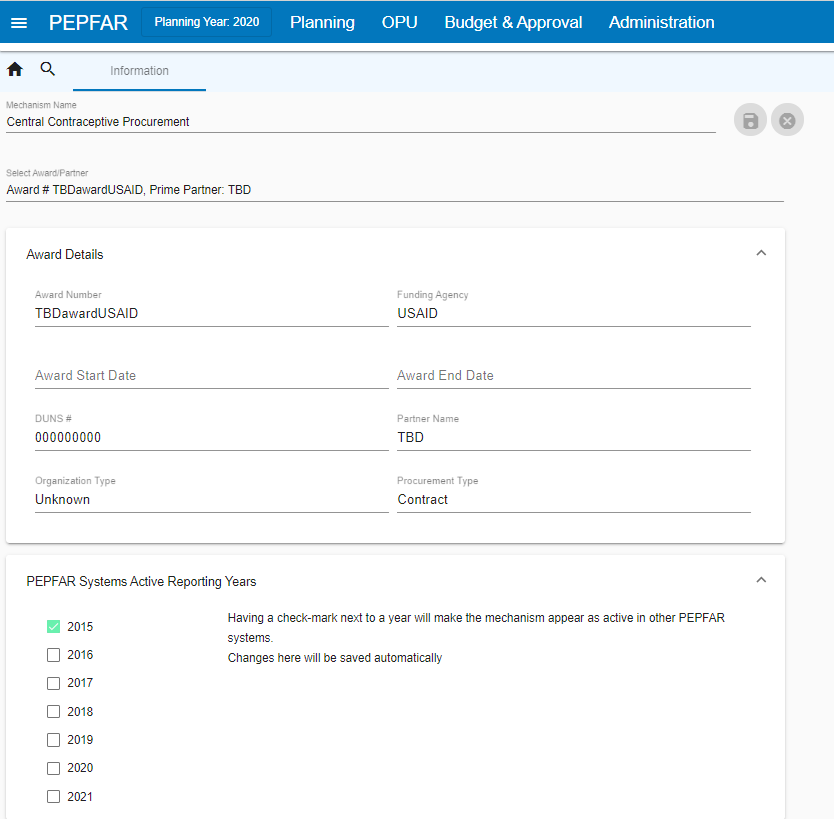
\includegraphics[width=5in]{./images/image15.png}

\end{center}

\hypertarget{note-on-peace-corps-mechanisms}{%
\section{Note on Peace Corps Mechanisms}\label{note-on-peace-corps-mechanisms}}

For the COP21 planning cycle, Peace Corps will transition from reporting
targets under their older mechanisms to reporting all targets under the
Management \& Operations (M\&O) mechanisms. Note that the PSNUxIM tab will
initially populate mechanisms and distributions based on previous year targets,
so users must shift their Peace Corps targets to M\&O mechanisms from their
previous mechanisms by changing the IM reference number at the top of the tab
to the appropriate M\&O IM reference number.

\hypertarget{resolving-rounding-errors}{%
\section{Resolving Rounding Errors}\label{resolving-rounding-errors}}

Due to the combination of multiplication of percentage values against
target values coming from other parts of the Data Pack, and rounding of
all mechanism target values to integers, target values allocated against
mechanisms may roll up with some slight difference from Data Pack
Targets. It may be necessary to iteratively adjust rounding errors and
deduplications throughout the IM allocation process, though in general
it is a good practice to resolve rounding errors as much as possible
before moving on to deduplication. To resolve rounding errors, adjust
percentages gradually, as follows:

\begin{enumerate}
\def\labelenumi{\arabic{enumi})}
\item
  If you had previously unhid the buffer of green Percentage
  Allocation columns (the section between columns K and CG) while
  adding new mechanisms, or the Deduplication columns in columns CH to
  DB, it may be helpful to hide columns in these sections again now to
  more easily see both Percentage Allocations and Target Values at the
  same time on your screen.
\item
  It may also be helpful to review Duplicated Rollup values in columns
  DC to DE in addition to Data Pack Targets in column I so as to
  consider rounding errors distinctly from the impacts of
  deduplication. Note that all when first produced, the PSNUxIM tab
  applies no initial deduplication, so Total Duplicated Rollups and
  Data Pack Targets will match when first received.
\item
  While maintaining overall distribution patterns as intended,
  gradually adjust percentage allocations under affected mechanisms in
  columns K through CG to increase or decrease Duplicated Rollups as
  needed.
\end{enumerate}

Note that while all rounding errors should be resolved if possible, a
small margin of error around some values is permissible, so long as this
does not exceed an absolute value of 2 in either direction of the Data
Pack Target in column I.

\hypertarget{performing-deduplication}{%
\section{Performing Deduplication}\label{performing-deduplication}}

Follow the below steps to perform all Deduplication associated with IM
allocations of targets. Note that due to improvements to the COP21 Data
Pack and close alignment with DATIM, performing deduplications in the
Data Pack resolves the need to perform any deduplication in DATIM.

\begin{enumerate}
\def\labelenumi{\arabic{enumi}.}
\item
  If you had previously unhid the buffer of green Percentage
  Allocation columns (columns K -- CG), it may be helpful to hide
  empty columns in this section again now.
\item
  Review Duplicated Rollups for DSD, TA, and total targets, beginning
  in column DC. These are dynamically summed across all mechanism
  targets allocated in the PSNU x IM tab to the right of these
  columns. To adjust these totals, return to the Percentage Allocation
  section.
\item
  Review TA Deduplication in columns CV to DB, DSD Deduplication in
  columns CO to CU, and Crosswalk Deduplication in columns CH to CN
  (recommended in that order for each row):

  \begin{enumerate}
  \def\labelenumii{\alph{enumii}.}
  \item
    Where only a single mechanism is assigned targets under either
    DSD or TA (for DSD and TA Deduplication), where deduplicated DSD
    and TA totals (see column CH) aggregate to less than or equal to
    Data Pack targets (for Crosswalk Deduplication), or where total
    mechanism targets (column DC) aggregate to less than or equal to
    Data Pack Targets (column I), gray highlighting in these
    sections indicates that deduplication is not necessary or
    permitted.
  \item
    Review allowable ranges for possible deduplicated totals by
    referencing the SUM and MAX rollup columns. As in the DATIM
    Deduplication App, SUM values represent cases with zero
    deduplication, and MAX rollups represent application of the most
    deduplication possible, resulting in values equivalent to the
    largest IM target among either the DSD or TA mechanisms (for DSD
    or TA deduplication), or the larger of either DSD or TA
    deduplicated totals (for crosswalk deduplication).
  \item
    Review Observed Dedupe Resolutions seen in FY21 Target
    allocations. These are provided for reference, and indicate
    which deduplication approach was used in FY21 Target
    deduplication, performed in the DATIM Deduplication App.
  \item
    For cases where Custom deduplication was used in FY21 Targets,
    review the Custom Dedupe Allocation observed in FY21 Targets.
    Percentages here are calculated by dividing the DSD or TA
    deduplication value (for DSD or TA deduplication) or the sum of
    Deduplicated DSD and Deduplicated TA (for crosswalk
    deduplication) by the sum of all mechanisms and deduplication
    values, across both DSD and TA. As such, these values are all
    negative or zero, and can be easily compared against target
    allocation percentages used in columns K -- CG.
  \item
    In columns CZ for TA, CS for DSD, and CL for Crosswalk, manually
    type the deduplication resolution approach to be used to resolve
    deduplication issues, as follows:

    \begin{enumerate}
    \def\labelenumiii{\roman{enumiii}.}
    \item
      ``CUSTOM'' or ``custom'' or ``Custom''
    \item
      ``SUM'' or ``sum'' or ``Sum''
    \item
      ``MAX'' or ``max'' or ``Max''
    \end{enumerate}
  \item
    Where Custom deduplication is selected, also indicate the
    percentage allocation to be assigned to the deduplication value
    in the column to the immediate right. Again, a reminder that
    these values should all be negative or zero, and represent the
    proportion of deduplication values relative to the Data Pack
    Target total in column I. Initially upon indicating Custom
    deduplication, the Data Pack will preset this deduplication
    allocation equal to the value observed in FY21 Targets, if any.
    You may alter and adjust this value as needed, so long as it is
    negative or zero. Also note that it is not enough to only type
    in a percentage deduplication allocation; you must also enter
    ``CUSTOM'', ``SUM'', or ``MAX'', as explained in the previous step.
    Note that instead of entering ``SUM'', it is possible to enter
    ``CUSTOM'' but enter a deduplication percentage allocation of 0\%;
    and instead of entering ``MAX'', it is possible to enter ``CUSTOM''
    but enter a deduplication percentage allocation that results in
    the equivalent of the MAX value shown in columns CI, CP, or CW.
  \end{enumerate}
\item
  Review the Rollup values in column J for any mismatch against Data
  Pack Targets in column I that may necessitate adjustment of
  Deduplication allocations. Note that while it is not a strict
  requirement that percentage allocations across mechanisms and
  deduplication add to 100\%, it is a requirement that integer values
  add to equal the Data Pack Target in column I, ± 2. Red highlights
  in column J indicate values more than 2 (integer, absolute value)
  away from the Data Pack Targets in column I; yellow highlights
  indicate values 1 or 2 (integer, absolute value) away from the Data
  Pack Targets column I.
\end{enumerate}

\elandscape

\newpage

\blandscape

\hypertarget{appendix}{%
\chapter{Appendix}\label{appendix}}

\hypertarget{reference-materials}{%
\section{Reference Materials}\label{reference-materials}}

\begin{itemize}
\item
  COP/ROP 2021 Guidance:
  \url{https://www.state.gov/wp-content/uploads/2020/12/PEPFAR-COP21-Guidance-Final.pdf}
\item
  MER Data Validation Rules User Guide:
  \url{https://datim.zendesk.com/hc/en-us/articles/360055112711-MER-Validation-Guide}

  \begin{itemize}
  \tightlist
  \item
    This Document has been designed to communicate all validation
    rules that the Data Pack, as well as other COP21 documents, will
    go through in the validation and upload process. A description
    of the validation rules, their definitions and user actions to
    correct any flagged errors can be found in this document.
  \end{itemize}
\item
  Monitoring, Evaluation, and Reporting Indicator Reference Guide
  (MER) v2.5:
  \url{https://datim.zendesk.com/hc/en-us/articles/360000084446-MER-Indicator-Reference-Guides}
\item
  MER 2.5 Training Videos:
  \url{https://datim.zendesk.com/hc/en-us/articles/360051593031-MER-2-5-Training-Videos}
\end{itemize}

\elandscape

\end{document}
